\documentclass[twoside]{book}

% Packages required by doxygen
\usepackage{fixltx2e}
\usepackage{calc}
\usepackage{doxygen}
\usepackage[export]{adjustbox} % also loads graphicx
\usepackage{graphicx}
\usepackage[utf8]{inputenc}
\usepackage{makeidx}
\usepackage{multicol}
\usepackage{multirow}
\PassOptionsToPackage{warn}{textcomp}
\usepackage{textcomp}
\usepackage[nointegrals]{wasysym}
\usepackage[table]{xcolor}

% Font selection
\usepackage[T1]{fontenc}
\usepackage[scaled=.90]{helvet}
\usepackage{courier}
\usepackage{amssymb}
\usepackage{sectsty}
\renewcommand{\familydefault}{\sfdefault}
\allsectionsfont{%
  \fontseries{bc}\selectfont%
  \color{darkgray}%
}
\renewcommand{\DoxyLabelFont}{%
  \fontseries{bc}\selectfont%
  \color{darkgray}%
}
\newcommand{\+}{\discretionary{\mbox{\scriptsize$\hookleftarrow$}}{}{}}

% Page & text layout
\usepackage{geometry}
\geometry{%
  a4paper,%
  top=2.5cm,%
  bottom=2.5cm,%
  left=2.5cm,%
  right=2.5cm%
}
\tolerance=750
\hfuzz=15pt
\hbadness=750
\setlength{\emergencystretch}{15pt}
\setlength{\parindent}{0cm}
\setlength{\parskip}{0.2cm}
\makeatletter
\renewcommand{\paragraph}{%
  \@startsection{paragraph}{4}{0ex}{-1.0ex}{1.0ex}{%
    \normalfont\normalsize\bfseries\SS@parafont%
  }%
}
\renewcommand{\subparagraph}{%
  \@startsection{subparagraph}{5}{0ex}{-1.0ex}{1.0ex}{%
    \normalfont\normalsize\bfseries\SS@subparafont%
  }%
}
\makeatother

% Headers & footers
\usepackage{fancyhdr}
\pagestyle{fancyplain}
\fancyhead[LE]{\fancyplain{}{\bfseries\thepage}}
\fancyhead[CE]{\fancyplain{}{}}
\fancyhead[RE]{\fancyplain{}{\bfseries\leftmark}}
\fancyhead[LO]{\fancyplain{}{\bfseries\rightmark}}
\fancyhead[CO]{\fancyplain{}{}}
\fancyhead[RO]{\fancyplain{}{\bfseries\thepage}}
\fancyfoot[LE]{\fancyplain{}{}}
\fancyfoot[CE]{\fancyplain{}{}}
\fancyfoot[RE]{\fancyplain{}{\bfseries\scriptsize Generated on Fri Jul 31 2015 14\+:41\+:25 for My Project by Doxygen }}
\fancyfoot[LO]{\fancyplain{}{\bfseries\scriptsize Generated on Fri Jul 31 2015 14\+:41\+:25 for My Project by Doxygen }}
\fancyfoot[CO]{\fancyplain{}{}}
\fancyfoot[RO]{\fancyplain{}{}}
\renewcommand{\footrulewidth}{0.4pt}
\renewcommand{\chaptermark}[1]{%
  \markboth{#1}{}%
}
\renewcommand{\sectionmark}[1]{%
  \markright{\thesection\ #1}%
}

% Indices & bibliography
\usepackage{natbib}
\usepackage[titles]{tocloft}
\setcounter{tocdepth}{3}
\setcounter{secnumdepth}{5}
\makeindex

% Hyperlinks (required, but should be loaded last)
\usepackage{ifpdf}
\ifpdf
  \usepackage[pdftex,pagebackref=true]{hyperref}
\else
  \usepackage[ps2pdf,pagebackref=true]{hyperref}
\fi
\hypersetup{%
  colorlinks=true,%
  linkcolor=blue,%
  citecolor=blue,%
  unicode%
}

% Custom commands
\newcommand{\clearemptydoublepage}{%
  \newpage{\pagestyle{empty}\cleardoublepage}%
}


%===== C O N T E N T S =====

\begin{document}

% Titlepage & ToC
\hypersetup{pageanchor=false,
             bookmarks=true,
             bookmarksnumbered=true,
             pdfencoding=unicode
            }
\pagenumbering{roman}
\begin{titlepage}
\vspace*{7cm}
\begin{center}%
{\Large My Project }\\
\vspace*{1cm}
{\large Generated by Doxygen 1.8.9.1}\\
\vspace*{0.5cm}
{\small Fri Jul 31 2015 14:41:25}\\
\end{center}
\end{titlepage}
\clearemptydoublepage
\tableofcontents
\clearemptydoublepage
\pagenumbering{arabic}
\hypersetup{pageanchor=true}

%--- Begin generated contents ---
\chapter{Hierarchical Index}
\section{Class Hierarchy}
This inheritance list is sorted roughly, but not completely, alphabetically\+:\begin{DoxyCompactList}
\item \contentsline{section}{Component}{\pageref{class_component}}{}
\begin{DoxyCompactList}
\item \contentsline{section}{C\+Children}{\pageref{class_c_children}}{}
\item \contentsline{section}{C\+Color}{\pageref{class_c_color}}{}
\item \contentsline{section}{C\+Draw}{\pageref{class_c_draw}}{}
\begin{DoxyCompactList}
\item \contentsline{section}{C\+Draw\+Button}{\pageref{class_c_draw_button}}{}
\item \contentsline{section}{C\+Draw\+Circle}{\pageref{class_c_draw_circle}}{}
\item \contentsline{section}{C\+Draw\+Ghost}{\pageref{class_c_draw_ghost}}{}
\item \contentsline{section}{C\+Draw\+Image}{\pageref{class_c_draw_image}}{}
\item \contentsline{section}{C\+Draw\+Label}{\pageref{class_c_draw_label}}{}
\item \contentsline{section}{C\+Draw\+Line}{\pageref{class_c_draw_line}}{}
\item \contentsline{section}{C\+Draw\+Rectangle}{\pageref{class_c_draw_rectangle}}{}
\item \contentsline{section}{C\+Draw\+Text\+Box}{\pageref{class_c_draw_text_box}}{}
\item \contentsline{section}{C\+Draw\+Triangle}{\pageref{class_c_draw_triangle}}{}
\end{DoxyCompactList}
\item \contentsline{section}{C\+Event}{\pageref{class_c_event}}{}
\item \contentsline{section}{C\+Geometry}{\pageref{class_c_geometry}}{}
\item \contentsline{section}{C\+Identifier}{\pageref{class_c_identifier}}{}
\item \contentsline{section}{C\+Label}{\pageref{class_c_label}}{}
\end{DoxyCompactList}
\item \contentsline{section}{Entity}{\pageref{class_entity}}{}
\item \contentsline{section}{Factory}{\pageref{class_factory}}{}
\item \contentsline{section}{S\+Render}{\pageref{class_s_render}}{}
\end{DoxyCompactList}

\chapter{Class Index}
\section{Class List}
Here are the classes, structs, unions and interfaces with brief descriptions\+:\begin{DoxyCompactList}
\item\contentsline{section}{\hyperlink{class_c_children}{C\+Children} \\*Classe héritant de \hyperlink{class_component}{Component} et fait d\textquotesingle{}une map d\textquotesingle{}entitée }{\pageref{class_c_children}}{}
\item\contentsline{section}{\hyperlink{class_c_color}{C\+Color} \\*Classe héritant de \hyperlink{class_component}{Component} et composé des variables R\+G\+B\+A }{\pageref{class_c_color}}{}
\item\contentsline{section}{\hyperlink{class_c_draw}{C\+Draw} \\*Classe héritant de \hyperlink{class_component}{Component} et composé du nécéssaire pour afficher }{\pageref{class_c_draw}}{}
\item\contentsline{section}{\hyperlink{class_c_draw_button}{C\+Draw\+Button} \\*Classe héritant de \hyperlink{class_c_draw}{C\+Draw} et qui contient le cadre et le label }{\pageref{class_c_draw_button}}{}
\item\contentsline{section}{\hyperlink{class_c_draw_circle}{C\+Draw\+Circle} \\*Classe héritant de \hyperlink{class_c_draw}{C\+Draw} et qui contient le sf\+::\+Circle\+Shape }{\pageref{class_c_draw_circle}}{}
\item\contentsline{section}{\hyperlink{class_c_draw_ghost}{C\+Draw\+Ghost} \\*Classe héritant de \hyperlink{class_c_draw}{C\+Draw} et qui affiche les enfants }{\pageref{class_c_draw_ghost}}{}
\item\contentsline{section}{\hyperlink{class_c_draw_image}{C\+Draw\+Image} \\*Classe héritant de \hyperlink{class_c_draw}{C\+Draw} et qui affiche une image }{\pageref{class_c_draw_image}}{}
\item\contentsline{section}{\hyperlink{class_c_draw_label}{C\+Draw\+Label} \\*Classe héritant de \hyperlink{class_c_draw}{C\+Draw} et qui affiche un simple texte }{\pageref{class_c_draw_label}}{}
\item\contentsline{section}{\hyperlink{class_c_draw_line}{C\+Draw\+Line} \\*Classe héritant de \hyperlink{class_c_draw}{C\+Draw} et qui affiche une ligne. Les coordonées x1,y1 et x2,y2 sont utilisées }{\pageref{class_c_draw_line}}{}
\item\contentsline{section}{\hyperlink{class_c_draw_rectangle}{C\+Draw\+Rectangle} \\*Classe héritant de \hyperlink{class_c_draw}{C\+Draw} et qui affiche un rectangle plein }{\pageref{class_c_draw_rectangle}}{}
\item\contentsline{section}{\hyperlink{class_c_draw_text_box}{C\+Draw\+Text\+Box} \\*Classe héritant de \hyperlink{class_c_draw}{C\+Draw} et qui affiche un cadre et un texte }{\pageref{class_c_draw_text_box}}{}
\item\contentsline{section}{\hyperlink{class_c_draw_triangle}{C\+Draw\+Triangle} \\*Classe héritant de \hyperlink{class_c_draw}{C\+Draw} et qui affiche un triangle }{\pageref{class_c_draw_triangle}}{}
\item\contentsline{section}{\hyperlink{class_c_event}{C\+Event} \\*Classe héritant de \hyperlink{class_component}{Component} qui gère les Event }{\pageref{class_c_event}}{}
\item\contentsline{section}{\hyperlink{class_c_geometry}{C\+Geometry} \\*Classe héritant de \hyperlink{class_component}{Component} }{\pageref{class_c_geometry}}{}
\item\contentsline{section}{\hyperlink{class_c_identifier}{C\+Identifier} \\*Classe héritant de \hyperlink{class_component}{Component} stockant l\textquotesingle{}id }{\pageref{class_c_identifier}}{}
\item\contentsline{section}{\hyperlink{class_c_label}{C\+Label} \\*Classe héritant de \hyperlink{class_component}{Component} contient le label en string et le fontsize en int }{\pageref{class_c_label}}{}
\item\contentsline{section}{\hyperlink{class_component}{Component} \\*Parent de tous les components }{\pageref{class_component}}{}
\item\contentsline{section}{\hyperlink{class_entity}{Entity} \\*Classe possédant une map de component et gérant les accès }{\pageref{class_entity}}{}
\item\contentsline{section}{\hyperlink{class_factory}{Factory} \\*Classe qui assemble les components pour préparer les objets demandé }{\pageref{class_factory}}{}
\item\contentsline{section}{\hyperlink{class_s_render}{S\+Render} \\*Classe d\textquotesingle{}encapsulation de la lib }{\pageref{class_s_render}}{}
\end{DoxyCompactList}

\chapter{File Index}
\section{File List}
Here is a list of all documented files with brief descriptions\+:\begin{DoxyCompactList}
\item\contentsline{section}{component/\hyperlink{_c_children_8hh}{C\+Children.\+hh} \\*\hyperlink{class_component}{Component} Container }{\pageref{_c_children_8hh}}{}
\item\contentsline{section}{component/\hyperlink{_c_color_8hh}{C\+Color.\+hh} \\*\hyperlink{class_component}{Component} Color }{\pageref{_c_color_8hh}}{}
\item\contentsline{section}{component/\hyperlink{_c_draw_8hh}{C\+Draw.\+hh} \\*\hyperlink{class_component}{Component} draw général }{\pageref{_c_draw_8hh}}{}
\item\contentsline{section}{component/\hyperlink{_c_draw_button_8hh}{C\+Draw\+Button.\+hh} \\*\hyperlink{class_component}{Component} Draw spécialisé du boutton }{\pageref{_c_draw_button_8hh}}{}
\item\contentsline{section}{component/\hyperlink{_c_draw_circle_8hh}{C\+Draw\+Circle.\+hh} \\*\hyperlink{class_component}{Component} Draw spécialisé du cercle }{\pageref{_c_draw_circle_8hh}}{}
\item\contentsline{section}{component/\hyperlink{_c_draw_ghost_8hh}{C\+Draw\+Ghost.\+hh} \\*\hyperlink{class_component}{Component} Draw qui n\textquotesingle{}affiche pas }{\pageref{_c_draw_ghost_8hh}}{}
\item\contentsline{section}{component/\hyperlink{_c_draw_image_8hh}{C\+Draw\+Image.\+hh} \\*\hyperlink{class_component}{Component} Draw une image }{\pageref{_c_draw_image_8hh}}{}
\item\contentsline{section}{component/\hyperlink{_c_draw_label_8hh}{C\+Draw\+Label.\+hh} \\*\hyperlink{class_component}{Component} Draw qui affiche un label }{\pageref{_c_draw_label_8hh}}{}
\item\contentsline{section}{component/\hyperlink{_c_draw_line_8hh}{C\+Draw\+Line.\+hh} \\*\hyperlink{class_component}{Component} Draw qui affiche une ligne }{\pageref{_c_draw_line_8hh}}{}
\item\contentsline{section}{component/\hyperlink{_c_draw_rectangle_8hh}{C\+Draw\+Rectangle.\+hh} \\*\hyperlink{class_component}{Component} Draw qui affiche un rectangle }{\pageref{_c_draw_rectangle_8hh}}{}
\item\contentsline{section}{component/\hyperlink{_c_draw_text_box_8hh}{C\+Draw\+Text\+Box.\+hh} \\*\hyperlink{class_component}{Component} Draw qui affiche un textarea }{\pageref{_c_draw_text_box_8hh}}{}
\item\contentsline{section}{component/\hyperlink{_c_draw_triangle_8hh}{C\+Draw\+Triangle.\+hh} \\*\hyperlink{class_component}{Component} Draw qui affiche un triangle }{\pageref{_c_draw_triangle_8hh}}{}
\item\contentsline{section}{component/\hyperlink{_c_event_8hh}{C\+Event.\+hh} \\*\hyperlink{class_component}{Component} Event qui réagit aux evenements }{\pageref{_c_event_8hh}}{}
\item\contentsline{section}{component/\hyperlink{_c_geometry_8hh}{C\+Geometry.\+hh} \\*\hyperlink{class_component}{Component} Geometry qui stocke toutes les données nécéssaire pour le draw }{\pageref{_c_geometry_8hh}}{}
\item\contentsline{section}{component/\hyperlink{_c_identifier_8hh}{C\+Identifier.\+hh} \\*\hyperlink{class_component}{Component} I\+D qui identifie de manière unique une entité }{\pageref{_c_identifier_8hh}}{}
\item\contentsline{section}{component/\hyperlink{_c_label_8hh}{C\+Label.\+hh} \\*\hyperlink{class_component}{Component} Label qui contient les informations texte }{\pageref{_c_label_8hh}}{}
\item\contentsline{section}{component/\hyperlink{_component_8hh}{Component.\+hh} \\*\hyperlink{class_component}{Component}, classe parent de tous les component }{\pageref{_component_8hh}}{}
\item\contentsline{section}{entity/\hyperlink{_entity_8hh}{Entity.\+hh} \\*Classe container de component }{\pageref{_entity_8hh}}{}
\item\contentsline{section}{factory/\hyperlink{_factory_8hh}{Factory.\+hh} \\*Usine à entité préfabriquée }{\pageref{_factory_8hh}}{}
\item\contentsline{section}{system/\hyperlink{_s_render_8hh}{S\+Render.\+hh} \\*Classe de gestion de la lib }{\pageref{_s_render_8hh}}{}
\end{DoxyCompactList}

\chapter{Class Documentation}
\hypertarget{class_c_children}{}\section{C\+Children Class Reference}
\label{class_c_children}\index{C\+Children@{C\+Children}}


Classe héritant de \hyperlink{class_component}{Component} et fait d\textquotesingle{}une map d\textquotesingle{}entitée.  




{\ttfamily \#include $<$C\+Children.\+hh$>$}

Inheritance diagram for C\+Children\+:\begin{figure}[H]
\begin{center}
\leavevmode
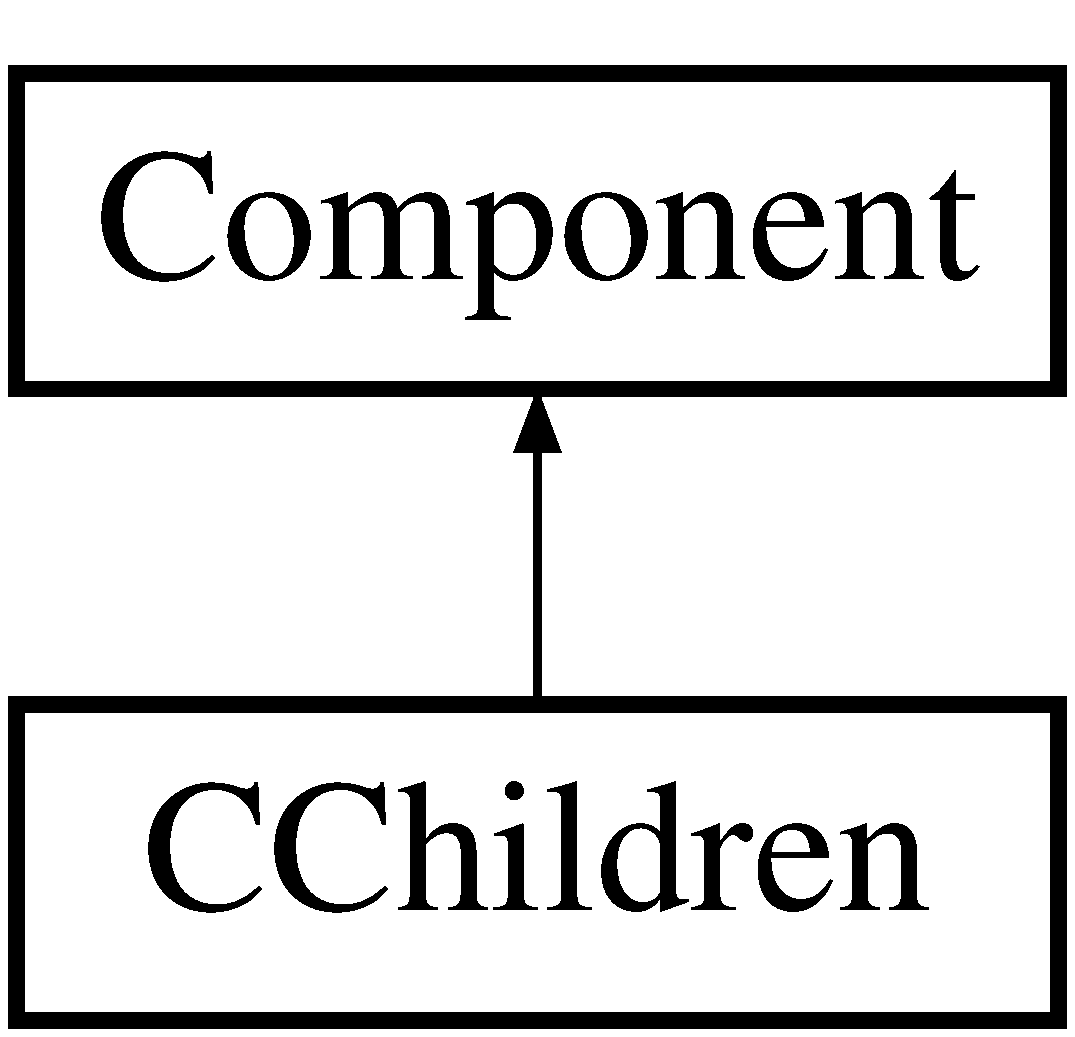
\includegraphics[height=2.000000cm]{class_c_children}
\end{center}
\end{figure}
\subsection*{Public Member Functions}
\begin{DoxyCompactItemize}
\item 
const children\+\_\+map \& \hyperlink{class_c_children_aa02a9a499b3cb60e36d43b049db5dd3a}{get\+All} ()
\begin{DoxyCompactList}\small\item\em Récupérer l\textquotesingle{}ensemble des enfants. \end{DoxyCompactList}\item 
\hyperlink{class_c_children}{C\+Children} $\ast$ \hyperlink{class_c_children_a993c1f483adcba2fee4fbd0e7f13fb33}{push} (\hyperlink{class_entity}{Entity} $\ast$)
\begin{DoxyCompactList}\small\item\em Ajout d\textquotesingle{}une entitée. \end{DoxyCompactList}\item 
\hyperlink{class_c_children}{C\+Children} $\ast$ \hyperlink{class_c_children_a000d123c781df5d6e2000e2799456963}{remove} (int)
\begin{DoxyCompactList}\small\item\em Supression d\textquotesingle{}une entitée. \end{DoxyCompactList}\end{DoxyCompactItemize}
\subsection*{Additional Inherited Members}


\subsection{Detailed Description}
Classe héritant de \hyperlink{class_component}{Component} et fait d\textquotesingle{}une map d\textquotesingle{}entitée. 

\subsection{Member Function Documentation}
\hypertarget{class_c_children_aa02a9a499b3cb60e36d43b049db5dd3a}{}\index{C\+Children@{C\+Children}!get\+All@{get\+All}}
\index{get\+All@{get\+All}!C\+Children@{C\+Children}}
\subsubsection[{get\+All}]{\setlength{\rightskip}{0pt plus 5cm}const children\+\_\+map \& C\+Children\+::get\+All (
\begin{DoxyParamCaption}
{}
\end{DoxyParamCaption}
)}\label{class_c_children_aa02a9a499b3cb60e36d43b049db5dd3a}


Récupérer l\textquotesingle{}ensemble des enfants. 

Methode qui permet de récupérer les enfants de l\textquotesingle{}entitée mère

\begin{DoxyReturn}{Returns}
children\+\_\+map 
\end{DoxyReturn}
\hypertarget{class_c_children_a993c1f483adcba2fee4fbd0e7f13fb33}{}\index{C\+Children@{C\+Children}!push@{push}}
\index{push@{push}!C\+Children@{C\+Children}}
\subsubsection[{push}]{\setlength{\rightskip}{0pt plus 5cm}{\bf C\+Children} $\ast$ C\+Children\+::push (
\begin{DoxyParamCaption}
\item[{{\bf Entity} $\ast$}]{b}
\end{DoxyParamCaption}
)}\label{class_c_children_a993c1f483adcba2fee4fbd0e7f13fb33}


Ajout d\textquotesingle{}une entitée. 

Methode qui permet d\textquotesingle{}ajouter une entitée en tant qu\textquotesingle{}enfant


\begin{DoxyParams}{Parameters}
{\em \hyperlink{class_entity}{Entity}} & $\ast$ \+: l\textquotesingle{}entitée \\
\hline
\end{DoxyParams}
\begin{DoxyReturn}{Returns}
\hyperlink{class_c_children}{C\+Children} $\ast$\+: pour permettre des appels en batterie 
\end{DoxyReturn}
\hypertarget{class_c_children_a000d123c781df5d6e2000e2799456963}{}\index{C\+Children@{C\+Children}!remove@{remove}}
\index{remove@{remove}!C\+Children@{C\+Children}}
\subsubsection[{remove}]{\setlength{\rightskip}{0pt plus 5cm}{\bf C\+Children} $\ast$ C\+Children\+::remove (
\begin{DoxyParamCaption}
\item[{int}]{id}
\end{DoxyParamCaption}
)}\label{class_c_children_a000d123c781df5d6e2000e2799456963}


Supression d\textquotesingle{}une entitée. 

Methode qui permet de supprimer une entitée des enfants


\begin{DoxyParams}{Parameters}
{\em int} & id\+: L\textquotesingle{}id de l\textquotesingle{}entitée a supprimer \\
\hline
\end{DoxyParams}
\begin{DoxyReturn}{Returns}
this pour permettre des appels en batterie 
\end{DoxyReturn}


The documentation for this class was generated from the following files\+:\begin{DoxyCompactItemize}
\item 
component/\hyperlink{_c_children_8hh}{C\+Children.\+hh}\item 
component/C\+Children.\+cpp\end{DoxyCompactItemize}

\hypertarget{class_c_color}{}\section{C\+Color Class Reference}
\label{class_c_color}\index{C\+Color@{C\+Color}}


Classe héritant de \hyperlink{class_component}{Component} et composé des variables R\+G\+B\+A.  




{\ttfamily \#include $<$C\+Color.\+hh$>$}

Inheritance diagram for C\+Color\+:\begin{figure}[H]
\begin{center}
\leavevmode
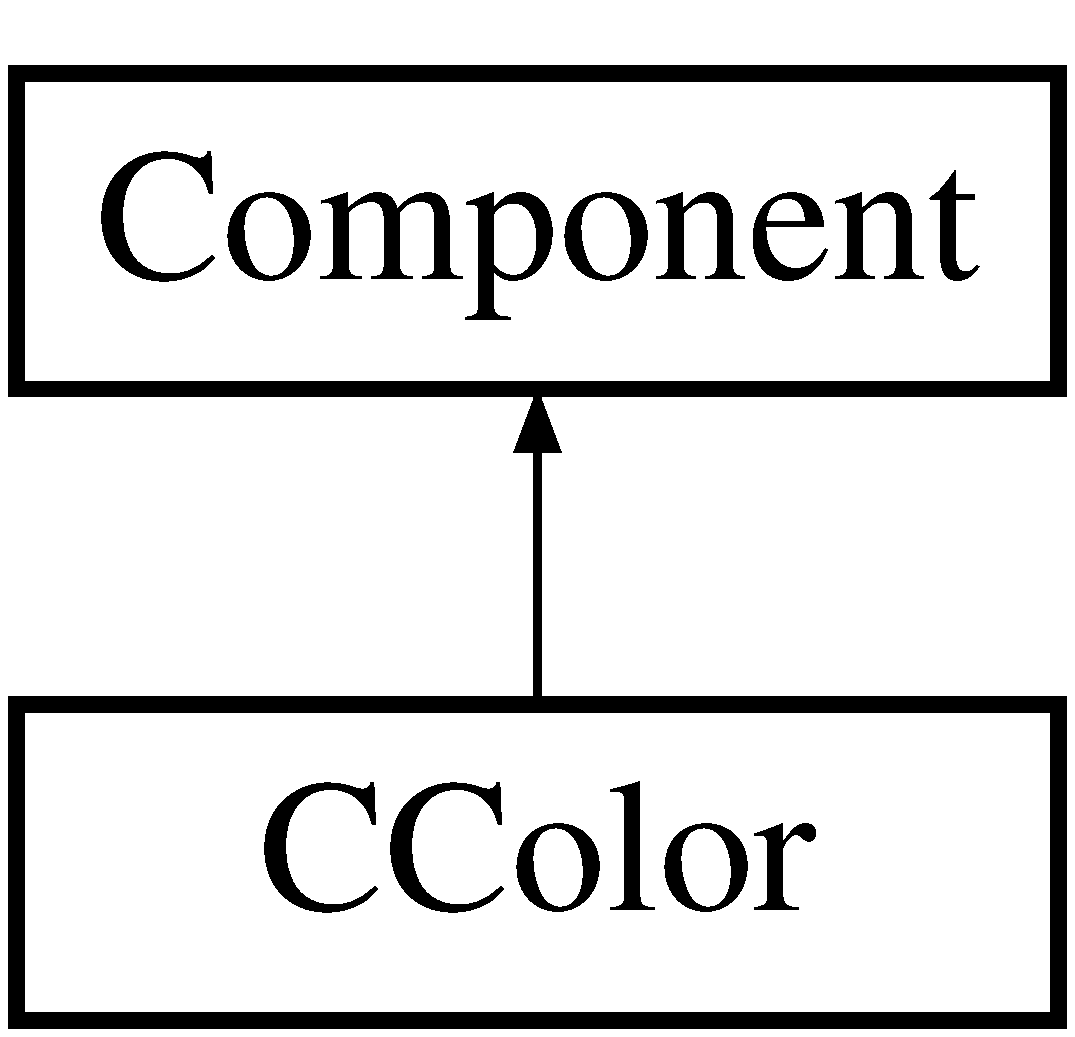
\includegraphics[height=2.000000cm]{class_c_color}
\end{center}
\end{figure}
\subsection*{Public Member Functions}
\begin{DoxyCompactItemize}
\item 
\hyperlink{class_c_color}{C\+Color} $\ast$ \hyperlink{class_c_color_a2e3b83209fb2791bab8a88b833f560e3}{set\+R\+G\+B\+A} (int, int, int, int)
\begin{DoxyCompactList}\small\item\em Setter des 4 variables. \end{DoxyCompactList}\item 
\hyperlink{class_c_color}{C\+Color} $\ast$ \hyperlink{class_c_color_a6efe4461a19fbb302164c38937857c66}{set\+R} (int)
\begin{DoxyCompactList}\small\item\em Setter du canal R\+E\+D. \end{DoxyCompactList}\item 
\hyperlink{class_c_color}{C\+Color} $\ast$ \hyperlink{class_c_color_a942994c75b4d2e416426dc9ec962827b}{set\+G} (int)
\begin{DoxyCompactList}\small\item\em Setter du canal G\+R\+E\+E\+N. \end{DoxyCompactList}\item 
\hyperlink{class_c_color}{C\+Color} $\ast$ \hyperlink{class_c_color_a7a4b8c07c933b84a15a4d47099acc874}{set\+B} (int)
\begin{DoxyCompactList}\small\item\em Setter du canal B\+L\+U\+E. \end{DoxyCompactList}\item 
\hyperlink{class_c_color}{C\+Color} $\ast$ \hyperlink{class_c_color_a2f83c38be2986b5a08ff65466593b8b4}{set\+A} (int)
\begin{DoxyCompactList}\small\item\em Setter du canal A\+L\+P\+H\+A. \end{DoxyCompactList}\item 
void \hyperlink{class_c_color_a8fdd128cecfb6b695bd73bba71e29f5f}{get\+R\+G\+B\+A} (int $\ast$, int $\ast$, int $\ast$, int $\ast$)
\begin{DoxyCompactList}\small\item\em Récupérer l\textquotesingle{}ensemble des couleurs. \end{DoxyCompactList}\item 
int \hyperlink{class_c_color_a774523949afb152bbf2d2a649768088a}{get\+R} ()
\begin{DoxyCompactList}\small\item\em Récupérer la valeur du canal R\+E\+D. \end{DoxyCompactList}\item 
int \hyperlink{class_c_color_a80fbe62e1e7805902d825f8c3f4cf05f}{get\+G} ()
\begin{DoxyCompactList}\small\item\em Récupérer la valeur du canal G\+R\+E\+E\+N. \end{DoxyCompactList}\item 
int \hyperlink{class_c_color_a41f3896ec6410f9082a1b729bffcc763}{get\+B} ()
\begin{DoxyCompactList}\small\item\em Récupérer la valeur du canal B\+L\+U\+E. \end{DoxyCompactList}\item 
int \hyperlink{class_c_color_a553d80922ce6668047020cb5a9189d51}{get\+A} ()
\begin{DoxyCompactList}\small\item\em Récupérer la valeur du canal A\+L\+P\+H\+A. \end{DoxyCompactList}\end{DoxyCompactItemize}
\subsection*{Additional Inherited Members}


\subsection{Detailed Description}
Classe héritant de \hyperlink{class_component}{Component} et composé des variables R\+G\+B\+A. 

\subsection{Member Function Documentation}
\hypertarget{class_c_color_a553d80922ce6668047020cb5a9189d51}{}\index{C\+Color@{C\+Color}!get\+A@{get\+A}}
\index{get\+A@{get\+A}!C\+Color@{C\+Color}}
\subsubsection[{get\+A}]{\setlength{\rightskip}{0pt plus 5cm}int C\+Color\+::get\+A (
\begin{DoxyParamCaption}
{}
\end{DoxyParamCaption}
)}\label{class_c_color_a553d80922ce6668047020cb5a9189d51}


Récupérer la valeur du canal A\+L\+P\+H\+A. 

\begin{DoxyReturn}{Returns}
int alpha 
\end{DoxyReturn}
\hypertarget{class_c_color_a41f3896ec6410f9082a1b729bffcc763}{}\index{C\+Color@{C\+Color}!get\+B@{get\+B}}
\index{get\+B@{get\+B}!C\+Color@{C\+Color}}
\subsubsection[{get\+B}]{\setlength{\rightskip}{0pt plus 5cm}int C\+Color\+::get\+B (
\begin{DoxyParamCaption}
{}
\end{DoxyParamCaption}
)}\label{class_c_color_a41f3896ec6410f9082a1b729bffcc763}


Récupérer la valeur du canal B\+L\+U\+E. 

\begin{DoxyReturn}{Returns}
int blue 
\end{DoxyReturn}
\hypertarget{class_c_color_a80fbe62e1e7805902d825f8c3f4cf05f}{}\index{C\+Color@{C\+Color}!get\+G@{get\+G}}
\index{get\+G@{get\+G}!C\+Color@{C\+Color}}
\subsubsection[{get\+G}]{\setlength{\rightskip}{0pt plus 5cm}int C\+Color\+::get\+G (
\begin{DoxyParamCaption}
{}
\end{DoxyParamCaption}
)}\label{class_c_color_a80fbe62e1e7805902d825f8c3f4cf05f}


Récupérer la valeur du canal G\+R\+E\+E\+N. 

\begin{DoxyReturn}{Returns}
int green 
\end{DoxyReturn}
\hypertarget{class_c_color_a774523949afb152bbf2d2a649768088a}{}\index{C\+Color@{C\+Color}!get\+R@{get\+R}}
\index{get\+R@{get\+R}!C\+Color@{C\+Color}}
\subsubsection[{get\+R}]{\setlength{\rightskip}{0pt plus 5cm}int C\+Color\+::get\+R (
\begin{DoxyParamCaption}
{}
\end{DoxyParamCaption}
)}\label{class_c_color_a774523949afb152bbf2d2a649768088a}


Récupérer la valeur du canal R\+E\+D. 

\begin{DoxyReturn}{Returns}
int red 
\end{DoxyReturn}
\hypertarget{class_c_color_a8fdd128cecfb6b695bd73bba71e29f5f}{}\index{C\+Color@{C\+Color}!get\+R\+G\+B\+A@{get\+R\+G\+B\+A}}
\index{get\+R\+G\+B\+A@{get\+R\+G\+B\+A}!C\+Color@{C\+Color}}
\subsubsection[{get\+R\+G\+B\+A}]{\setlength{\rightskip}{0pt plus 5cm}void C\+Color\+::get\+R\+G\+B\+A (
\begin{DoxyParamCaption}
\item[{int $\ast$}]{\+\_\+r, }
\item[{int $\ast$}]{\+\_\+g, }
\item[{int $\ast$}]{\+\_\+b, }
\item[{int $\ast$}]{\+\_\+a}
\end{DoxyParamCaption}
)}\label{class_c_color_a8fdd128cecfb6b695bd73bba71e29f5f}


Récupérer l\textquotesingle{}ensemble des couleurs. 

Methode qui permet de récupérer les 4 variables en passant des pointeurs sur Int \hypertarget{class_c_color_a2f83c38be2986b5a08ff65466593b8b4}{}\index{C\+Color@{C\+Color}!set\+A@{set\+A}}
\index{set\+A@{set\+A}!C\+Color@{C\+Color}}
\subsubsection[{set\+A}]{\setlength{\rightskip}{0pt plus 5cm}{\bf C\+Color} $\ast$ C\+Color\+::set\+A (
\begin{DoxyParamCaption}
\item[{int}]{\+\_\+a}
\end{DoxyParamCaption}
)}\label{class_c_color_a2f83c38be2986b5a08ff65466593b8b4}


Setter du canal A\+L\+P\+H\+A. 

\begin{DoxyReturn}{Returns}
\hyperlink{class_c_color}{C\+Color} $\ast$this 
\end{DoxyReturn}
\hypertarget{class_c_color_a7a4b8c07c933b84a15a4d47099acc874}{}\index{C\+Color@{C\+Color}!set\+B@{set\+B}}
\index{set\+B@{set\+B}!C\+Color@{C\+Color}}
\subsubsection[{set\+B}]{\setlength{\rightskip}{0pt plus 5cm}{\bf C\+Color} $\ast$ C\+Color\+::set\+B (
\begin{DoxyParamCaption}
\item[{int}]{\+\_\+b}
\end{DoxyParamCaption}
)}\label{class_c_color_a7a4b8c07c933b84a15a4d47099acc874}


Setter du canal B\+L\+U\+E. 

\begin{DoxyReturn}{Returns}
\hyperlink{class_c_color}{C\+Color} $\ast$this 
\end{DoxyReturn}
\hypertarget{class_c_color_a942994c75b4d2e416426dc9ec962827b}{}\index{C\+Color@{C\+Color}!set\+G@{set\+G}}
\index{set\+G@{set\+G}!C\+Color@{C\+Color}}
\subsubsection[{set\+G}]{\setlength{\rightskip}{0pt plus 5cm}{\bf C\+Color} $\ast$ C\+Color\+::set\+G (
\begin{DoxyParamCaption}
\item[{int}]{\+\_\+g}
\end{DoxyParamCaption}
)}\label{class_c_color_a942994c75b4d2e416426dc9ec962827b}


Setter du canal G\+R\+E\+E\+N. 

\begin{DoxyReturn}{Returns}
\hyperlink{class_c_color}{C\+Color} $\ast$this 
\end{DoxyReturn}
\hypertarget{class_c_color_a6efe4461a19fbb302164c38937857c66}{}\index{C\+Color@{C\+Color}!set\+R@{set\+R}}
\index{set\+R@{set\+R}!C\+Color@{C\+Color}}
\subsubsection[{set\+R}]{\setlength{\rightskip}{0pt plus 5cm}{\bf C\+Color} $\ast$ C\+Color\+::set\+R (
\begin{DoxyParamCaption}
\item[{int}]{\+\_\+r}
\end{DoxyParamCaption}
)}\label{class_c_color_a6efe4461a19fbb302164c38937857c66}


Setter du canal R\+E\+D. 

\begin{DoxyReturn}{Returns}
\hyperlink{class_c_color}{C\+Color} $\ast$this 
\end{DoxyReturn}
\hypertarget{class_c_color_a2e3b83209fb2791bab8a88b833f560e3}{}\index{C\+Color@{C\+Color}!set\+R\+G\+B\+A@{set\+R\+G\+B\+A}}
\index{set\+R\+G\+B\+A@{set\+R\+G\+B\+A}!C\+Color@{C\+Color}}
\subsubsection[{set\+R\+G\+B\+A}]{\setlength{\rightskip}{0pt plus 5cm}{\bf C\+Color} $\ast$ C\+Color\+::set\+R\+G\+B\+A (
\begin{DoxyParamCaption}
\item[{int}]{\+\_\+r, }
\item[{int}]{\+\_\+g, }
\item[{int}]{\+\_\+b, }
\item[{int}]{\+\_\+a}
\end{DoxyParamCaption}
)}\label{class_c_color_a2e3b83209fb2791bab8a88b833f560e3}


Setter des 4 variables. 

\begin{DoxyReturn}{Returns}
\hyperlink{class_c_color}{C\+Color} $\ast$this 
\end{DoxyReturn}


The documentation for this class was generated from the following files\+:\begin{DoxyCompactItemize}
\item 
component/\hyperlink{_c_color_8hh}{C\+Color.\+hh}\item 
component/C\+Color.\+cpp\end{DoxyCompactItemize}

\hypertarget{class_c_draw}{}\section{C\+Draw Class Reference}
\label{class_c_draw}\index{C\+Draw@{C\+Draw}}


Classe héritant de \hyperlink{class_component}{Component} et composé du nécéssaire pour afficher.  




{\ttfamily \#include $<$C\+Draw.\+hh$>$}

Inheritance diagram for C\+Draw\+:\begin{figure}[H]
\begin{center}
\leavevmode
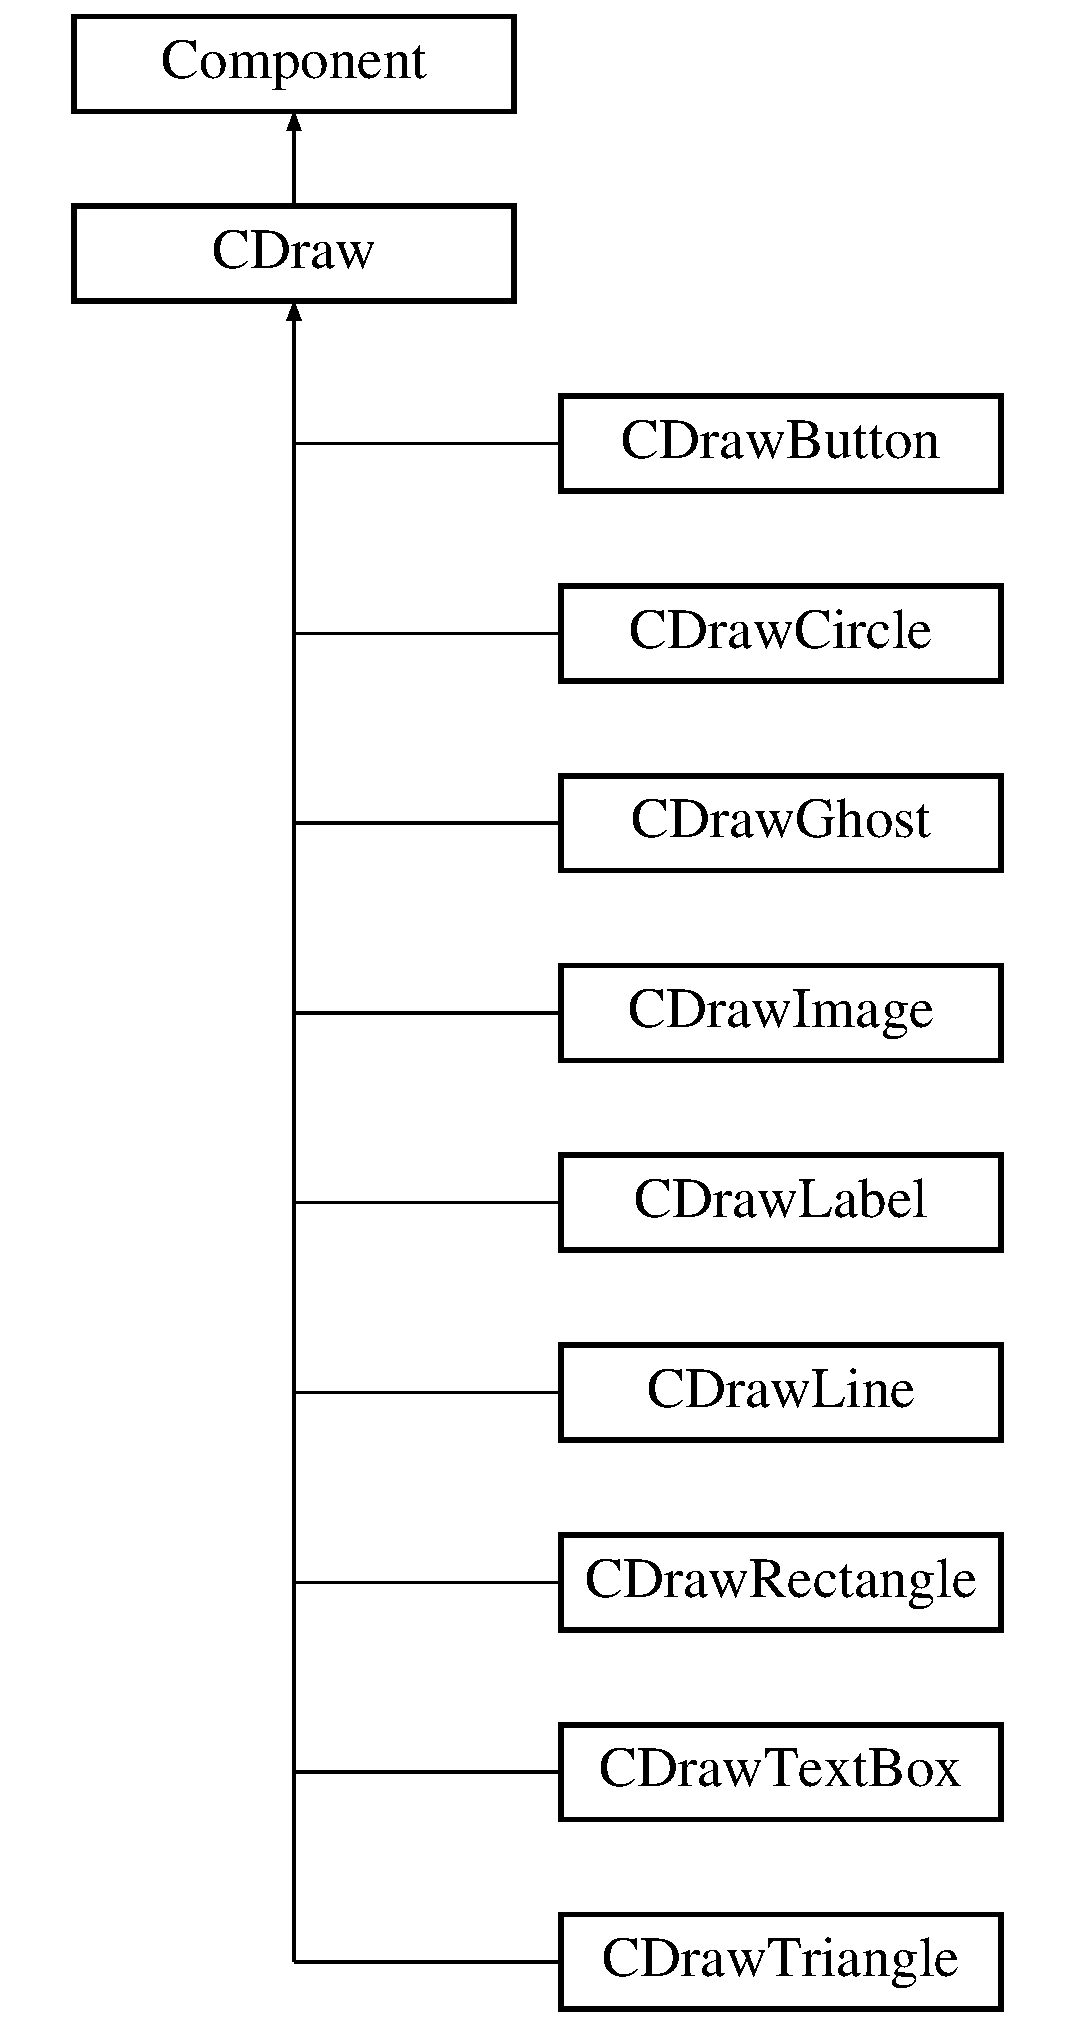
\includegraphics[height=11.000000cm]{class_c_draw}
\end{center}
\end{figure}
\subsection*{Public Member Functions}
\begin{DoxyCompactItemize}
\item 
\hypertarget{class_c_draw_a8750d7c0403a62a0d299d6918233f77c}{}{\bfseries C\+Draw} (\hyperlink{class_s_render}{S\+Render} $\ast$, \hyperlink{class_entity}{Entity} $\ast$)\label{class_c_draw_a8750d7c0403a62a0d299d6918233f77c}

\item 
\hypertarget{class_c_draw_a1f9a4496073715710ae32ed198dae9ab}{}virtual void \hyperlink{class_c_draw_a1f9a4496073715710ae32ed198dae9ab}{draw} ()=0\label{class_c_draw_a1f9a4496073715710ae32ed198dae9ab}

\begin{DoxyCompactList}\small\item\em Fonction draw qui affiche imposée aux enfants. \end{DoxyCompactList}\item 
\hypertarget{class_c_draw_a12c33a831c5a484f4173fbc385e63d72}{}virtual bool \hyperlink{class_c_draw_a12c33a831c5a484f4173fbc385e63d72}{contains} (int, int)=0\label{class_c_draw_a12c33a831c5a484f4173fbc385e63d72}

\begin{DoxyCompactList}\small\item\em Fonction contains qui vérifie si l\textquotesingle{}entité est cliquée. \end{DoxyCompactList}\item 
\hyperlink{class_c_draw}{C\+Draw} $\ast$ \hyperlink{class_c_draw_adc108c63255cf24a18bac9efbd709e8d}{set\+Render} (\hyperlink{class_s_render}{S\+Render} $\ast$)
\begin{DoxyCompactList}\small\item\em En cas de changement de \hyperlink{class_s_render}{S\+Render}. \end{DoxyCompactList}\item 
\hyperlink{class_s_render}{S\+Render} $\ast$ \hyperlink{class_c_draw_a8785e6f252fc6ba0dcf0e1f6faafa06d}{get\+Render} ()
\begin{DoxyCompactList}\small\item\em Getter du render system. \end{DoxyCompactList}\item 
\hypertarget{class_c_draw_a7db62f4578316163367d26a663630ad8}{}void \hyperlink{class_c_draw_a7db62f4578316163367d26a663630ad8}{propagate\+Children} ()\label{class_c_draw_a7db62f4578316163367d26a663630ad8}

\begin{DoxyCompactList}\small\item\em Appel les draws des enfant. \end{DoxyCompactList}\end{DoxyCompactItemize}
\subsection*{Protected Attributes}
\begin{DoxyCompactItemize}
\item 
\hypertarget{class_c_draw_a8a5c5c81cf0975da782ef9684723e964}{}\hyperlink{class_s_render}{S\+Render} $\ast$ {\bfseries o}\label{class_c_draw_a8a5c5c81cf0975da782ef9684723e964}

\item 
\hypertarget{class_c_draw_ab26b641251ce5a8e79e40216348ebc8f}{}\hyperlink{class_entity}{Entity} $\ast$ {\bfseries e}\label{class_c_draw_ab26b641251ce5a8e79e40216348ebc8f}

\item 
\hypertarget{class_c_draw_a29fecb5dbef2702242201c137ed0ee02}{}children\+\_\+map {\bfseries children}\label{class_c_draw_a29fecb5dbef2702242201c137ed0ee02}

\end{DoxyCompactItemize}


\subsection{Detailed Description}
Classe héritant de \hyperlink{class_component}{Component} et composé du nécéssaire pour afficher. 

\hyperlink{class_c_draw}{C\+Draw} stocke un pointeur sur le \hyperlink{class_s_render}{S\+Render} et un pointeur sur l\textquotesingle{}entité actuelle. Le children\+\_\+map contient les enfants de l\textquotesingle{}entité, il est mis à jour en cas de changement. 

\subsection{Member Function Documentation}
\hypertarget{class_c_draw_a8785e6f252fc6ba0dcf0e1f6faafa06d}{}\index{C\+Draw@{C\+Draw}!get\+Render@{get\+Render}}
\index{get\+Render@{get\+Render}!C\+Draw@{C\+Draw}}
\subsubsection[{get\+Render}]{\setlength{\rightskip}{0pt plus 5cm}{\bf S\+Render} $\ast$ C\+Draw\+::get\+Render (
\begin{DoxyParamCaption}
{}
\end{DoxyParamCaption}
)}\label{class_c_draw_a8785e6f252fc6ba0dcf0e1f6faafa06d}


Getter du render system. 

\begin{DoxyReturn}{Returns}
\hyperlink{class_s_render}{S\+Render} $\ast$o 
\end{DoxyReturn}
\hypertarget{class_c_draw_adc108c63255cf24a18bac9efbd709e8d}{}\index{C\+Draw@{C\+Draw}!set\+Render@{set\+Render}}
\index{set\+Render@{set\+Render}!C\+Draw@{C\+Draw}}
\subsubsection[{set\+Render}]{\setlength{\rightskip}{0pt plus 5cm}{\bf C\+Draw} $\ast$ C\+Draw\+::set\+Render (
\begin{DoxyParamCaption}
\item[{{\bf S\+Render} $\ast$}]{\+\_\+o}
\end{DoxyParamCaption}
)}\label{class_c_draw_adc108c63255cf24a18bac9efbd709e8d}


En cas de changement de \hyperlink{class_s_render}{S\+Render}. 

\begin{DoxyReturn}{Returns}
\hyperlink{class_c_draw}{C\+Draw} $\ast$this 
\end{DoxyReturn}


The documentation for this class was generated from the following files\+:\begin{DoxyCompactItemize}
\item 
component/\hyperlink{_c_draw_8hh}{C\+Draw.\+hh}\item 
component/C\+Draw.\+cpp\end{DoxyCompactItemize}

\hypertarget{class_c_draw_button}{}\section{C\+Draw\+Button Class Reference}
\label{class_c_draw_button}\index{C\+Draw\+Button@{C\+Draw\+Button}}


Classe héritant de \hyperlink{class_c_draw}{C\+Draw} et qui contient le cadre et le label.  




{\ttfamily \#include $<$C\+Draw\+Button.\+hh$>$}

Inheritance diagram for C\+Draw\+Button\+:\begin{figure}[H]
\begin{center}
\leavevmode
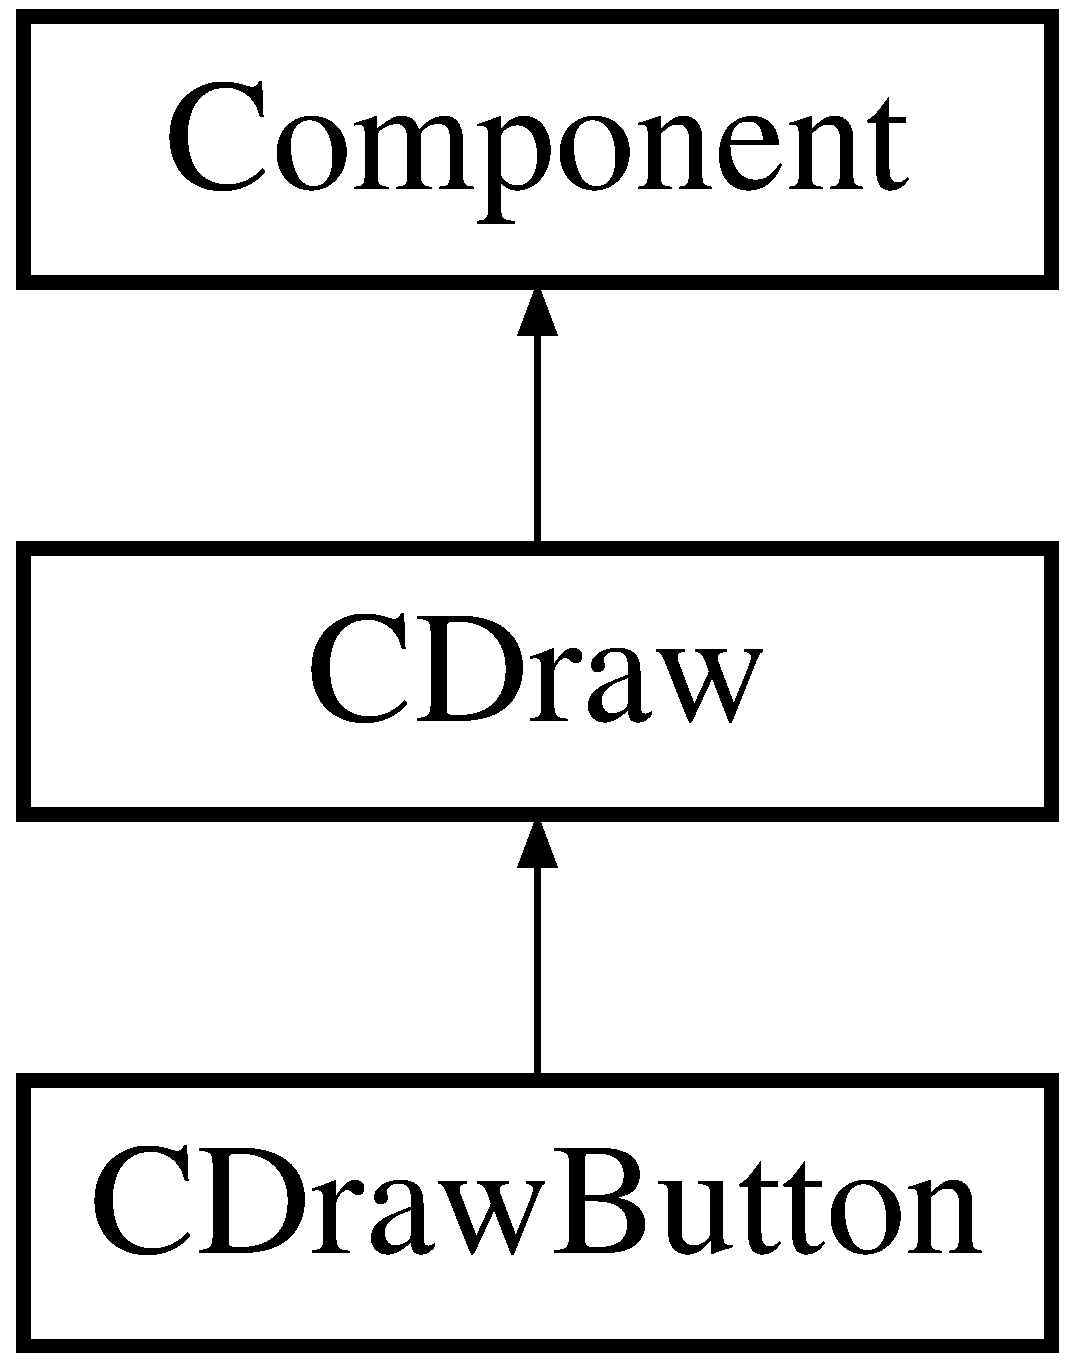
\includegraphics[height=3.000000cm]{class_c_draw_button}
\end{center}
\end{figure}
\subsection*{Public Member Functions}
\begin{DoxyCompactItemize}
\item 
\hypertarget{class_c_draw_button_a02b576eb0c72c556df544876fd6a9677}{}{\bfseries C\+Draw\+Button} (\hyperlink{class_s_render}{S\+Render} $\ast$\+\_\+o, \hyperlink{class_entity}{Entity} $\ast$\+\_\+e)\label{class_c_draw_button_a02b576eb0c72c556df544876fd6a9677}

\item 
\hypertarget{class_c_draw_button_a8499d64ef9d8f8d6478c86352f3be94c}{}void \hyperlink{class_c_draw_button_a8499d64ef9d8f8d6478c86352f3be94c}{init} ()\label{class_c_draw_button_a8499d64ef9d8f8d6478c86352f3be94c}

\begin{DoxyCompactList}\small\item\em Fonction qui va chercher la police du label. \end{DoxyCompactList}\item 
\hypertarget{class_c_draw_button_ab12035c1612138ca17ec3fc3da535247}{}void \hyperlink{class_c_draw_button_ab12035c1612138ca17ec3fc3da535247}{draw} ()\label{class_c_draw_button_ab12035c1612138ca17ec3fc3da535247}

\begin{DoxyCompactList}\small\item\em Affichage du boutton. \end{DoxyCompactList}\item 
bool \hyperlink{class_c_draw_button_a8e8caf8b79a83d0ba38ab0e604a341dc}{contains} (int, int)
\begin{DoxyCompactList}\small\item\em Check si les coordonées sont contenues dans le boutton. \end{DoxyCompactList}\end{DoxyCompactItemize}
\subsection*{Additional Inherited Members}


\subsection{Detailed Description}
Classe héritant de \hyperlink{class_c_draw}{C\+Draw} et qui contient le cadre et le label. 

\subsection{Member Function Documentation}
\hypertarget{class_c_draw_button_a8e8caf8b79a83d0ba38ab0e604a341dc}{}\index{C\+Draw\+Button@{C\+Draw\+Button}!contains@{contains}}
\index{contains@{contains}!C\+Draw\+Button@{C\+Draw\+Button}}
\subsubsection[{contains}]{\setlength{\rightskip}{0pt plus 5cm}bool C\+Draw\+Button\+::contains (
\begin{DoxyParamCaption}
\item[{int}]{\+\_\+x, }
\item[{int}]{\+\_\+y}
\end{DoxyParamCaption}
)\hspace{0.3cm}{\ttfamily [virtual]}}\label{class_c_draw_button_a8e8caf8b79a83d0ba38ab0e604a341dc}


Check si les coordonées sont contenues dans le boutton. 

\begin{DoxyReturn}{Returns}
bool 
\end{DoxyReturn}


Implements \hyperlink{class_c_draw_a12c33a831c5a484f4173fbc385e63d72}{C\+Draw}.



The documentation for this class was generated from the following files\+:\begin{DoxyCompactItemize}
\item 
component/\hyperlink{_c_draw_button_8hh}{C\+Draw\+Button.\+hh}\item 
component/C\+Draw\+Button.\+cpp\end{DoxyCompactItemize}

\hypertarget{class_c_draw_circle}{}\section{C\+Draw\+Circle Class Reference}
\label{class_c_draw_circle}\index{C\+Draw\+Circle@{C\+Draw\+Circle}}


Classe héritant de \hyperlink{class_c_draw}{C\+Draw} et qui contient le sf\+::\+Circle\+Shape.  




{\ttfamily \#include $<$C\+Draw\+Circle.\+hh$>$}

Inheritance diagram for C\+Draw\+Circle\+:\begin{figure}[H]
\begin{center}
\leavevmode
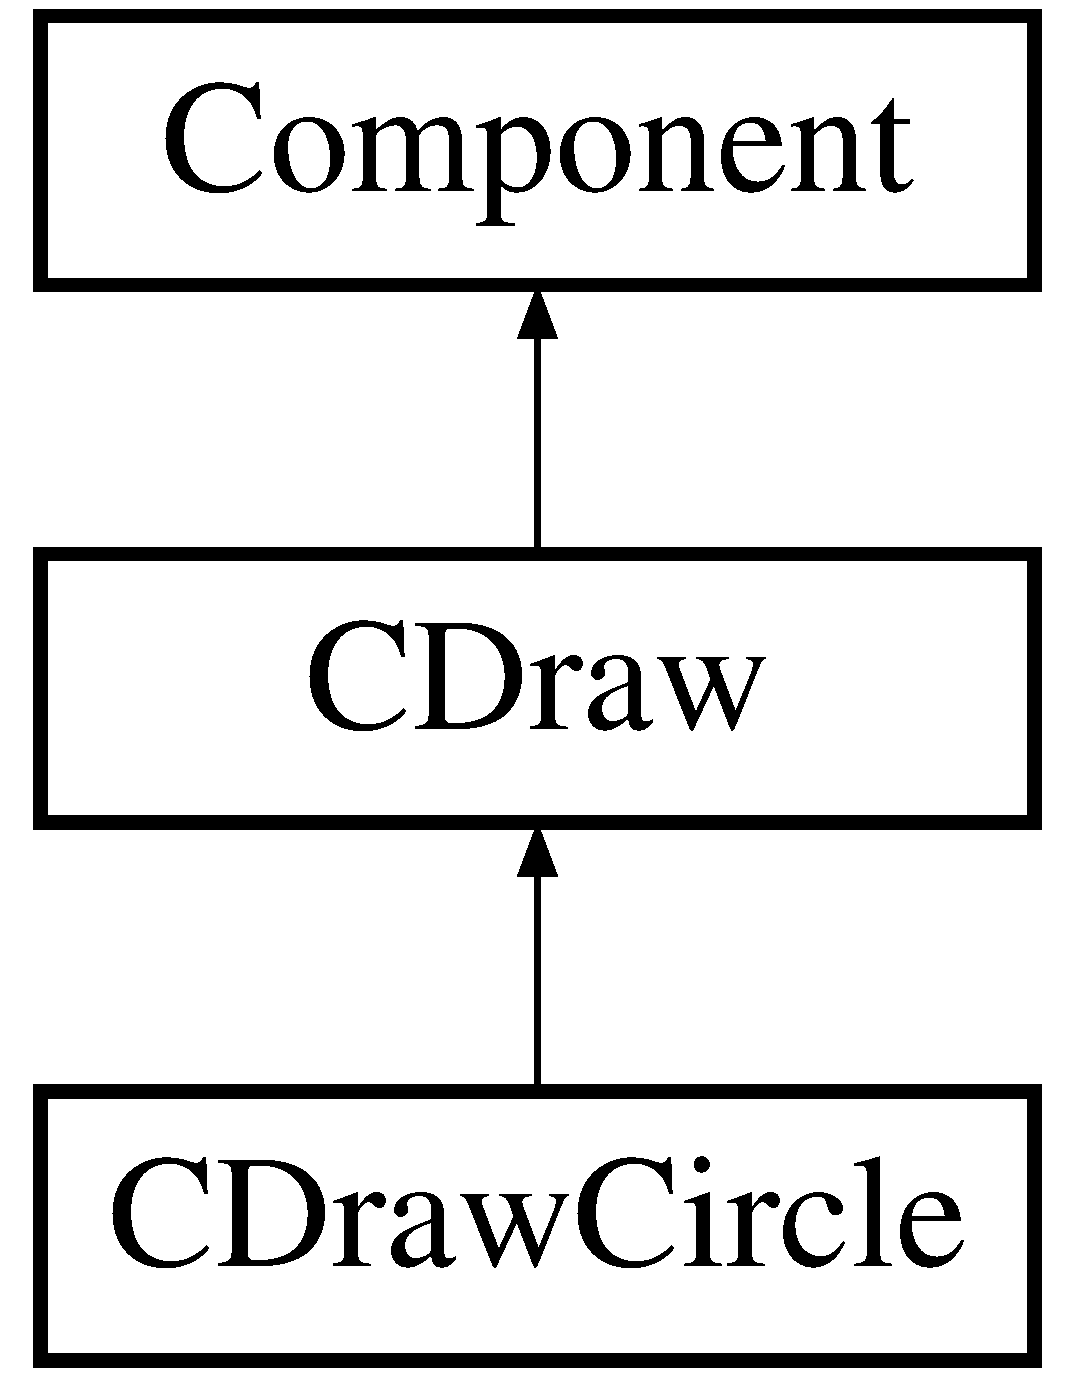
\includegraphics[height=3.000000cm]{class_c_draw_circle}
\end{center}
\end{figure}
\subsection*{Public Member Functions}
\begin{DoxyCompactItemize}
\item 
\hypertarget{class_c_draw_circle_ab04ac44826b605d5712db0057a8319f2}{}{\bfseries C\+Draw\+Circle} (\hyperlink{class_s_render}{S\+Render} $\ast$\+\_\+o, \hyperlink{class_entity}{Entity} $\ast$\+\_\+e)\label{class_c_draw_circle_ab04ac44826b605d5712db0057a8319f2}

\item 
\hypertarget{class_c_draw_circle_ab24d4d6ce1a9baa6354a623641d31df9}{}void \hyperlink{class_c_draw_circle_ab24d4d6ce1a9baa6354a623641d31df9}{draw} ()\label{class_c_draw_circle_ab24d4d6ce1a9baa6354a623641d31df9}

\begin{DoxyCompactList}\small\item\em Affichage du cercle. \end{DoxyCompactList}\item 
bool \hyperlink{class_c_draw_circle_a5e05f05f8b936df0761435e4271b3ba2}{contains} (int, int)
\begin{DoxyCompactList}\small\item\em Check si les coordonées sont contenues dans le cercle. \end{DoxyCompactList}\end{DoxyCompactItemize}
\subsection*{Additional Inherited Members}


\subsection{Detailed Description}
Classe héritant de \hyperlink{class_c_draw}{C\+Draw} et qui contient le sf\+::\+Circle\+Shape. 

\subsection{Member Function Documentation}
\hypertarget{class_c_draw_circle_a5e05f05f8b936df0761435e4271b3ba2}{}\index{C\+Draw\+Circle@{C\+Draw\+Circle}!contains@{contains}}
\index{contains@{contains}!C\+Draw\+Circle@{C\+Draw\+Circle}}
\subsubsection[{contains}]{\setlength{\rightskip}{0pt plus 5cm}bool C\+Draw\+Circle\+::contains (
\begin{DoxyParamCaption}
\item[{int}]{\+\_\+x, }
\item[{int}]{\+\_\+y}
\end{DoxyParamCaption}
)\hspace{0.3cm}{\ttfamily [virtual]}}\label{class_c_draw_circle_a5e05f05f8b936df0761435e4271b3ba2}


Check si les coordonées sont contenues dans le cercle. 

\begin{DoxyReturn}{Returns}
bool 
\end{DoxyReturn}


Implements \hyperlink{class_c_draw_a12c33a831c5a484f4173fbc385e63d72}{C\+Draw}.



The documentation for this class was generated from the following files\+:\begin{DoxyCompactItemize}
\item 
component/\hyperlink{_c_draw_circle_8hh}{C\+Draw\+Circle.\+hh}\item 
component/C\+Draw\+Circle.\+cpp\end{DoxyCompactItemize}

\hypertarget{class_c_draw_ghost}{}\section{C\+Draw\+Ghost Class Reference}
\label{class_c_draw_ghost}\index{C\+Draw\+Ghost@{C\+Draw\+Ghost}}


Classe héritant de \hyperlink{class_c_draw}{C\+Draw} et qui affiche les enfants.  




{\ttfamily \#include $<$C\+Draw\+Ghost.\+hh$>$}

Inheritance diagram for C\+Draw\+Ghost\+:\begin{figure}[H]
\begin{center}
\leavevmode
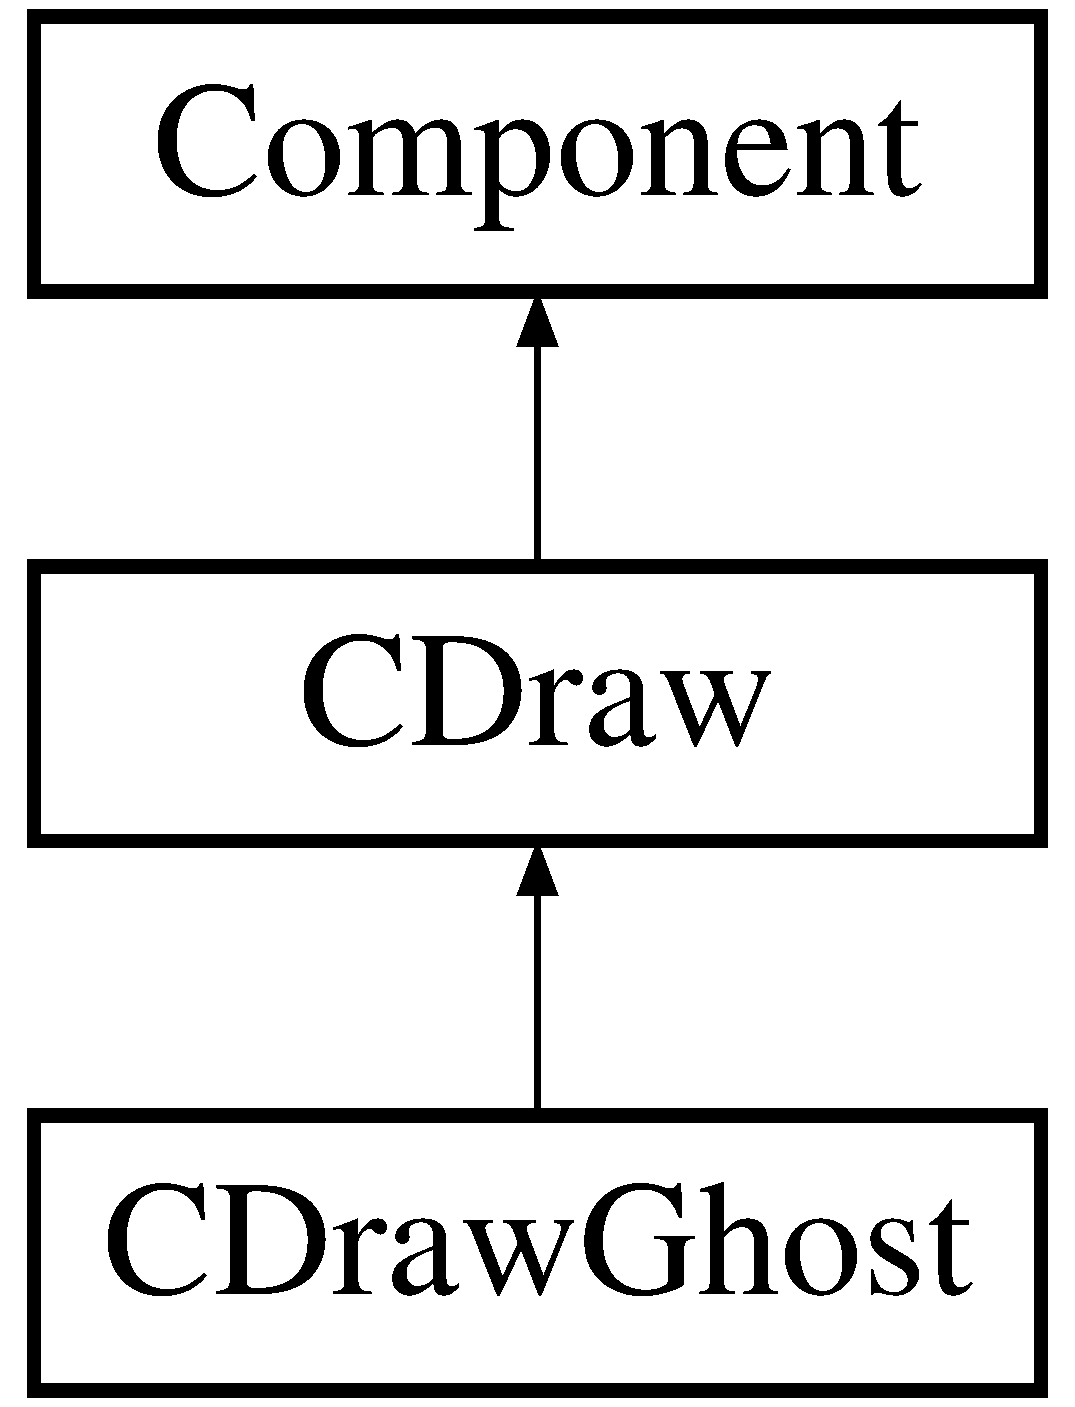
\includegraphics[height=3.000000cm]{class_c_draw_ghost}
\end{center}
\end{figure}
\subsection*{Public Member Functions}
\begin{DoxyCompactItemize}
\item 
\hypertarget{class_c_draw_ghost_a173685c29ad642d905a2b8ffccf03bc6}{}{\bfseries C\+Draw\+Ghost} (\hyperlink{class_entity}{Entity} $\ast$\+\_\+e)\label{class_c_draw_ghost_a173685c29ad642d905a2b8ffccf03bc6}

\item 
bool \hyperlink{class_c_draw_ghost_ae1fbbc9c042292112706fa399e249b35}{contains} (int, int)
\begin{DoxyCompactList}\small\item\em Check si les coordonées sont contenues dans le contenaire. \end{DoxyCompactList}\item 
\hypertarget{class_c_draw_ghost_a4d50d57e38f8eba07c9ba48540e7838c}{}void \hyperlink{class_c_draw_ghost_a4d50d57e38f8eba07c9ba48540e7838c}{draw} ()\label{class_c_draw_ghost_a4d50d57e38f8eba07c9ba48540e7838c}

\begin{DoxyCompactList}\small\item\em N\textquotesingle{}affiche rien. \end{DoxyCompactList}\end{DoxyCompactItemize}
\subsection*{Additional Inherited Members}


\subsection{Detailed Description}
Classe héritant de \hyperlink{class_c_draw}{C\+Draw} et qui affiche les enfants. 

\subsection{Member Function Documentation}
\hypertarget{class_c_draw_ghost_ae1fbbc9c042292112706fa399e249b35}{}\index{C\+Draw\+Ghost@{C\+Draw\+Ghost}!contains@{contains}}
\index{contains@{contains}!C\+Draw\+Ghost@{C\+Draw\+Ghost}}
\subsubsection[{contains}]{\setlength{\rightskip}{0pt plus 5cm}bool C\+Draw\+Ghost\+::contains (
\begin{DoxyParamCaption}
\item[{int}]{x, }
\item[{int}]{y}
\end{DoxyParamCaption}
)\hspace{0.3cm}{\ttfamily [virtual]}}\label{class_c_draw_ghost_ae1fbbc9c042292112706fa399e249b35}


Check si les coordonées sont contenues dans le contenaire. 

\begin{DoxyReturn}{Returns}
bool 
\end{DoxyReturn}


Implements \hyperlink{class_c_draw_a12c33a831c5a484f4173fbc385e63d72}{C\+Draw}.



The documentation for this class was generated from the following files\+:\begin{DoxyCompactItemize}
\item 
component/\hyperlink{_c_draw_ghost_8hh}{C\+Draw\+Ghost.\+hh}\item 
component/C\+Draw\+Ghost.\+cpp\end{DoxyCompactItemize}

\hypertarget{class_c_draw_image}{}\section{C\+Draw\+Image Class Reference}
\label{class_c_draw_image}\index{C\+Draw\+Image@{C\+Draw\+Image}}


Classe héritant de \hyperlink{class_c_draw}{C\+Draw} et qui affiche une image.  




{\ttfamily \#include $<$C\+Draw\+Image.\+hh$>$}

Inheritance diagram for C\+Draw\+Image\+:\begin{figure}[H]
\begin{center}
\leavevmode
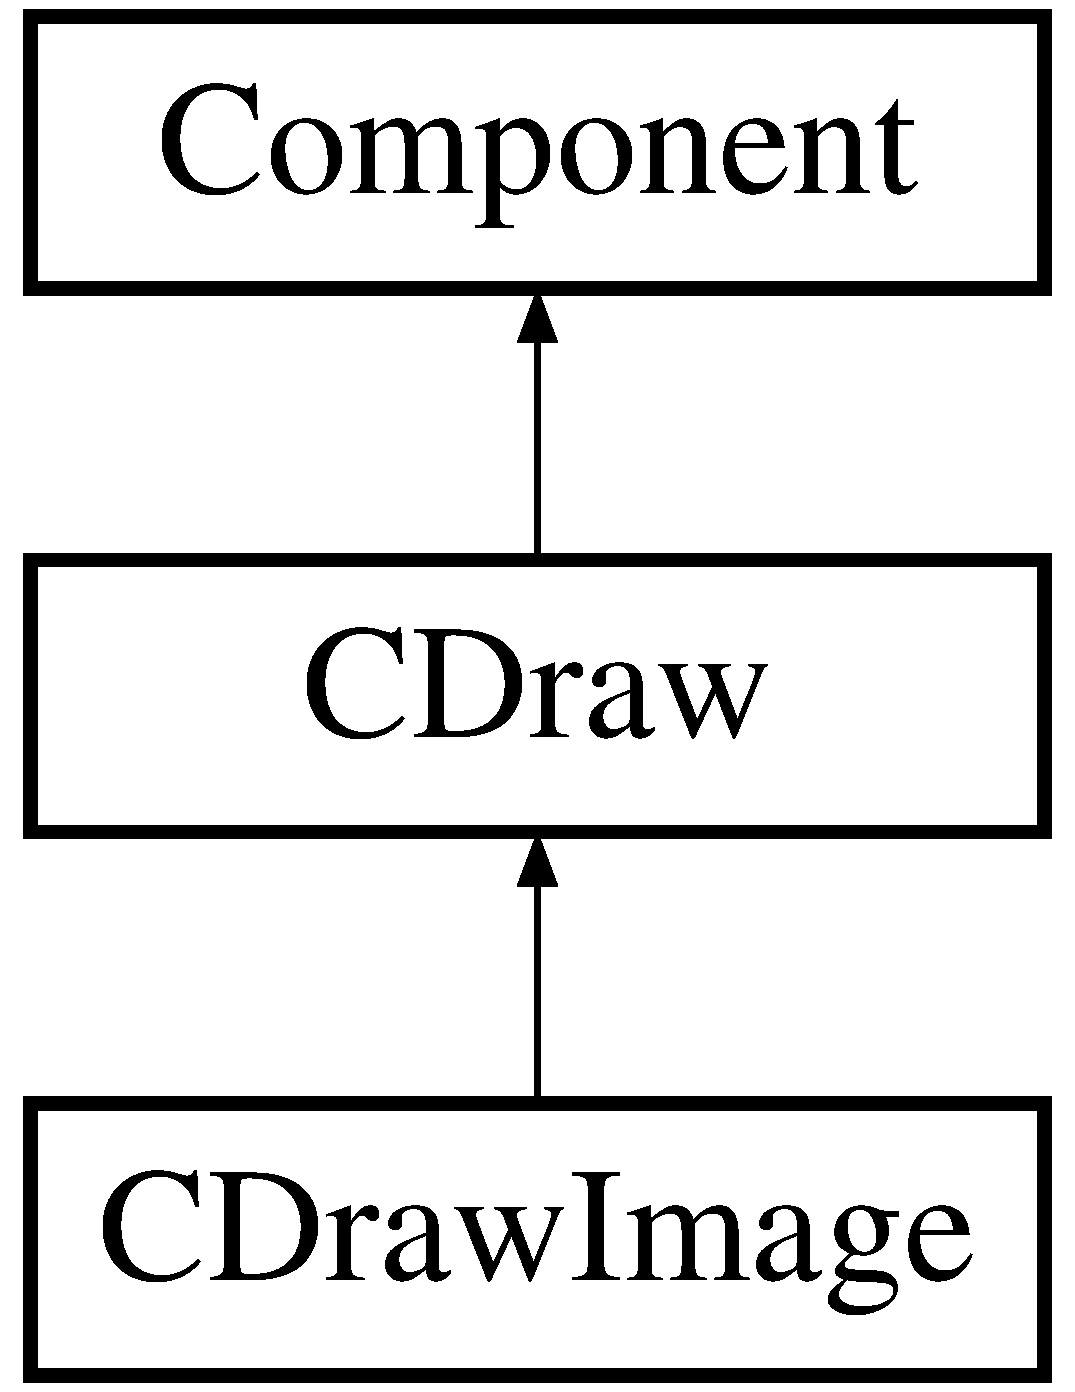
\includegraphics[height=3.000000cm]{class_c_draw_image}
\end{center}
\end{figure}
\subsection*{Public Member Functions}
\begin{DoxyCompactItemize}
\item 
\hypertarget{class_c_draw_image_a62863d288ca481e2d76c90a6b9a27b6a}{}{\bfseries C\+Draw\+Image} (\hyperlink{class_s_render}{S\+Render} $\ast$\+\_\+o, \hyperlink{class_entity}{Entity} $\ast$\+\_\+e)\label{class_c_draw_image_a62863d288ca481e2d76c90a6b9a27b6a}

\item 
\hypertarget{class_c_draw_image_a67e30b0863a13b06436318b3733a0e18}{}void \hyperlink{class_c_draw_image_a67e30b0863a13b06436318b3733a0e18}{draw} ()\label{class_c_draw_image_a67e30b0863a13b06436318b3733a0e18}

\begin{DoxyCompactList}\small\item\em Affiche l\textquotesingle{}image. \end{DoxyCompactList}\item 
bool \hyperlink{class_c_draw_image_a69e0ccf81bdf430ec0f3e77a0ce81e28}{contains} (int, int)
\begin{DoxyCompactList}\small\item\em Check si les coordonées sont contenues dans l\textquotesingle{}image. \end{DoxyCompactList}\end{DoxyCompactItemize}
\subsection*{Additional Inherited Members}


\subsection{Detailed Description}
Classe héritant de \hyperlink{class_c_draw}{C\+Draw} et qui affiche une image. 

La texture est load en cas de changement et le sprite aussi. 

\subsection{Member Function Documentation}
\hypertarget{class_c_draw_image_a69e0ccf81bdf430ec0f3e77a0ce81e28}{}\index{C\+Draw\+Image@{C\+Draw\+Image}!contains@{contains}}
\index{contains@{contains}!C\+Draw\+Image@{C\+Draw\+Image}}
\subsubsection[{contains}]{\setlength{\rightskip}{0pt plus 5cm}bool C\+Draw\+Image\+::contains (
\begin{DoxyParamCaption}
\item[{int}]{\+\_\+x, }
\item[{int}]{\+\_\+y}
\end{DoxyParamCaption}
)\hspace{0.3cm}{\ttfamily [virtual]}}\label{class_c_draw_image_a69e0ccf81bdf430ec0f3e77a0ce81e28}


Check si les coordonées sont contenues dans l\textquotesingle{}image. 

\begin{DoxyReturn}{Returns}
bool 
\end{DoxyReturn}


Implements \hyperlink{class_c_draw_a12c33a831c5a484f4173fbc385e63d72}{C\+Draw}.



The documentation for this class was generated from the following files\+:\begin{DoxyCompactItemize}
\item 
component/\hyperlink{_c_draw_image_8hh}{C\+Draw\+Image.\+hh}\item 
component/C\+Draw\+Image.\+cpp\end{DoxyCompactItemize}

\hypertarget{class_c_draw_label}{}\section{C\+Draw\+Label Class Reference}
\label{class_c_draw_label}\index{C\+Draw\+Label@{C\+Draw\+Label}}


Classe héritant de \hyperlink{class_c_draw}{C\+Draw} et qui affiche un simple texte.  




{\ttfamily \#include $<$C\+Draw\+Label.\+hh$>$}

Inheritance diagram for C\+Draw\+Label\+:\begin{figure}[H]
\begin{center}
\leavevmode
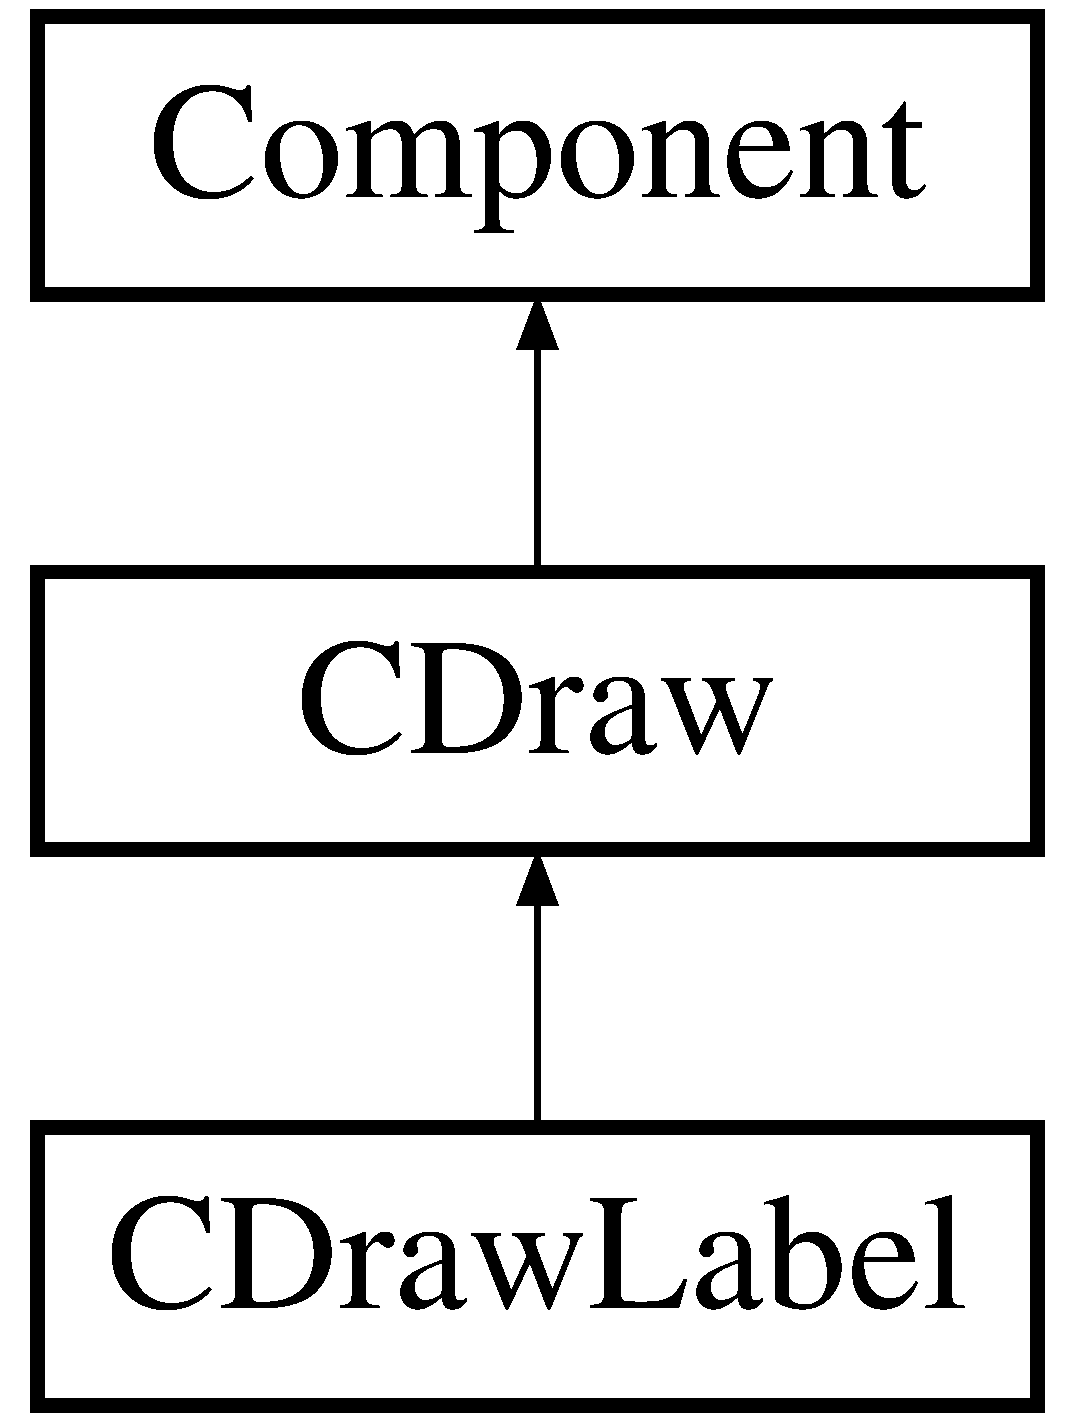
\includegraphics[height=3.000000cm]{class_c_draw_label}
\end{center}
\end{figure}
\subsection*{Public Member Functions}
\begin{DoxyCompactItemize}
\item 
\hypertarget{class_c_draw_label_afd673dace026dfaba16a3ea64f36f026}{}{\bfseries C\+Draw\+Label} (\hyperlink{class_s_render}{S\+Render} $\ast$\+\_\+o, \hyperlink{class_entity}{Entity} $\ast$\+\_\+e)\label{class_c_draw_label_afd673dace026dfaba16a3ea64f36f026}

\item 
\hypertarget{class_c_draw_label_a154fa3e4e641a8bc67866a8d2c2bde51}{}void {\bfseries init} ()\label{class_c_draw_label_a154fa3e4e641a8bc67866a8d2c2bde51}

\item 
\hypertarget{class_c_draw_label_a458ba3fd65336695e34b344ffa787341}{}void \hyperlink{class_c_draw_label_a458ba3fd65336695e34b344ffa787341}{draw} ()\label{class_c_draw_label_a458ba3fd65336695e34b344ffa787341}

\begin{DoxyCompactList}\small\item\em Affiche label. \end{DoxyCompactList}\item 
bool \hyperlink{class_c_draw_label_ac4c633d7443a01fd21d2deef2a055133}{contains} (int, int)
\begin{DoxyCompactList}\small\item\em Check si les coordonées sont contenues dans le rectangle du label. \end{DoxyCompactList}\end{DoxyCompactItemize}
\subsection*{Additional Inherited Members}


\subsection{Detailed Description}
Classe héritant de \hyperlink{class_c_draw}{C\+Draw} et qui affiche un simple texte. 

\subsection{Member Function Documentation}
\hypertarget{class_c_draw_label_ac4c633d7443a01fd21d2deef2a055133}{}\index{C\+Draw\+Label@{C\+Draw\+Label}!contains@{contains}}
\index{contains@{contains}!C\+Draw\+Label@{C\+Draw\+Label}}
\subsubsection[{contains}]{\setlength{\rightskip}{0pt plus 5cm}bool C\+Draw\+Label\+::contains (
\begin{DoxyParamCaption}
\item[{int}]{\+\_\+x, }
\item[{int}]{\+\_\+y}
\end{DoxyParamCaption}
)\hspace{0.3cm}{\ttfamily [virtual]}}\label{class_c_draw_label_ac4c633d7443a01fd21d2deef2a055133}


Check si les coordonées sont contenues dans le rectangle du label. 

\begin{DoxyReturn}{Returns}
bool 
\end{DoxyReturn}


Implements \hyperlink{class_c_draw_a12c33a831c5a484f4173fbc385e63d72}{C\+Draw}.



The documentation for this class was generated from the following files\+:\begin{DoxyCompactItemize}
\item 
component/\hyperlink{_c_draw_label_8hh}{C\+Draw\+Label.\+hh}\item 
component/C\+Draw\+Label.\+cpp\end{DoxyCompactItemize}

\hypertarget{class_c_draw_line}{}\section{C\+Draw\+Line Class Reference}
\label{class_c_draw_line}\index{C\+Draw\+Line@{C\+Draw\+Line}}


Classe héritant de \hyperlink{class_c_draw}{C\+Draw} et qui affiche une ligne. Les coordonées x1,y1 et x2,y2 sont utilisées.  




{\ttfamily \#include $<$C\+Draw\+Line.\+hh$>$}

Inheritance diagram for C\+Draw\+Line\+:\begin{figure}[H]
\begin{center}
\leavevmode
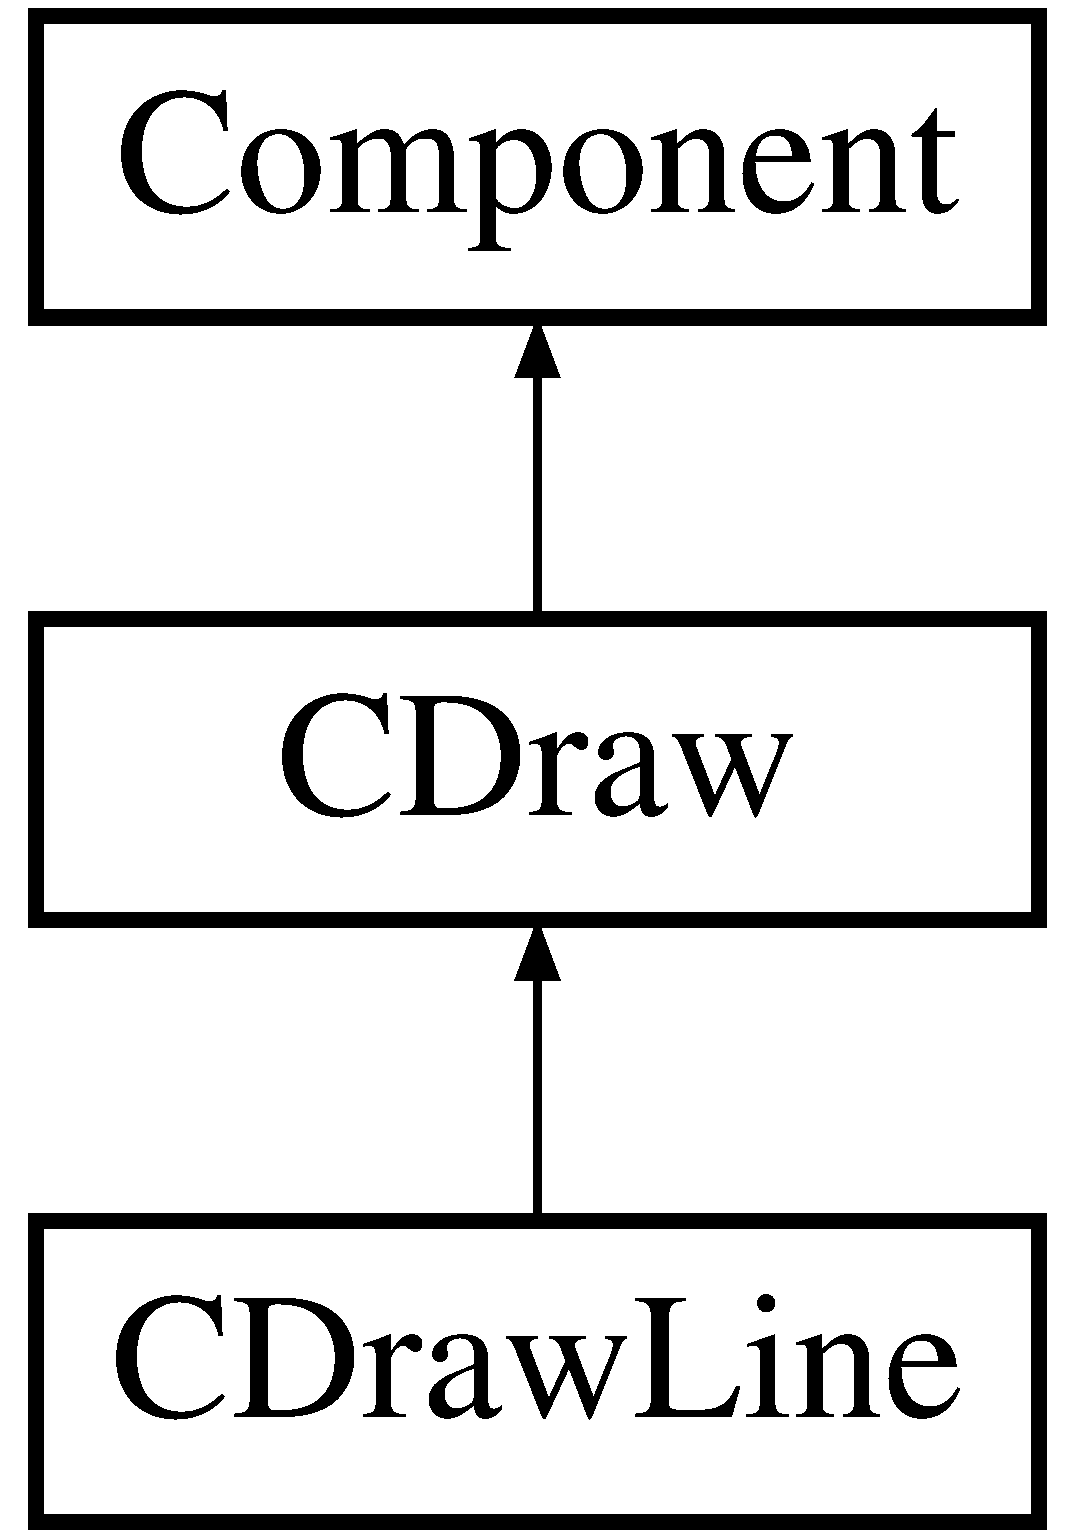
\includegraphics[height=3.000000cm]{class_c_draw_line}
\end{center}
\end{figure}
\subsection*{Public Member Functions}
\begin{DoxyCompactItemize}
\item 
\hypertarget{class_c_draw_line_a8fe36db8c556f007a8a4da97a953c24e}{}{\bfseries C\+Draw\+Line} (\hyperlink{class_s_render}{S\+Render} $\ast$\+\_\+o, \hyperlink{class_entity}{Entity} $\ast$\+\_\+e)\label{class_c_draw_line_a8fe36db8c556f007a8a4da97a953c24e}

\item 
\hypertarget{class_c_draw_line_aaab793b66c3afa04cef25375ab886848}{}void \hyperlink{class_c_draw_line_aaab793b66c3afa04cef25375ab886848}{draw} ()\label{class_c_draw_line_aaab793b66c3afa04cef25375ab886848}

\begin{DoxyCompactList}\small\item\em Affiche la ligne. \end{DoxyCompactList}\item 
bool \hyperlink{class_c_draw_line_a23c866473f91bc6aace37d1bc4250ba9}{contains} (int, int)
\begin{DoxyCompactList}\small\item\em Check si les coordonées sont contenues dans la ligne. \end{DoxyCompactList}\end{DoxyCompactItemize}
\subsection*{Additional Inherited Members}


\subsection{Detailed Description}
Classe héritant de \hyperlink{class_c_draw}{C\+Draw} et qui affiche une ligne. Les coordonées x1,y1 et x2,y2 sont utilisées. 

\subsection{Member Function Documentation}
\hypertarget{class_c_draw_line_a23c866473f91bc6aace37d1bc4250ba9}{}\index{C\+Draw\+Line@{C\+Draw\+Line}!contains@{contains}}
\index{contains@{contains}!C\+Draw\+Line@{C\+Draw\+Line}}
\subsubsection[{contains}]{\setlength{\rightskip}{0pt plus 5cm}bool C\+Draw\+Line\+::contains (
\begin{DoxyParamCaption}
\item[{int}]{x, }
\item[{int}]{y}
\end{DoxyParamCaption}
)\hspace{0.3cm}{\ttfamily [virtual]}}\label{class_c_draw_line_a23c866473f91bc6aace37d1bc4250ba9}


Check si les coordonées sont contenues dans la ligne. 

\begin{DoxyReturn}{Returns}
bool 
\end{DoxyReturn}


Implements \hyperlink{class_c_draw_a12c33a831c5a484f4173fbc385e63d72}{C\+Draw}.



The documentation for this class was generated from the following files\+:\begin{DoxyCompactItemize}
\item 
component/\hyperlink{_c_draw_line_8hh}{C\+Draw\+Line.\+hh}\item 
component/C\+Draw\+Line.\+cpp\end{DoxyCompactItemize}

\hypertarget{class_c_draw_rectangle}{}\section{C\+Draw\+Rectangle Class Reference}
\label{class_c_draw_rectangle}\index{C\+Draw\+Rectangle@{C\+Draw\+Rectangle}}


Classe héritant de \hyperlink{class_c_draw}{C\+Draw} et qui affiche un rectangle plein.  




{\ttfamily \#include $<$C\+Draw\+Rectangle.\+hh$>$}

Inheritance diagram for C\+Draw\+Rectangle\+:\begin{figure}[H]
\begin{center}
\leavevmode
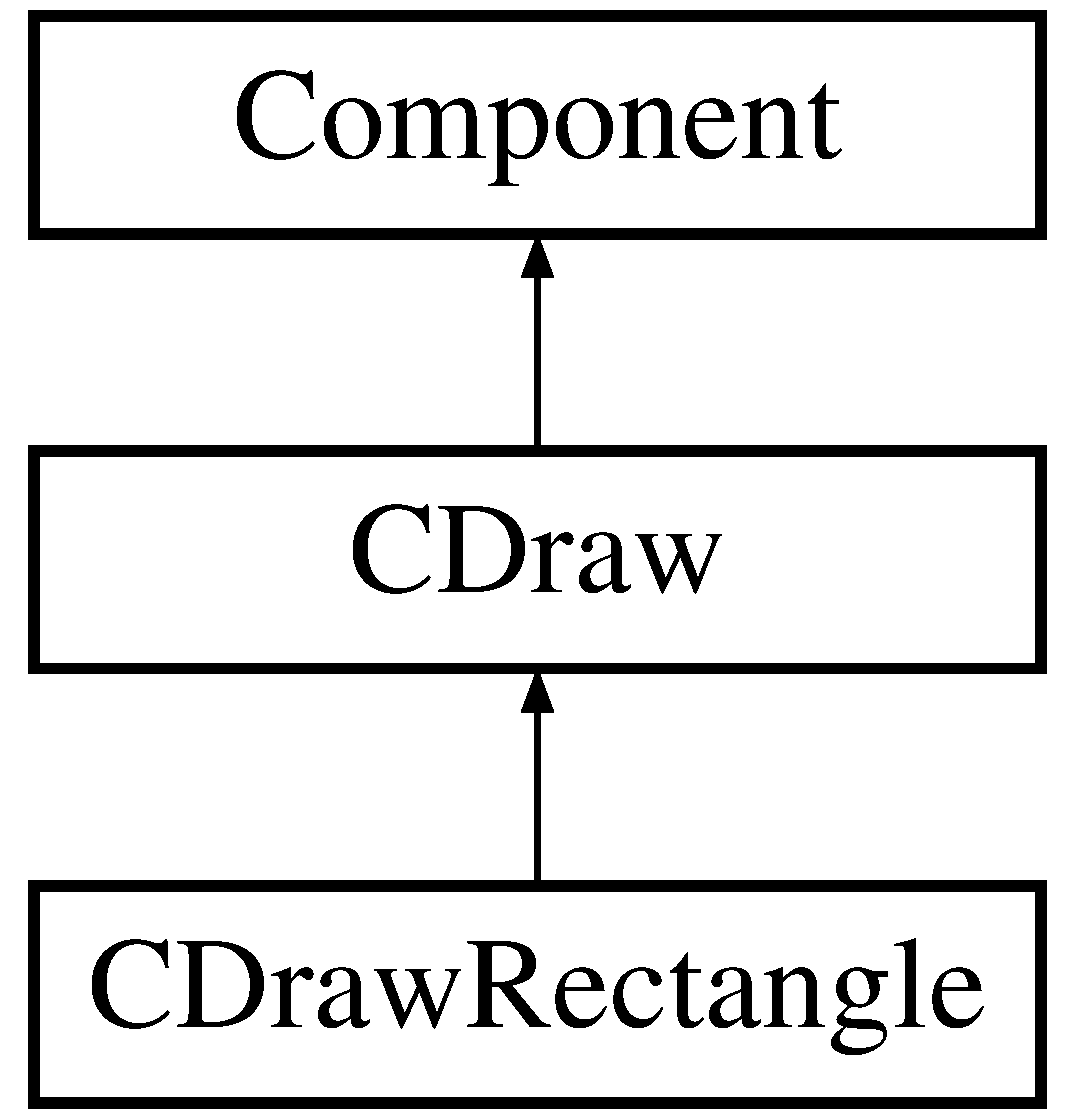
\includegraphics[height=3.000000cm]{class_c_draw_rectangle}
\end{center}
\end{figure}
\subsection*{Public Member Functions}
\begin{DoxyCompactItemize}
\item 
\hypertarget{class_c_draw_rectangle_a23518a125976332ae386ae131ff09308}{}{\bfseries C\+Draw\+Rectangle} (\hyperlink{class_s_render}{S\+Render} $\ast$\+\_\+o, \hyperlink{class_entity}{Entity} $\ast$\+\_\+e)\label{class_c_draw_rectangle_a23518a125976332ae386ae131ff09308}

\item 
\hypertarget{class_c_draw_rectangle_a5131f0b1d1e344e8efe51eb622b4dd3c}{}void \hyperlink{class_c_draw_rectangle_a5131f0b1d1e344e8efe51eb622b4dd3c}{draw} ()\label{class_c_draw_rectangle_a5131f0b1d1e344e8efe51eb622b4dd3c}

\begin{DoxyCompactList}\small\item\em Affiche un rectangle. \end{DoxyCompactList}\item 
bool \hyperlink{class_c_draw_rectangle_acce972838f746be315238e15ecf47cae}{contains} (int, int)
\begin{DoxyCompactList}\small\item\em Check si les coordonées sont contenues dans le rectangle. \end{DoxyCompactList}\end{DoxyCompactItemize}
\subsection*{Additional Inherited Members}


\subsection{Detailed Description}
Classe héritant de \hyperlink{class_c_draw}{C\+Draw} et qui affiche un rectangle plein. 

\subsection{Member Function Documentation}
\hypertarget{class_c_draw_rectangle_acce972838f746be315238e15ecf47cae}{}\index{C\+Draw\+Rectangle@{C\+Draw\+Rectangle}!contains@{contains}}
\index{contains@{contains}!C\+Draw\+Rectangle@{C\+Draw\+Rectangle}}
\subsubsection[{contains}]{\setlength{\rightskip}{0pt plus 5cm}bool C\+Draw\+Rectangle\+::contains (
\begin{DoxyParamCaption}
\item[{int}]{\+\_\+x, }
\item[{int}]{\+\_\+y}
\end{DoxyParamCaption}
)\hspace{0.3cm}{\ttfamily [virtual]}}\label{class_c_draw_rectangle_acce972838f746be315238e15ecf47cae}


Check si les coordonées sont contenues dans le rectangle. 

\begin{DoxyReturn}{Returns}
bool 
\end{DoxyReturn}


Implements \hyperlink{class_c_draw_a12c33a831c5a484f4173fbc385e63d72}{C\+Draw}.



The documentation for this class was generated from the following files\+:\begin{DoxyCompactItemize}
\item 
component/\hyperlink{_c_draw_rectangle_8hh}{C\+Draw\+Rectangle.\+hh}\item 
component/C\+Draw\+Rectangle.\+cpp\end{DoxyCompactItemize}

\hypertarget{class_c_draw_text_box}{}\section{C\+Draw\+Text\+Box Class Reference}
\label{class_c_draw_text_box}\index{C\+Draw\+Text\+Box@{C\+Draw\+Text\+Box}}


Classe héritant de \hyperlink{class_c_draw}{C\+Draw} et qui affiche un cadre et un texte.  




{\ttfamily \#include $<$C\+Draw\+Text\+Box.\+hh$>$}

Inheritance diagram for C\+Draw\+Text\+Box\+:\begin{figure}[H]
\begin{center}
\leavevmode
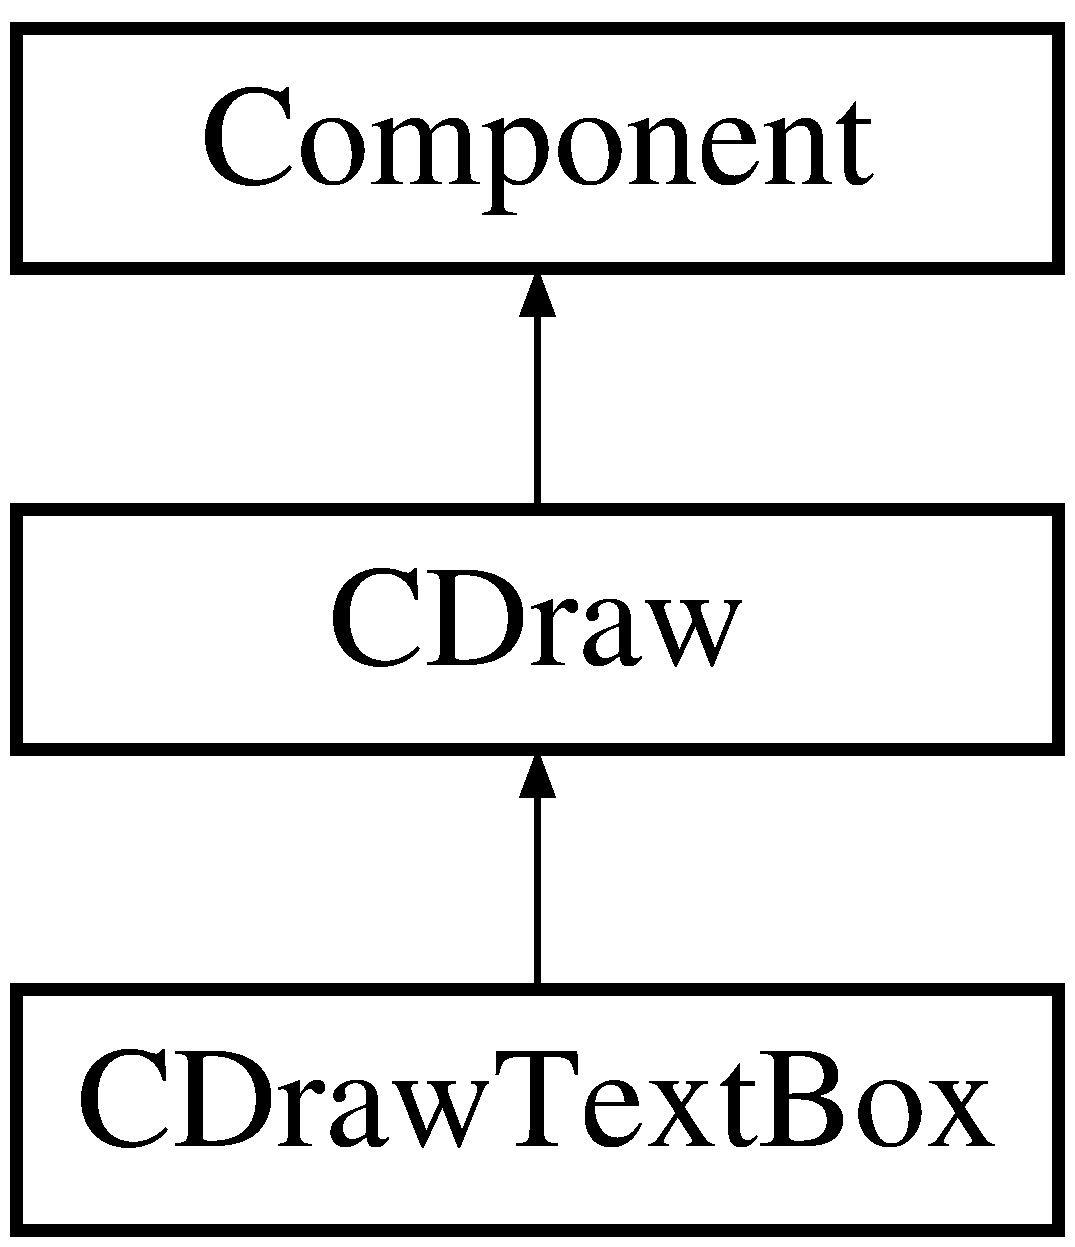
\includegraphics[height=3.000000cm]{class_c_draw_text_box}
\end{center}
\end{figure}
\subsection*{Public Member Functions}
\begin{DoxyCompactItemize}
\item 
\hypertarget{class_c_draw_text_box_aa2ba5a234bcd4e63bf7fbe7b10abd914}{}{\bfseries C\+Draw\+Text\+Box} (\hyperlink{class_s_render}{S\+Render} $\ast$\+\_\+o, \hyperlink{class_entity}{Entity} $\ast$\+\_\+e)\label{class_c_draw_text_box_aa2ba5a234bcd4e63bf7fbe7b10abd914}

\item 
\hypertarget{class_c_draw_text_box_acee17be5f109c79811e87e11c4281268}{}void {\bfseries init} ()\label{class_c_draw_text_box_acee17be5f109c79811e87e11c4281268}

\item 
\hypertarget{class_c_draw_text_box_a5e530639ce103a15abc92404b057e36f}{}void \hyperlink{class_c_draw_text_box_a5e530639ce103a15abc92404b057e36f}{draw} ()\label{class_c_draw_text_box_a5e530639ce103a15abc92404b057e36f}

\begin{DoxyCompactList}\small\item\em Affiche le champ texte. \end{DoxyCompactList}\item 
\hypertarget{class_c_draw_text_box_a8977b4095864ed28eaac326f8095e14e}{}void \hyperlink{class_c_draw_text_box_a8977b4095864ed28eaac326f8095e14e}{wordwrap} ()\label{class_c_draw_text_box_a8977b4095864ed28eaac326f8095e14e}

\begin{DoxyCompactList}\small\item\em Reviens à la ligne si le texte sort du cadre. \end{DoxyCompactList}\item 
\hypertarget{class_c_draw_text_box_a739e94ce36ce2c615806c3cdc8efe29d}{}bool \hyperlink{class_c_draw_text_box_a739e94ce36ce2c615806c3cdc8efe29d}{contains} (int, int)\label{class_c_draw_text_box_a739e94ce36ce2c615806c3cdc8efe29d}

\begin{DoxyCompactList}\small\item\em Check si les coordonées sont contenues dans le contenaire. \end{DoxyCompactList}\end{DoxyCompactItemize}
\subsection*{Additional Inherited Members}


\subsection{Detailed Description}
Classe héritant de \hyperlink{class_c_draw}{C\+Draw} et qui affiche un cadre et un texte. 

The documentation for this class was generated from the following files\+:\begin{DoxyCompactItemize}
\item 
component/\hyperlink{_c_draw_text_box_8hh}{C\+Draw\+Text\+Box.\+hh}\item 
component/C\+Draw\+Text\+Box.\+cpp\end{DoxyCompactItemize}

\hypertarget{class_c_draw_triangle}{}\section{C\+Draw\+Triangle Class Reference}
\label{class_c_draw_triangle}\index{C\+Draw\+Triangle@{C\+Draw\+Triangle}}


Classe héritant de \hyperlink{class_c_draw}{C\+Draw} et qui affiche un triangle.  




{\ttfamily \#include $<$C\+Draw\+Triangle.\+hh$>$}

Inheritance diagram for C\+Draw\+Triangle\+:\begin{figure}[H]
\begin{center}
\leavevmode
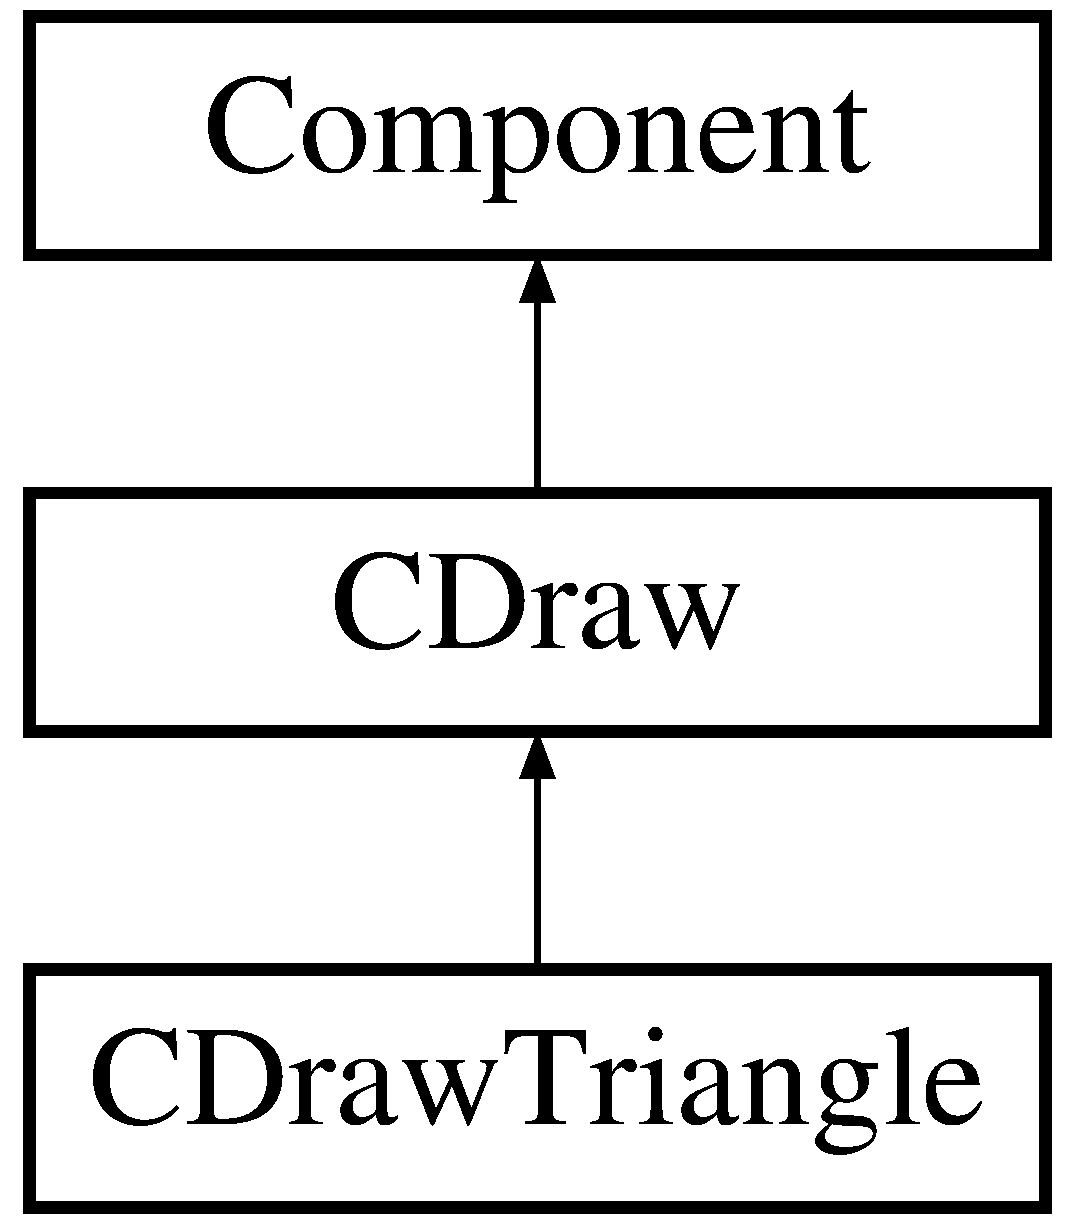
\includegraphics[height=3.000000cm]{class_c_draw_triangle}
\end{center}
\end{figure}
\subsection*{Public Member Functions}
\begin{DoxyCompactItemize}
\item 
\hypertarget{class_c_draw_triangle_abccc6d31eaa77adf1c8d972d10fdedc8}{}{\bfseries C\+Draw\+Triangle} (\hyperlink{class_s_render}{S\+Render} $\ast$\+\_\+o, \hyperlink{class_entity}{Entity} $\ast$\+\_\+e)\label{class_c_draw_triangle_abccc6d31eaa77adf1c8d972d10fdedc8}

\item 
\hypertarget{class_c_draw_triangle_adac4f1ef0652940baeb496f3a916437b}{}void \hyperlink{class_c_draw_triangle_adac4f1ef0652940baeb496f3a916437b}{draw} ()\label{class_c_draw_triangle_adac4f1ef0652940baeb496f3a916437b}

\begin{DoxyCompactList}\small\item\em Affiche le triangle. \end{DoxyCompactList}\item 
bool \hyperlink{class_c_draw_triangle_aedc4d96a23aad0355191a5fb55abc345}{contains} (int, int)
\begin{DoxyCompactList}\small\item\em Check si les coordonées sont contenues dans le triangle. \end{DoxyCompactList}\end{DoxyCompactItemize}
\subsection*{Additional Inherited Members}


\subsection{Detailed Description}
Classe héritant de \hyperlink{class_c_draw}{C\+Draw} et qui affiche un triangle. 

\subsection{Member Function Documentation}
\hypertarget{class_c_draw_triangle_aedc4d96a23aad0355191a5fb55abc345}{}\index{C\+Draw\+Triangle@{C\+Draw\+Triangle}!contains@{contains}}
\index{contains@{contains}!C\+Draw\+Triangle@{C\+Draw\+Triangle}}
\subsubsection[{contains}]{\setlength{\rightskip}{0pt plus 5cm}bool C\+Draw\+Triangle\+::contains (
\begin{DoxyParamCaption}
\item[{int}]{\+\_\+x, }
\item[{int}]{\+\_\+y}
\end{DoxyParamCaption}
)\hspace{0.3cm}{\ttfamily [virtual]}}\label{class_c_draw_triangle_aedc4d96a23aad0355191a5fb55abc345}


Check si les coordonées sont contenues dans le triangle. 

\begin{DoxyReturn}{Returns}
bool 
\end{DoxyReturn}


Implements \hyperlink{class_c_draw_a12c33a831c5a484f4173fbc385e63d72}{C\+Draw}.



The documentation for this class was generated from the following files\+:\begin{DoxyCompactItemize}
\item 
component/\hyperlink{_c_draw_triangle_8hh}{C\+Draw\+Triangle.\+hh}\item 
component/C\+Draw\+Triangle.\+cpp\end{DoxyCompactItemize}

\hypertarget{class_c_event}{}\section{C\+Event Class Reference}
\label{class_c_event}\index{C\+Event@{C\+Event}}


Classe héritant de \hyperlink{class_component}{Component} qui gère les Event.  




{\ttfamily \#include $<$C\+Event.\+hh$>$}

Inheritance diagram for C\+Event\+:\begin{figure}[H]
\begin{center}
\leavevmode
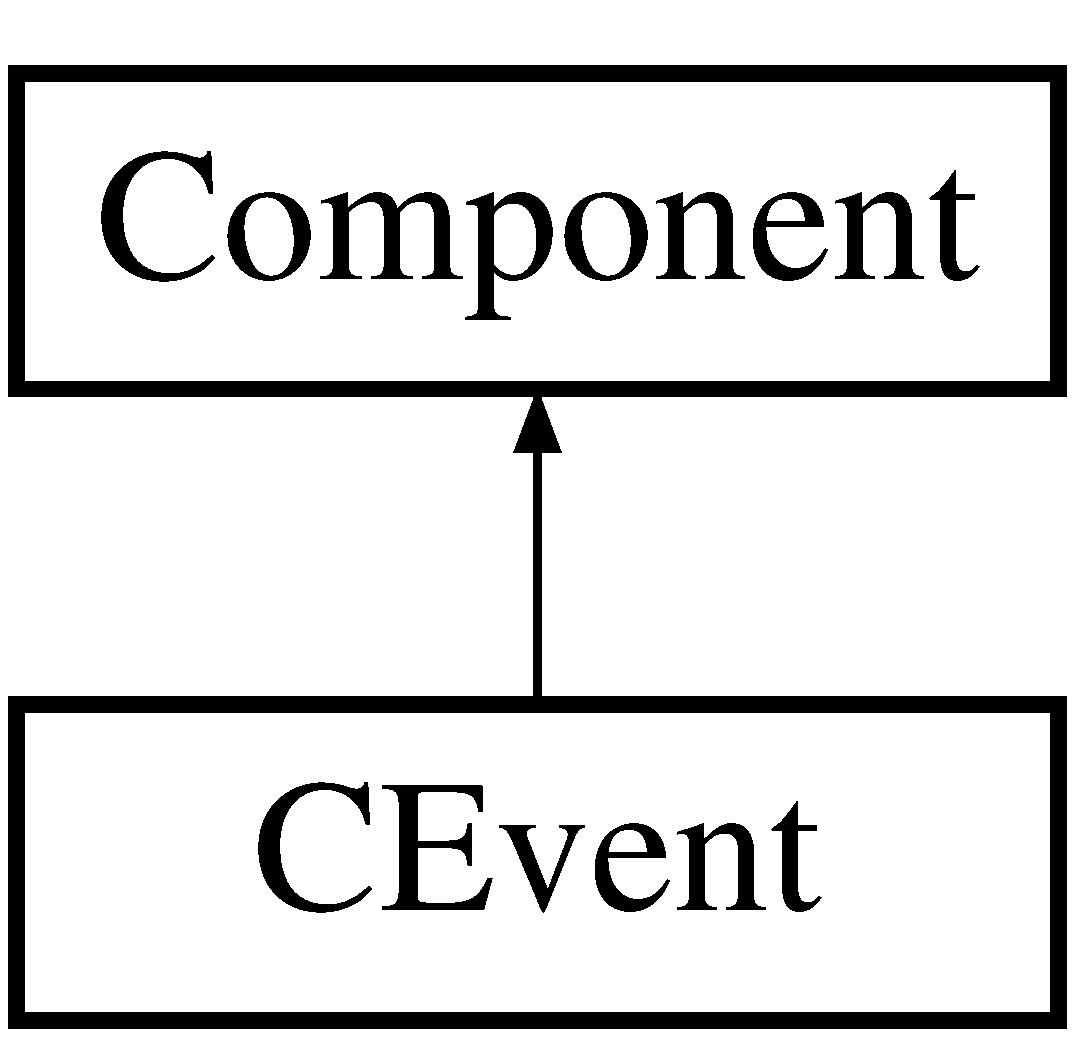
\includegraphics[height=2.000000cm]{class_c_event}
\end{center}
\end{figure}
\subsection*{Public Member Functions}
\begin{DoxyCompactItemize}
\item 
\hypertarget{class_c_event_a85be8a946bcaf5b2bae52126d9804d16}{}{\bfseries C\+Event} (\hyperlink{class_s_render}{S\+Render} $\ast$, \hyperlink{class_entity}{Entity} $\ast$)\label{class_c_event_a85be8a946bcaf5b2bae52126d9804d16}

\item 
\hyperlink{class_c_event}{C\+Event} $\ast$ \hyperlink{class_c_event_ad43296e11915e550761216b4866f2b75}{set\+Event} (sf\+::\+Event\+::\+Event\+Type, void($\ast$)(\hyperlink{class_entity}{Entity} $\ast$, sf\+::\+Event \&))
\begin{DoxyCompactList}\small\item\em Spécifie une réaction par rapport à un évenement. \end{DoxyCompactList}\item 
\hyperlink{class_c_event}{C\+Event} $\ast$ \hyperlink{class_c_event_a51534e6480051b3b2c38f618c27495cb}{receive\+Event} (sf\+::\+Event \&)
\begin{DoxyCompactList}\small\item\em Reçois un évenement et appelle la fonction correspondante. $\ast$. \end{DoxyCompactList}\item 
\hyperlink{class_c_event}{C\+Event} $\ast$ \hyperlink{class_c_event_a027b94f30ebdf2f699613aa56570ea86}{check\+Event} (sf\+::\+Event \&)
\begin{DoxyCompactList}\small\item\em Reçois un évenement et vérifie si il devient le focus, si il doit réagir. \end{DoxyCompactList}\item 
\hypertarget{class_c_event_ae9c23f7c6cc4db8502790ff10c6a0c32}{}void \hyperlink{class_c_event_ae9c23f7c6cc4db8502790ff10c6a0c32}{propagate\+Children} (sf\+::\+Event \&)\label{class_c_event_ae9c23f7c6cc4db8502790ff10c6a0c32}

\begin{DoxyCompactList}\small\item\em Propage l\textquotesingle{}évenement aux enfants. \end{DoxyCompactList}\end{DoxyCompactItemize}
\subsection*{Additional Inherited Members}


\subsection{Detailed Description}
Classe héritant de \hyperlink{class_component}{Component} qui gère les Event. 

La classe possède un pointeur sur le \hyperlink{class_s_render}{S\+Render} et sur l\textquotesingle{}entity ainsi qu\textquotesingle{}un tableau de pointeur sur fonction indexé par Event\+Type.

Les fonctions doivent respecter ce prototype void fct(\+Entity $\ast$, sf\+::\+Event \&) Elles recevront en premier paramètre l\textquotesingle{}entitée et en deuxième paramètre l\textquotesingle{}event S\+F\+M\+L 

\subsection{Member Function Documentation}
\hypertarget{class_c_event_a027b94f30ebdf2f699613aa56570ea86}{}\index{C\+Event@{C\+Event}!check\+Event@{check\+Event}}
\index{check\+Event@{check\+Event}!C\+Event@{C\+Event}}
\subsubsection[{check\+Event}]{\setlength{\rightskip}{0pt plus 5cm}{\bf C\+Event} $\ast$ C\+Event\+::check\+Event (
\begin{DoxyParamCaption}
\item[{sf\+::\+Event \&}]{event}
\end{DoxyParamCaption}
)}\label{class_c_event_a027b94f30ebdf2f699613aa56570ea86}


Reçois un évenement et vérifie si il devient le focus, si il doit réagir. 

\begin{DoxyReturn}{Returns}
\hyperlink{class_c_event}{C\+Event} $\ast$ 
\end{DoxyReturn}
\hypertarget{class_c_event_a51534e6480051b3b2c38f618c27495cb}{}\index{C\+Event@{C\+Event}!receive\+Event@{receive\+Event}}
\index{receive\+Event@{receive\+Event}!C\+Event@{C\+Event}}
\subsubsection[{receive\+Event}]{\setlength{\rightskip}{0pt plus 5cm}{\bf C\+Event} $\ast$ C\+Event\+::receive\+Event (
\begin{DoxyParamCaption}
\item[{sf\+::\+Event \&}]{event}
\end{DoxyParamCaption}
)}\label{class_c_event_a51534e6480051b3b2c38f618c27495cb}


Reçois un évenement et appelle la fonction correspondante. $\ast$. 

\begin{DoxyReturn}{Returns}
\hyperlink{class_c_event}{C\+Event} $\ast$ 
\end{DoxyReturn}
\hypertarget{class_c_event_ad43296e11915e550761216b4866f2b75}{}\index{C\+Event@{C\+Event}!set\+Event@{set\+Event}}
\index{set\+Event@{set\+Event}!C\+Event@{C\+Event}}
\subsubsection[{set\+Event}]{\setlength{\rightskip}{0pt plus 5cm}{\bf C\+Event} $\ast$ C\+Event\+::set\+Event (
\begin{DoxyParamCaption}
\item[{sf\+::\+Event\+::\+Event\+Type}]{ev, }
\item[{void($\ast$)({\bf Entity} $\ast$, sf\+::\+Event \&)}]{fct}
\end{DoxyParamCaption}
)}\label{class_c_event_ad43296e11915e550761216b4866f2b75}


Spécifie une réaction par rapport à un évenement. 

\begin{DoxyReturn}{Returns}
\hyperlink{class_c_event}{C\+Event} $\ast$ 
\end{DoxyReturn}


The documentation for this class was generated from the following files\+:\begin{DoxyCompactItemize}
\item 
component/\hyperlink{_c_event_8hh}{C\+Event.\+hh}\item 
component/C\+Event.\+cpp\end{DoxyCompactItemize}

\hypertarget{class_c_geometry}{}\section{C\+Geometry Class Reference}
\label{class_c_geometry}\index{C\+Geometry@{C\+Geometry}}


Classe héritant de \hyperlink{class_component}{Component}.  




{\ttfamily \#include $<$C\+Geometry.\+hh$>$}

Inheritance diagram for C\+Geometry\+:\begin{figure}[H]
\begin{center}
\leavevmode
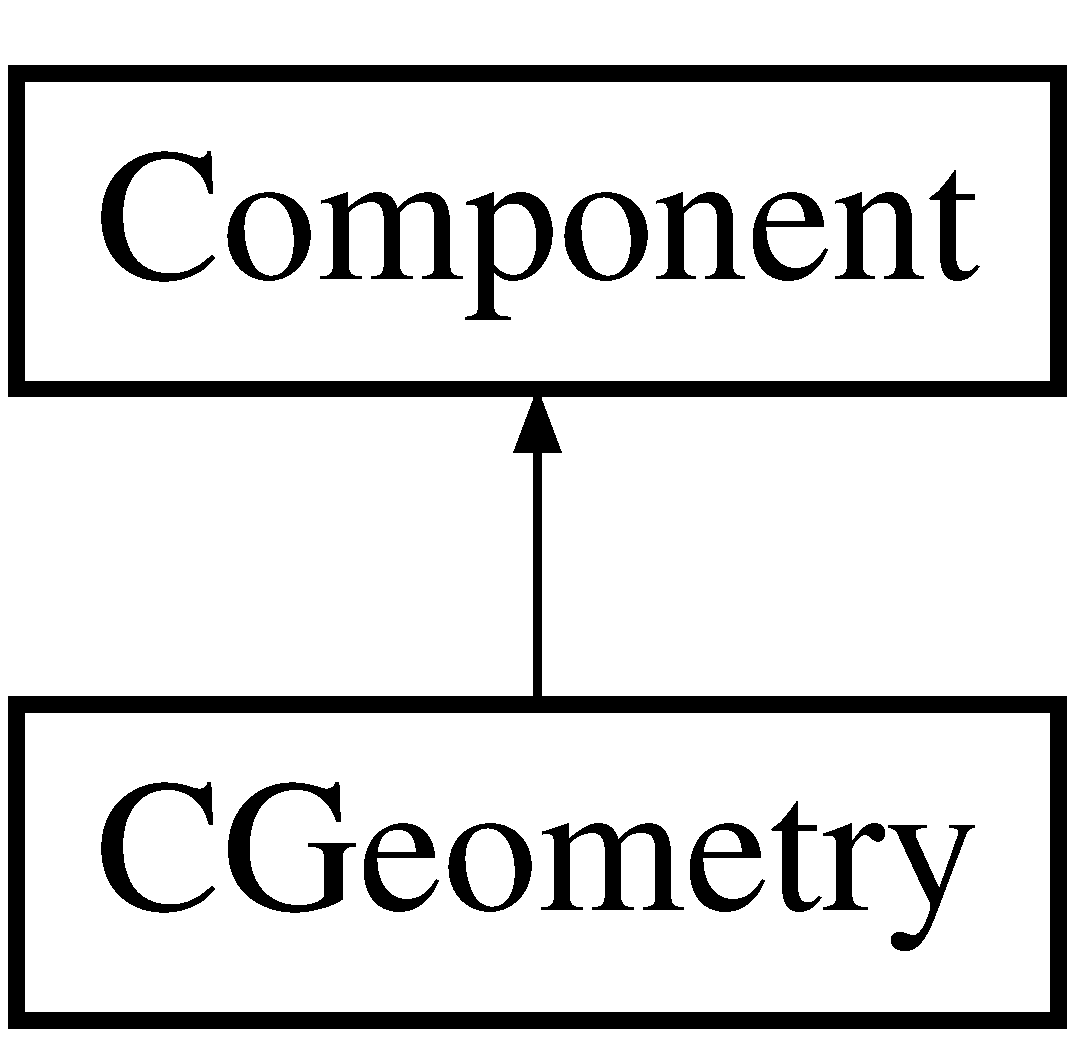
\includegraphics[height=2.000000cm]{class_c_geometry}
\end{center}
\end{figure}
\subsection*{Public Member Functions}
\begin{DoxyCompactItemize}
\item 
int \hyperlink{class_c_geometry_a1ef1162bc64762d26a69941fee616d93}{get} (const std\+::string \&)
\begin{DoxyCompactList}\small\item\em Récupère une donnée à partir de son nom en string. \end{DoxyCompactList}\item 
data\+\_\+map \& \hyperlink{class_c_geometry_a688f5db2b2a76f7b0bf6e4507769a838}{get\+Data} ()
\begin{DoxyCompactList}\small\item\em Récupère l\textquotesingle{}ensemble des données. \end{DoxyCompactList}\item 
\hyperlink{class_c_geometry}{C\+Geometry} $\ast$ \hyperlink{class_c_geometry_ac4da7f8f7cc75a51fde473f36b0e45b2}{set} (const std\+::string \&, int)
\begin{DoxyCompactList}\small\item\em Assigne la valeur à la clé correspondante. \end{DoxyCompactList}\item 
\hyperlink{class_c_geometry}{C\+Geometry} $\ast$ \hyperlink{class_c_geometry_a005ba0235bea89dc99f4168e8d601529}{set\+Data} (const data\+\_\+map \&)
\begin{DoxyCompactList}\small\item\em Assigne toute une map. \end{DoxyCompactList}\item 
\hyperlink{class_c_geometry}{C\+Geometry} $\ast$ \hyperlink{class_c_geometry_aa5b2f21b9f0f8ca71adac95deb83c988}{add} (const std\+::string \&, int)
\begin{DoxyCompactList}\small\item\em Ajoute à la valeur de la clé. \end{DoxyCompactList}\item 
\hyperlink{class_c_geometry}{C\+Geometry} $\ast$ \hyperlink{class_c_geometry_a4ecf6f7759dc70dc0dd04b9a68db8c1b}{substract} (const std\+::string \&, int)
\begin{DoxyCompactList}\small\item\em Soustrait à la valeur de la clé. \end{DoxyCompactList}\item 
\hyperlink{class_c_geometry}{C\+Geometry} $\ast$ \hyperlink{class_c_geometry_a12e0bb0758ad8ae8b03810acf43679f9}{multiply} (const std\+::string \&, int)
\begin{DoxyCompactList}\small\item\em Multiplie la valeur de la clé. \end{DoxyCompactList}\item 
\hyperlink{class_c_geometry}{C\+Geometry} $\ast$ \hyperlink{class_c_geometry_a960106ec0217d6b89cdbfe5b9f8028be}{divides} (const std\+::string \&, int)
\begin{DoxyCompactList}\small\item\em Divise la valeur de la clé. \end{DoxyCompactList}\end{DoxyCompactItemize}
\subsection*{Additional Inherited Members}


\subsection{Detailed Description}
Classe héritant de \hyperlink{class_component}{Component}. 

\subsection{Member Function Documentation}
\hypertarget{class_c_geometry_aa5b2f21b9f0f8ca71adac95deb83c988}{}\index{C\+Geometry@{C\+Geometry}!add@{add}}
\index{add@{add}!C\+Geometry@{C\+Geometry}}
\subsubsection[{add}]{\setlength{\rightskip}{0pt plus 5cm}{\bf C\+Geometry} $\ast$ C\+Geometry\+::add (
\begin{DoxyParamCaption}
\item[{const std\+::string \&}]{key, }
\item[{int}]{value}
\end{DoxyParamCaption}
)}\label{class_c_geometry_aa5b2f21b9f0f8ca71adac95deb83c988}


Ajoute à la valeur de la clé. 

\begin{DoxyReturn}{Returns}
\hyperlink{class_c_geometry}{C\+Geometry} $\ast$this 
\end{DoxyReturn}
\hypertarget{class_c_geometry_a960106ec0217d6b89cdbfe5b9f8028be}{}\index{C\+Geometry@{C\+Geometry}!divides@{divides}}
\index{divides@{divides}!C\+Geometry@{C\+Geometry}}
\subsubsection[{divides}]{\setlength{\rightskip}{0pt plus 5cm}{\bf C\+Geometry} $\ast$ C\+Geometry\+::divides (
\begin{DoxyParamCaption}
\item[{const std\+::string \&}]{key, }
\item[{int}]{value}
\end{DoxyParamCaption}
)}\label{class_c_geometry_a960106ec0217d6b89cdbfe5b9f8028be}


Divise la valeur de la clé. 

\begin{DoxyReturn}{Returns}
\hyperlink{class_c_geometry}{C\+Geometry} $\ast$this 
\end{DoxyReturn}
\hypertarget{class_c_geometry_a1ef1162bc64762d26a69941fee616d93}{}\index{C\+Geometry@{C\+Geometry}!get@{get}}
\index{get@{get}!C\+Geometry@{C\+Geometry}}
\subsubsection[{get}]{\setlength{\rightskip}{0pt plus 5cm}int C\+Geometry\+::get (
\begin{DoxyParamCaption}
\item[{const std\+::string \&}]{key}
\end{DoxyParamCaption}
)}\label{class_c_geometry_a1ef1162bc64762d26a69941fee616d93}


Récupère une donnée à partir de son nom en string. 

\begin{DoxyReturn}{Returns}
int value 
\end{DoxyReturn}
\hypertarget{class_c_geometry_a688f5db2b2a76f7b0bf6e4507769a838}{}\index{C\+Geometry@{C\+Geometry}!get\+Data@{get\+Data}}
\index{get\+Data@{get\+Data}!C\+Geometry@{C\+Geometry}}
\subsubsection[{get\+Data}]{\setlength{\rightskip}{0pt plus 5cm}data\+\_\+map \& C\+Geometry\+::get\+Data (
\begin{DoxyParamCaption}
{}
\end{DoxyParamCaption}
)}\label{class_c_geometry_a688f5db2b2a76f7b0bf6e4507769a838}


Récupère l\textquotesingle{}ensemble des données. 

\begin{DoxyReturn}{Returns}
data\+\_\+map data 
\end{DoxyReturn}
\hypertarget{class_c_geometry_a12e0bb0758ad8ae8b03810acf43679f9}{}\index{C\+Geometry@{C\+Geometry}!multiply@{multiply}}
\index{multiply@{multiply}!C\+Geometry@{C\+Geometry}}
\subsubsection[{multiply}]{\setlength{\rightskip}{0pt plus 5cm}{\bf C\+Geometry} $\ast$ C\+Geometry\+::multiply (
\begin{DoxyParamCaption}
\item[{const std\+::string \&}]{key, }
\item[{int}]{value}
\end{DoxyParamCaption}
)}\label{class_c_geometry_a12e0bb0758ad8ae8b03810acf43679f9}


Multiplie la valeur de la clé. 

\begin{DoxyReturn}{Returns}
\hyperlink{class_c_geometry}{C\+Geometry} $\ast$this 
\end{DoxyReturn}
\hypertarget{class_c_geometry_ac4da7f8f7cc75a51fde473f36b0e45b2}{}\index{C\+Geometry@{C\+Geometry}!set@{set}}
\index{set@{set}!C\+Geometry@{C\+Geometry}}
\subsubsection[{set}]{\setlength{\rightskip}{0pt plus 5cm}{\bf C\+Geometry} $\ast$ C\+Geometry\+::set (
\begin{DoxyParamCaption}
\item[{const std\+::string \&}]{key, }
\item[{int}]{value}
\end{DoxyParamCaption}
)}\label{class_c_geometry_ac4da7f8f7cc75a51fde473f36b0e45b2}


Assigne la valeur à la clé correspondante. 

\begin{DoxyReturn}{Returns}
\hyperlink{class_c_geometry}{C\+Geometry} $\ast$this 
\end{DoxyReturn}
\hypertarget{class_c_geometry_a005ba0235bea89dc99f4168e8d601529}{}\index{C\+Geometry@{C\+Geometry}!set\+Data@{set\+Data}}
\index{set\+Data@{set\+Data}!C\+Geometry@{C\+Geometry}}
\subsubsection[{set\+Data}]{\setlength{\rightskip}{0pt plus 5cm}{\bf C\+Geometry} $\ast$ C\+Geometry\+::set\+Data (
\begin{DoxyParamCaption}
\item[{const data\+\_\+map \&}]{setted\+Map}
\end{DoxyParamCaption}
)}\label{class_c_geometry_a005ba0235bea89dc99f4168e8d601529}


Assigne toute une map. 

\begin{DoxyReturn}{Returns}
\hyperlink{class_c_geometry}{C\+Geometry} $\ast$this 
\end{DoxyReturn}
\hypertarget{class_c_geometry_a4ecf6f7759dc70dc0dd04b9a68db8c1b}{}\index{C\+Geometry@{C\+Geometry}!substract@{substract}}
\index{substract@{substract}!C\+Geometry@{C\+Geometry}}
\subsubsection[{substract}]{\setlength{\rightskip}{0pt plus 5cm}{\bf C\+Geometry} $\ast$ C\+Geometry\+::substract (
\begin{DoxyParamCaption}
\item[{const std\+::string \&}]{key, }
\item[{int}]{value}
\end{DoxyParamCaption}
)}\label{class_c_geometry_a4ecf6f7759dc70dc0dd04b9a68db8c1b}


Soustrait à la valeur de la clé. 

\begin{DoxyReturn}{Returns}
\hyperlink{class_c_geometry}{C\+Geometry} $\ast$this 
\end{DoxyReturn}


The documentation for this class was generated from the following files\+:\begin{DoxyCompactItemize}
\item 
component/\hyperlink{_c_geometry_8hh}{C\+Geometry.\+hh}\item 
component/C\+Geometry.\+cpp\end{DoxyCompactItemize}

\hypertarget{class_c_identifier}{}\section{C\+Identifier Class Reference}
\label{class_c_identifier}\index{C\+Identifier@{C\+Identifier}}


Classe héritant de \hyperlink{class_component}{Component} stockant l\textquotesingle{}id.  




{\ttfamily \#include $<$C\+Identifier.\+hh$>$}

Inheritance diagram for C\+Identifier\+:\begin{figure}[H]
\begin{center}
\leavevmode
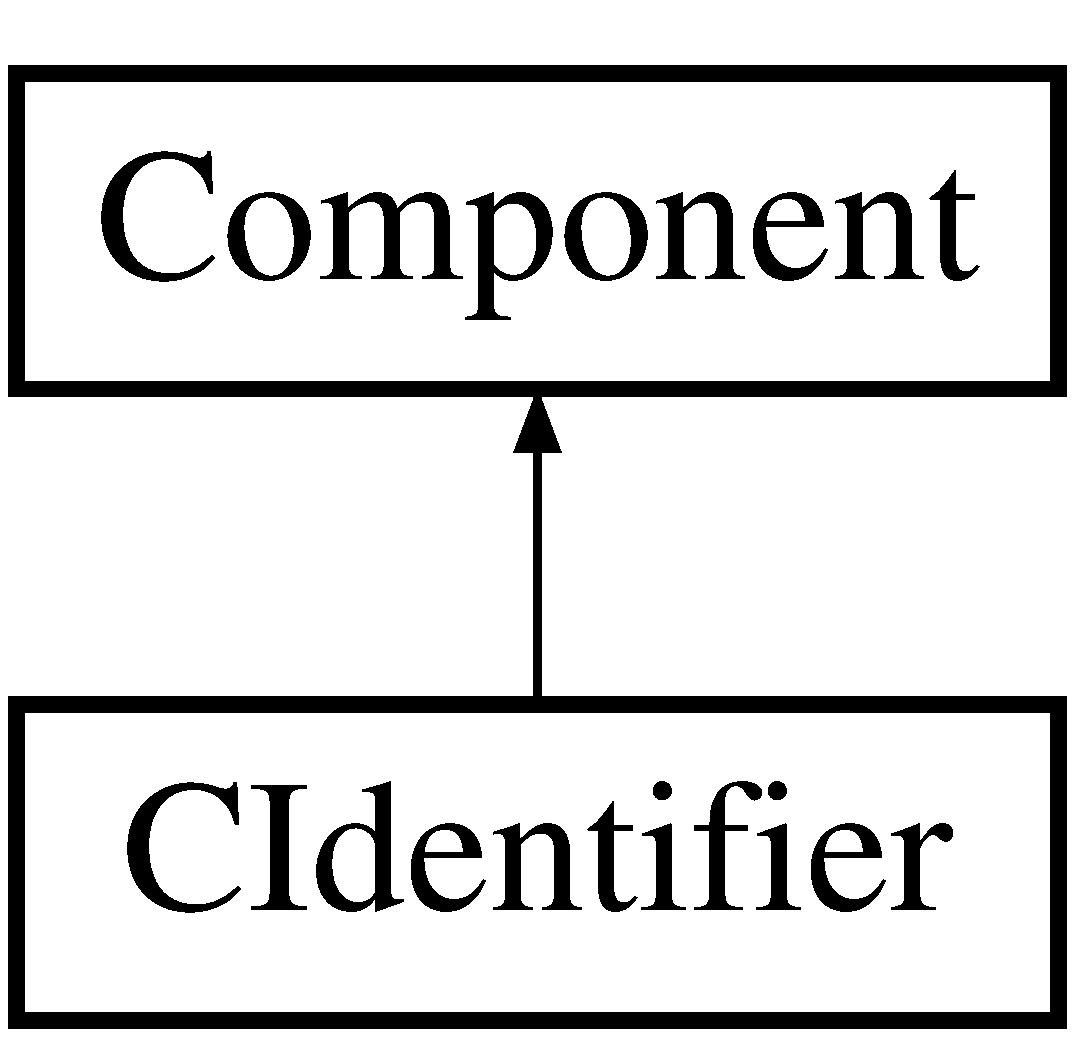
\includegraphics[height=2.000000cm]{class_c_identifier}
\end{center}
\end{figure}
\subsection*{Public Member Functions}
\begin{DoxyCompactItemize}
\item 
\hyperlink{class_c_identifier}{C\+Identifier} $\ast$ \hyperlink{class_c_identifier_a0b0e4bef79c2ae06659166b8acf3fc4c}{set\+Id} (int)
\begin{DoxyCompactList}\small\item\em Assigne une I\+D. \end{DoxyCompactList}\item 
int \hyperlink{class_c_identifier_aa7ca7f565792853d3e41c3b9c04aa193}{get\+Id} ()
\begin{DoxyCompactList}\small\item\em Récupère une I\+D. \end{DoxyCompactList}\end{DoxyCompactItemize}
\subsection*{Additional Inherited Members}


\subsection{Detailed Description}
Classe héritant de \hyperlink{class_component}{Component} stockant l\textquotesingle{}id. 

\subsection{Member Function Documentation}
\hypertarget{class_c_identifier_aa7ca7f565792853d3e41c3b9c04aa193}{}\index{C\+Identifier@{C\+Identifier}!get\+Id@{get\+Id}}
\index{get\+Id@{get\+Id}!C\+Identifier@{C\+Identifier}}
\subsubsection[{get\+Id}]{\setlength{\rightskip}{0pt plus 5cm}int C\+Identifier\+::get\+Id (
\begin{DoxyParamCaption}
{}
\end{DoxyParamCaption}
)}\label{class_c_identifier_aa7ca7f565792853d3e41c3b9c04aa193}


Récupère une I\+D. 

\begin{DoxyReturn}{Returns}
int id 
\end{DoxyReturn}
\hypertarget{class_c_identifier_a0b0e4bef79c2ae06659166b8acf3fc4c}{}\index{C\+Identifier@{C\+Identifier}!set\+Id@{set\+Id}}
\index{set\+Id@{set\+Id}!C\+Identifier@{C\+Identifier}}
\subsubsection[{set\+Id}]{\setlength{\rightskip}{0pt plus 5cm}{\bf C\+Identifier} $\ast$ C\+Identifier\+::set\+Id (
\begin{DoxyParamCaption}
\item[{int}]{\+\_\+id}
\end{DoxyParamCaption}
)}\label{class_c_identifier_a0b0e4bef79c2ae06659166b8acf3fc4c}


Assigne une I\+D. 

\begin{DoxyReturn}{Returns}
\hyperlink{class_c_identifier}{C\+Identifier} $\ast$this 
\end{DoxyReturn}


The documentation for this class was generated from the following files\+:\begin{DoxyCompactItemize}
\item 
component/\hyperlink{_c_identifier_8hh}{C\+Identifier.\+hh}\item 
component/C\+Identifier.\+cpp\end{DoxyCompactItemize}

\hypertarget{class_c_label}{}\section{C\+Label Class Reference}
\label{class_c_label}\index{C\+Label@{C\+Label}}


Classe héritant de \hyperlink{class_component}{Component} contient le label en string et le fontsize en int.  




{\ttfamily \#include $<$C\+Label.\+hh$>$}

Inheritance diagram for C\+Label\+:\begin{figure}[H]
\begin{center}
\leavevmode
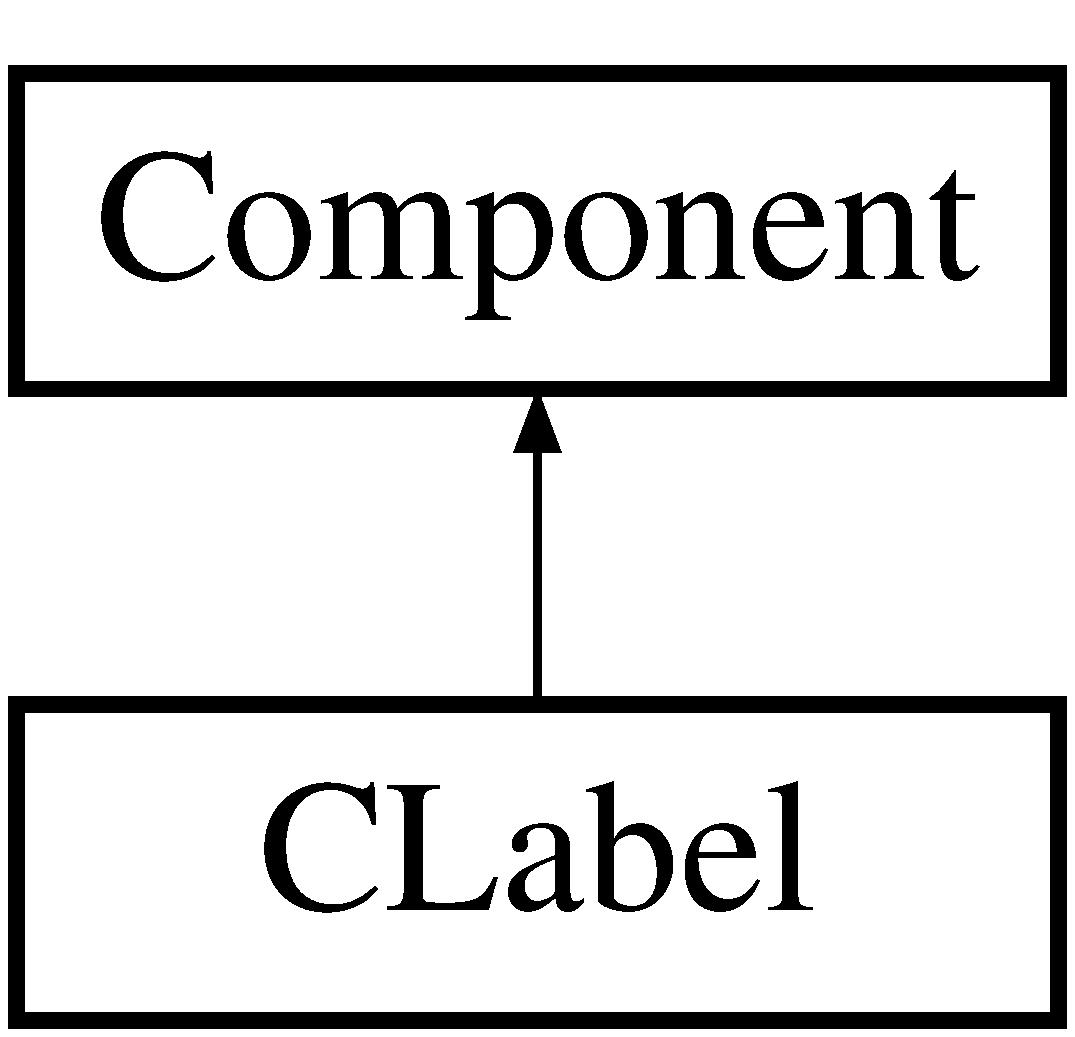
\includegraphics[height=2.000000cm]{class_c_label}
\end{center}
\end{figure}
\subsection*{Public Member Functions}
\begin{DoxyCompactItemize}
\item 
\hyperlink{class_c_label}{C\+Label} $\ast$ \hyperlink{class_c_label_a8b75f2c74e64b9a4453ab8adc839e16f}{set\+Label} (const std\+::string \&)
\begin{DoxyCompactList}\small\item\em Assigne un label à l\textquotesingle{}entité \end{DoxyCompactList}\item 
const std\+::string \& \hyperlink{class_c_label_a3bdb26bfcb7cf8801340e46240cbf2a5}{get\+Label} ()
\begin{DoxyCompactList}\small\item\em Récupère le label de l\textquotesingle{}entité \end{DoxyCompactList}\item 
\hyperlink{class_c_label}{C\+Label} $\ast$ \hyperlink{class_c_label_a69a80521075af5e41222038cf536af0f}{set\+Font\+Size} (int)
\begin{DoxyCompactList}\small\item\em Assigne une taille de police au label. \end{DoxyCompactList}\item 
int \hyperlink{class_c_label_a11d5ce9578dbd1fd8c88423f8da7617a}{get\+Font\+Size} ()
\begin{DoxyCompactList}\small\item\em Récupère la tailel de police. \end{DoxyCompactList}\end{DoxyCompactItemize}
\subsection*{Additional Inherited Members}


\subsection{Detailed Description}
Classe héritant de \hyperlink{class_component}{Component} contient le label en string et le fontsize en int. 

\subsection{Member Function Documentation}
\hypertarget{class_c_label_a11d5ce9578dbd1fd8c88423f8da7617a}{}\index{C\+Label@{C\+Label}!get\+Font\+Size@{get\+Font\+Size}}
\index{get\+Font\+Size@{get\+Font\+Size}!C\+Label@{C\+Label}}
\subsubsection[{get\+Font\+Size}]{\setlength{\rightskip}{0pt plus 5cm}int C\+Label\+::get\+Font\+Size (
\begin{DoxyParamCaption}
{}
\end{DoxyParamCaption}
)}\label{class_c_label_a11d5ce9578dbd1fd8c88423f8da7617a}


Récupère la tailel de police. 

\begin{DoxyReturn}{Returns}
int 
\end{DoxyReturn}
\hypertarget{class_c_label_a3bdb26bfcb7cf8801340e46240cbf2a5}{}\index{C\+Label@{C\+Label}!get\+Label@{get\+Label}}
\index{get\+Label@{get\+Label}!C\+Label@{C\+Label}}
\subsubsection[{get\+Label}]{\setlength{\rightskip}{0pt plus 5cm}const std\+::string \& C\+Label\+::get\+Label (
\begin{DoxyParamCaption}
{}
\end{DoxyParamCaption}
)}\label{class_c_label_a3bdb26bfcb7cf8801340e46240cbf2a5}


Récupère le label de l\textquotesingle{}entité 

\begin{DoxyReturn}{Returns}
const std\+::string \&label 
\end{DoxyReturn}
\hypertarget{class_c_label_a69a80521075af5e41222038cf536af0f}{}\index{C\+Label@{C\+Label}!set\+Font\+Size@{set\+Font\+Size}}
\index{set\+Font\+Size@{set\+Font\+Size}!C\+Label@{C\+Label}}
\subsubsection[{set\+Font\+Size}]{\setlength{\rightskip}{0pt plus 5cm}{\bf C\+Label} $\ast$ C\+Label\+::set\+Font\+Size (
\begin{DoxyParamCaption}
\item[{int}]{\+\_\+font\+Size}
\end{DoxyParamCaption}
)}\label{class_c_label_a69a80521075af5e41222038cf536af0f}


Assigne une taille de police au label. 

\begin{DoxyReturn}{Returns}
\hyperlink{class_c_label}{C\+Label} $\ast$this 
\end{DoxyReturn}
\hypertarget{class_c_label_a8b75f2c74e64b9a4453ab8adc839e16f}{}\index{C\+Label@{C\+Label}!set\+Label@{set\+Label}}
\index{set\+Label@{set\+Label}!C\+Label@{C\+Label}}
\subsubsection[{set\+Label}]{\setlength{\rightskip}{0pt plus 5cm}{\bf C\+Label} $\ast$ C\+Label\+::set\+Label (
\begin{DoxyParamCaption}
\item[{const std\+::string \&}]{\+\_\+label}
\end{DoxyParamCaption}
)}\label{class_c_label_a8b75f2c74e64b9a4453ab8adc839e16f}


Assigne un label à l\textquotesingle{}entité 

\begin{DoxyReturn}{Returns}
\hyperlink{class_c_label}{C\+Label} $\ast$this 
\end{DoxyReturn}


The documentation for this class was generated from the following files\+:\begin{DoxyCompactItemize}
\item 
component/\hyperlink{_c_label_8hh}{C\+Label.\+hh}\item 
component/C\+Label.\+cpp\end{DoxyCompactItemize}

\hypertarget{class_component}{}\section{Component Class Reference}
\label{class_component}\index{Component@{Component}}


Parent de tous les components.  




{\ttfamily \#include $<$Component.\+hh$>$}

Inheritance diagram for Component\+:\begin{figure}[H]
\begin{center}
\leavevmode
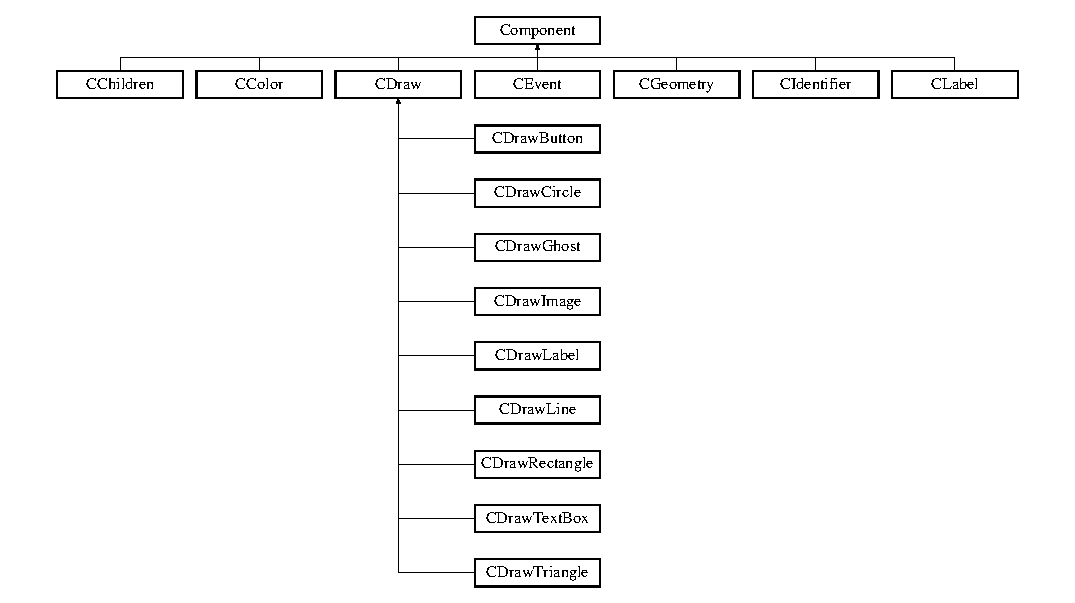
\includegraphics[height=7.652174cm]{class_component}
\end{center}
\end{figure}
\subsection*{Public Member Functions}
\begin{DoxyCompactItemize}
\item 
bool \hyperlink{class_component_a9f4ff1993db2a1694fabd7bd6e63af2a}{has\+Change} ()
\begin{DoxyCompactList}\small\item\em Renvoie la value de change. \end{DoxyCompactList}\end{DoxyCompactItemize}
\subsection*{Protected Attributes}
\begin{DoxyCompactItemize}
\item 
\hypertarget{class_component_a0f4af849e74141ff37e0bae44a667269}{}bool {\bfseries change}\label{class_component_a0f4af849e74141ff37e0bae44a667269}

\end{DoxyCompactItemize}


\subsection{Detailed Description}
Parent de tous les components. 

En plus de permettre de stocker tous les components au meme endroit \hyperlink{class_component}{Component} contient aussi un boolean qui permet de savoir si un changement a été effectué. 

\subsection{Member Function Documentation}
\hypertarget{class_component_a9f4ff1993db2a1694fabd7bd6e63af2a}{}\index{Component@{Component}!has\+Change@{has\+Change}}
\index{has\+Change@{has\+Change}!Component@{Component}}
\subsubsection[{has\+Change}]{\setlength{\rightskip}{0pt plus 5cm}bool Component\+::has\+Change (
\begin{DoxyParamCaption}
{}
\end{DoxyParamCaption}
)}\label{class_component_a9f4ff1993db2a1694fabd7bd6e63af2a}


Renvoie la value de change. 

Si un changement a été effectué change est mis à true. la fonction renverra ainsi true si nécéssaire et passera le change à false le changement ayant bien été notifié.

\begin{DoxyReturn}{Returns}
boolean change 
\end{DoxyReturn}


The documentation for this class was generated from the following files\+:\begin{DoxyCompactItemize}
\item 
component/\hyperlink{_component_8hh}{Component.\+hh}\item 
component/Component.\+cpp\end{DoxyCompactItemize}

\hypertarget{class_entity}{}\section{Entity Class Reference}
\label{class_entity}\index{Entity@{Entity}}


Classe possédant une map de component et gérant les accès.  




{\ttfamily \#include $<$Entity.\+hh$>$}

\subsection*{Public Member Functions}
\begin{DoxyCompactItemize}
\item 
{\footnotesize template$<$typename T $>$ }\\T $\ast$ \hyperlink{class_entity_ab1565dea579b29e0431a9d1c106d8e34}{set\+Attr} ()
\begin{DoxyCompactList}\small\item\em Crée un component. \end{DoxyCompactList}\item 
{\footnotesize template$<$typename T $>$ }\\T \hyperlink{class_entity_afb39788bb9d49672d59ae6d367e7f6b2}{set\+Attr} (\hyperlink{class_component}{Component} $\ast$c)
\begin{DoxyCompactList}\small\item\em Assigne un component. \end{DoxyCompactList}\item 
{\footnotesize template$<$typename T $>$ }\\T \hyperlink{class_entity_a71c7f216536c0af004c0c62b0c2ceb3b}{get\+Attr} ()
\begin{DoxyCompactList}\small\item\em Récupère un component. \end{DoxyCompactList}\end{DoxyCompactItemize}


\subsection{Detailed Description}
Classe possédant une map de component et gérant les accès. 

La component\+\_\+map est faite de Component$\ast$ indexé par l\textquotesingle{}Id de leur classe 

\subsection{Member Function Documentation}
\hypertarget{class_entity_a71c7f216536c0af004c0c62b0c2ceb3b}{}\index{Entity@{Entity}!get\+Attr@{get\+Attr}}
\index{get\+Attr@{get\+Attr}!Entity@{Entity}}
\subsubsection[{get\+Attr}]{\setlength{\rightskip}{0pt plus 5cm}template$<$typename T $>$ T Entity\+::get\+Attr (
\begin{DoxyParamCaption}
{}
\end{DoxyParamCaption}
)\hspace{0.3cm}{\ttfamily [inline]}}\label{class_entity_a71c7f216536c0af004c0c62b0c2ceb3b}


Récupère un component. 

Renvoie le component de la classe passé en template en se servant de son id de classe. Effectue un cast pour passer de \hyperlink{class_component}{Component} $\ast$ à T. \begin{DoxyReturn}{Returns}
T component 
\end{DoxyReturn}
\hypertarget{class_entity_ab1565dea579b29e0431a9d1c106d8e34}{}\index{Entity@{Entity}!set\+Attr@{set\+Attr}}
\index{set\+Attr@{set\+Attr}!Entity@{Entity}}
\subsubsection[{set\+Attr}]{\setlength{\rightskip}{0pt plus 5cm}template$<$typename T $>$ T$\ast$ Entity\+::set\+Attr (
\begin{DoxyParamCaption}
{}
\end{DoxyParamCaption}
)\hspace{0.3cm}{\ttfamily [inline]}}\label{class_entity_ab1565dea579b29e0431a9d1c106d8e34}


Crée un component. 

Ajoute le component passé en template à la map avec comme clé L\textquotesingle{}id de la classe du component Effectue un cast du component créé et le return \begin{DoxyReturn}{Returns}
T $\ast$component 
\end{DoxyReturn}
\hypertarget{class_entity_afb39788bb9d49672d59ae6d367e7f6b2}{}\index{Entity@{Entity}!set\+Attr@{set\+Attr}}
\index{set\+Attr@{set\+Attr}!Entity@{Entity}}
\subsubsection[{set\+Attr}]{\setlength{\rightskip}{0pt plus 5cm}template$<$typename T $>$ T Entity\+::set\+Attr (
\begin{DoxyParamCaption}
\item[{{\bf Component} $\ast$}]{c}
\end{DoxyParamCaption}
)\hspace{0.3cm}{\ttfamily [inline]}}\label{class_entity_afb39788bb9d49672d59ae6d367e7f6b2}


Assigne un component. 

Ajoute le component passé en paramètre à la map avec comme clé l\textquotesingle{}id de la classe Effectue un cast du component créé dans la classe templaté et le return \begin{DoxyReturn}{Returns}
T component 
\end{DoxyReturn}


The documentation for this class was generated from the following file\+:\begin{DoxyCompactItemize}
\item 
entity/\hyperlink{_entity_8hh}{Entity.\+hh}\end{DoxyCompactItemize}

\hypertarget{class_factory}{}\section{Factory Class Reference}
\label{class_factory}\index{Factory@{Factory}}


Classe qui assemble les components pour préparer les objets demandé.  




{\ttfamily \#include $<$Factory.\+hh$>$}

\subsection*{Public Member Functions}
\begin{DoxyCompactItemize}
\item 
\hypertarget{class_factory_a7fb7e8f14920fa4658fdd081dc9b6a13}{}{\bfseries Factory} (\hyperlink{class_s_render}{S\+Render} $\ast$)\label{class_factory_a7fb7e8f14920fa4658fdd081dc9b6a13}

\item 
\hyperlink{class_entity}{Entity} $\ast$ \hyperlink{class_factory_a02b9acfeff809af13a4468b45439a6b0}{build\+Button} ()
\begin{DoxyCompactList}\small\item\em Construit un bouton. \end{DoxyCompactList}\item 
\hyperlink{class_entity}{Entity} $\ast$ \hyperlink{class_factory_ac36af1255623013da858e419dfd6dcee}{build\+Circle} ()
\begin{DoxyCompactList}\small\item\em Construit un Cercle. \end{DoxyCompactList}\item 
\hyperlink{class_entity}{Entity} $\ast$ \hyperlink{class_factory_a9b810e510d0a17c3b97261267464babf}{build\+Label} ()
\begin{DoxyCompactList}\small\item\em Construit un label. \end{DoxyCompactList}\item 
\hyperlink{class_entity}{Entity} $\ast$ \hyperlink{class_factory_a322d133508a7d1bf2f36e22a469d99dd}{build\+Line} ()
\begin{DoxyCompactList}\small\item\em Construit une ligne. \end{DoxyCompactList}\item 
\hyperlink{class_entity}{Entity} $\ast$ \hyperlink{class_factory_a7c4d86337c68ef9a9c541414a76f5a01}{build\+Page} ()
\begin{DoxyCompactList}\small\item\em Construit un container. \end{DoxyCompactList}\item 
\hyperlink{class_entity}{Entity} $\ast$ \hyperlink{class_factory_ae706dae61b1fb221fb930f1a36d2cc76}{build\+Point} ()
\begin{DoxyCompactList}\small\item\em Construit un point. \end{DoxyCompactList}\item 
\hyperlink{class_entity}{Entity} $\ast$ \hyperlink{class_factory_a5355c2462e4bd2e8a986567528108683}{build\+Rectangle} ()
\begin{DoxyCompactList}\small\item\em Construit un rectangle. \end{DoxyCompactList}\item 
\hyperlink{class_entity}{Entity} $\ast$ \hyperlink{class_factory_a57b7f84cb5dab294ef0247633dcce024}{build\+Triangle} ()
\begin{DoxyCompactList}\small\item\em Construit un triangle. \end{DoxyCompactList}\item 
\hyperlink{class_entity}{Entity} $\ast$ \hyperlink{class_factory_a771e8d01899e7adc899efb2f04f110b1}{build\+Text\+Box} ()
\begin{DoxyCompactList}\small\item\em Construit un champ texte. \end{DoxyCompactList}\item 
\hyperlink{class_entity}{Entity} $\ast$ \hyperlink{class_factory_a6253be391d21b088f1ea4db44591e1c2}{build\+Image} ()
\begin{DoxyCompactList}\small\item\em Construit une image. \end{DoxyCompactList}\end{DoxyCompactItemize}


\subsection{Detailed Description}
Classe qui assemble les components pour préparer les objets demandé. 

La \hyperlink{class_factory}{Factory} build les différents types d\textquotesingle{}objets avec les component dont ils ont besoin. 

\subsection{Member Function Documentation}
\hypertarget{class_factory_a02b9acfeff809af13a4468b45439a6b0}{}\index{Factory@{Factory}!build\+Button@{build\+Button}}
\index{build\+Button@{build\+Button}!Factory@{Factory}}
\subsubsection[{build\+Button}]{\setlength{\rightskip}{0pt plus 5cm}{\bf Entity} $\ast$ Factory\+::build\+Button (
\begin{DoxyParamCaption}
{}
\end{DoxyParamCaption}
)}\label{class_factory_a02b9acfeff809af13a4468b45439a6b0}


Construit un bouton. 

Le label du bouton est centré il est peut être setté par l\textquotesingle{}intermediaire du component \hyperlink{class_c_label}{C\+Label}. Les positions et dimensions du bouton sont spécifié avec les variables x, y, w, h du component \hyperlink{class_c_geometry}{C\+Geometry}. Les couleurs sont setté dans le component \hyperlink{class_c_color}{C\+Color}. Les evenements sont setté avec le component \hyperlink{class_c_event}{C\+Event}. Les childrens sont ajouté dans le component \hyperlink{class_c_children}{C\+Children}.

\begin{DoxyReturn}{Returns}
\hyperlink{class_entity}{Entity} $\ast$; 
\end{DoxyReturn}
\hypertarget{class_factory_ac36af1255623013da858e419dfd6dcee}{}\index{Factory@{Factory}!build\+Circle@{build\+Circle}}
\index{build\+Circle@{build\+Circle}!Factory@{Factory}}
\subsubsection[{build\+Circle}]{\setlength{\rightskip}{0pt plus 5cm}{\bf Entity} $\ast$ Factory\+::build\+Circle (
\begin{DoxyParamCaption}
{}
\end{DoxyParamCaption}
)}\label{class_factory_ac36af1255623013da858e419dfd6dcee}


Construit un Cercle. 

Les positions et dimensions du cercle sont spécifié avec les variables x, y, w du component \hyperlink{class_c_geometry}{C\+Geometry} (avec \textquotesingle{}w\textquotesingle{} le rayon du cercle). Les couleurs sont setté dans le component \hyperlink{class_c_color}{C\+Color}. Les evenements sont setté avec le component \hyperlink{class_c_event}{C\+Event}. Les childrens sont ajouté dans le component \hyperlink{class_c_children}{C\+Children}.

\begin{DoxyReturn}{Returns}
\hyperlink{class_entity}{Entity} $\ast$; 
\end{DoxyReturn}
\hypertarget{class_factory_a6253be391d21b088f1ea4db44591e1c2}{}\index{Factory@{Factory}!build\+Image@{build\+Image}}
\index{build\+Image@{build\+Image}!Factory@{Factory}}
\subsubsection[{build\+Image}]{\setlength{\rightskip}{0pt plus 5cm}{\bf Entity} $\ast$ Factory\+::build\+Image (
\begin{DoxyParamCaption}
{}
\end{DoxyParamCaption}
)}\label{class_factory_a6253be391d21b088f1ea4db44591e1c2}


Construit une image. 

Le nom de l\textquotesingle{}image à charger est setté par le component \hyperlink{class_c_label}{C\+Label}. Les positions de l\textquotesingle{}image sont données par les variables x, y du component \hyperlink{class_c_geometry}{C\+Geometry}. Les couleurs sont setté dans le component \hyperlink{class_c_color}{C\+Color}. Les evenements sont setté avec le component \hyperlink{class_c_event}{C\+Event}. Les childrens sont ajouté dans le component \hyperlink{class_c_children}{C\+Children}.

\begin{DoxyReturn}{Returns}
\hyperlink{class_entity}{Entity} $\ast$; 
\end{DoxyReturn}
\hypertarget{class_factory_a9b810e510d0a17c3b97261267464babf}{}\index{Factory@{Factory}!build\+Label@{build\+Label}}
\index{build\+Label@{build\+Label}!Factory@{Factory}}
\subsubsection[{build\+Label}]{\setlength{\rightskip}{0pt plus 5cm}{\bf Entity} $\ast$ Factory\+::build\+Label (
\begin{DoxyParamCaption}
{}
\end{DoxyParamCaption}
)}\label{class_factory_a9b810e510d0a17c3b97261267464babf}


Construit un label. 

Le label du bouton est aligné à gauche et setté dans \hyperlink{class_c_label}{C\+Label}. Les positions du label sont spécifié avec les variables x, y du component \hyperlink{class_c_geometry}{C\+Geometry}. Les couleurs sont setté dans le component \hyperlink{class_c_color}{C\+Color}. Les evenements sont setté avec le component \hyperlink{class_c_event}{C\+Event}. Les childrens sont ajouté dans le component \hyperlink{class_c_children}{C\+Children}.

\begin{DoxyReturn}{Returns}
\hyperlink{class_entity}{Entity} $\ast$; 
\end{DoxyReturn}
\hypertarget{class_factory_a322d133508a7d1bf2f36e22a469d99dd}{}\index{Factory@{Factory}!build\+Line@{build\+Line}}
\index{build\+Line@{build\+Line}!Factory@{Factory}}
\subsubsection[{build\+Line}]{\setlength{\rightskip}{0pt plus 5cm}{\bf Entity} $\ast$ Factory\+::build\+Line (
\begin{DoxyParamCaption}
{}
\end{DoxyParamCaption}
)}\label{class_factory_a322d133508a7d1bf2f36e22a469d99dd}


Construit une ligne. 

Les positions des deux points sont spécifié avec les variables x1, y1 et x2, y2 du component \hyperlink{class_c_geometry}{C\+Geometry}. Les evenements sont setté avec le component \hyperlink{class_c_event}{C\+Event}. Les childrens sont ajouté dans le component \hyperlink{class_c_children}{C\+Children}.

\begin{DoxyReturn}{Returns}
\hyperlink{class_entity}{Entity} $\ast$; 
\end{DoxyReturn}
\hypertarget{class_factory_a7c4d86337c68ef9a9c541414a76f5a01}{}\index{Factory@{Factory}!build\+Page@{build\+Page}}
\index{build\+Page@{build\+Page}!Factory@{Factory}}
\subsubsection[{build\+Page}]{\setlength{\rightskip}{0pt plus 5cm}{\bf Entity} $\ast$ Factory\+::build\+Page (
\begin{DoxyParamCaption}
{}
\end{DoxyParamCaption}
)}\label{class_factory_a7c4d86337c68ef9a9c541414a76f5a01}


Construit un container. 

La zone de réaction du container est spécifié dans les variables x, y, w, h du component \hyperlink{class_c_geometry}{C\+Geometry}. Les evenements sont setté avec le component \hyperlink{class_c_event}{C\+Event}. Les childrens sont ajouté dans le component \hyperlink{class_c_children}{C\+Children}.

\begin{DoxyReturn}{Returns}
\hyperlink{class_entity}{Entity} $\ast$; 
\end{DoxyReturn}
\hypertarget{class_factory_ae706dae61b1fb221fb930f1a36d2cc76}{}\index{Factory@{Factory}!build\+Point@{build\+Point}}
\index{build\+Point@{build\+Point}!Factory@{Factory}}
\subsubsection[{build\+Point}]{\setlength{\rightskip}{0pt plus 5cm}{\bf Entity} $\ast$ Factory\+::build\+Point (
\begin{DoxyParamCaption}
{}
\end{DoxyParamCaption}
)}\label{class_factory_ae706dae61b1fb221fb930f1a36d2cc76}


Construit un point. 

Les positions du point sont spécifié avec les variables x, y du component \hyperlink{class_c_geometry}{C\+Geometry}. Les couleurs sont setté dans le component \hyperlink{class_c_color}{C\+Color}. Les evenements sont setté avec le component \hyperlink{class_c_event}{C\+Event}. Les childrens sont ajouté dans le component \hyperlink{class_c_children}{C\+Children}.

\begin{DoxyReturn}{Returns}
\hyperlink{class_entity}{Entity} $\ast$; 
\end{DoxyReturn}
\hypertarget{class_factory_a5355c2462e4bd2e8a986567528108683}{}\index{Factory@{Factory}!build\+Rectangle@{build\+Rectangle}}
\index{build\+Rectangle@{build\+Rectangle}!Factory@{Factory}}
\subsubsection[{build\+Rectangle}]{\setlength{\rightskip}{0pt plus 5cm}{\bf Entity} $\ast$ Factory\+::build\+Rectangle (
\begin{DoxyParamCaption}
{}
\end{DoxyParamCaption}
)}\label{class_factory_a5355c2462e4bd2e8a986567528108683}


Construit un rectangle. 

Les positions et dimensions du rectangle sont spécifié avec les variables x, y, w, h du component \hyperlink{class_c_geometry}{C\+Geometry}. Les couleurs sont setté dans le component \hyperlink{class_c_color}{C\+Color}. Les evenements sont setté avec le component \hyperlink{class_c_event}{C\+Event}. Les childrens sont ajouté dans le component \hyperlink{class_c_children}{C\+Children}.

\begin{DoxyReturn}{Returns}
\hyperlink{class_entity}{Entity} $\ast$; 
\end{DoxyReturn}
\hypertarget{class_factory_a771e8d01899e7adc899efb2f04f110b1}{}\index{Factory@{Factory}!build\+Text\+Box@{build\+Text\+Box}}
\index{build\+Text\+Box@{build\+Text\+Box}!Factory@{Factory}}
\subsubsection[{build\+Text\+Box}]{\setlength{\rightskip}{0pt plus 5cm}{\bf Entity} $\ast$ Factory\+::build\+Text\+Box (
\begin{DoxyParamCaption}
{}
\end{DoxyParamCaption}
)}\label{class_factory_a771e8d01899e7adc899efb2f04f110b1}


Construit un champ texte. 

Le texte et le fontsize sont setté par l\textquotesingle{}intermediaire du component \hyperlink{class_c_label}{C\+Label}. Les positions et dimensions du champ texte sont spécifié avec les variables x, y, w, h du component \hyperlink{class_c_geometry}{C\+Geometry}. Les couleurs sont setté dans le component \hyperlink{class_c_color}{C\+Color}. Les evenements sont setté avec le component \hyperlink{class_c_event}{C\+Event}. Les childrens sont ajouté dans le component \hyperlink{class_c_children}{C\+Children}.

\begin{DoxyReturn}{Returns}
\hyperlink{class_entity}{Entity} $\ast$; 
\end{DoxyReturn}
\hypertarget{class_factory_a57b7f84cb5dab294ef0247633dcce024}{}\index{Factory@{Factory}!build\+Triangle@{build\+Triangle}}
\index{build\+Triangle@{build\+Triangle}!Factory@{Factory}}
\subsubsection[{build\+Triangle}]{\setlength{\rightskip}{0pt plus 5cm}{\bf Entity} $\ast$ Factory\+::build\+Triangle (
\begin{DoxyParamCaption}
{}
\end{DoxyParamCaption}
)}\label{class_factory_a57b7f84cb5dab294ef0247633dcce024}


Construit un triangle. 

Les positions et dimensions du triangle sont spécifié avec les variables x, y, w (pour la hauteur du triangle) du component \hyperlink{class_c_geometry}{C\+Geometry}. Les couleurs sont setté dans le component \hyperlink{class_c_color}{C\+Color}. Les evenements sont setté avec le component \hyperlink{class_c_event}{C\+Event}. Les childrens sont ajouté dans le component \hyperlink{class_c_children}{C\+Children}.

\begin{DoxyReturn}{Returns}
\hyperlink{class_entity}{Entity} $\ast$; 
\end{DoxyReturn}


The documentation for this class was generated from the following files\+:\begin{DoxyCompactItemize}
\item 
factory/\hyperlink{_factory_8hh}{Factory.\+hh}\item 
factory/Factory.\+cpp\end{DoxyCompactItemize}

\hypertarget{class_s_render}{}\section{S\+Render Class Reference}
\label{class_s_render}\index{S\+Render@{S\+Render}}


Classe d\textquotesingle{}encapsulation de la lib.  




{\ttfamily \#include $<$S\+Render.\+hh$>$}

\subsection*{Public Member Functions}
\begin{DoxyCompactItemize}
\item 
bool \hyperlink{class_s_render_abb69688a391dc00b1f34fa4401cfdcf3}{start} (const std\+::string \&title=\char`\"{}Engine\char`\"{}, int width=800, int height=600)
\begin{DoxyCompactList}\small\item\em Crée la fenêtre et charge les fonts. \end{DoxyCompactList}\item 
int \hyperlink{class_s_render_a40af2814effd6e6428180e4286ef084b}{update} (sf\+::\+Event \&)
\begin{DoxyCompactList}\small\item\em Met à jour l\textquotesingle{}évenement. \end{DoxyCompactList}\item 
\hypertarget{class_s_render_ad2277608f2957dd12f615cf7e66efa27}{}void \hyperlink{class_s_render_ad2277608f2957dd12f615cf7e66efa27}{clear} ()\label{class_s_render_ad2277608f2957dd12f615cf7e66efa27}

\begin{DoxyCompactList}\small\item\em Vide la fenêtre. \end{DoxyCompactList}\item 
\hypertarget{class_s_render_a012ea056e412a5fd2323aaa46dbf112d}{}void \hyperlink{class_s_render_a012ea056e412a5fd2323aaa46dbf112d}{display} ()\label{class_s_render_a012ea056e412a5fd2323aaa46dbf112d}

\begin{DoxyCompactList}\small\item\em Affiche la fenêtre. \end{DoxyCompactList}\item 
sf\+::\+Render\+Window \& \hyperlink{class_s_render_a949243a32970a5c32c39f93fe7faa748}{get\+Win} ()
\begin{DoxyCompactList}\small\item\em Récupère la fenêtre pour faire l\textquotesingle{}affichage de l\textquotesingle{}extérieur. \end{DoxyCompactList}\item 
sf\+::\+Font \& \hyperlink{class_s_render_a6461c9bef628ee214809e1505b2e482d}{get\+Font} ()
\begin{DoxyCompactList}\small\item\em Récupère la police pour tout affichage texte. \end{DoxyCompactList}\item 
int \hyperlink{class_s_render_a8bf7839630aa1555153a6e6e0739ed7f}{get\+Width} ()
\begin{DoxyCompactList}\small\item\em Récupère la largeur de la fenêtre. \end{DoxyCompactList}\item 
int \hyperlink{class_s_render_aed0673771015a6467d575c89da5b972d}{get\+Height} ()
\begin{DoxyCompactList}\small\item\em Récupère la hauteur de la fenêtre. \end{DoxyCompactList}\item 
bool \hyperlink{class_s_render_a4dc6db44efd4eb24ba2db8c31b98b0e2}{is\+Open} ()
\begin{DoxyCompactList}\small\item\em Vérifie que la fenêtre est ouverte. \end{DoxyCompactList}\item 
\hypertarget{class_s_render_a777ee3dfec5504d0dd8070fbd8ed32f8}{}void \hyperlink{class_s_render_a777ee3dfec5504d0dd8070fbd8ed32f8}{close} ()\label{class_s_render_a777ee3dfec5504d0dd8070fbd8ed32f8}

\begin{DoxyCompactList}\small\item\em Ferme la fenêtre. \end{DoxyCompactList}\item 
\hyperlink{class_entity}{Entity} $\ast$ \hyperlink{class_s_render_a23e295644f80582d082c75a77a258e9c}{focus} (\hyperlink{class_entity}{Entity} $\ast$=N\+U\+L\+L)
\begin{DoxyCompactList}\small\item\em Récupère l\textquotesingle{}entité qui a le focus ou assigne le focus a une entité \end{DoxyCompactList}\end{DoxyCompactItemize}


\subsection{Detailed Description}
Classe d\textquotesingle{}encapsulation de la lib. 

Initialise la librairie, récupère les évenements, et affiche les élements. 

\subsection{Member Function Documentation}
\hypertarget{class_s_render_a23e295644f80582d082c75a77a258e9c}{}\index{S\+Render@{S\+Render}!focus@{focus}}
\index{focus@{focus}!S\+Render@{S\+Render}}
\subsubsection[{focus}]{\setlength{\rightskip}{0pt plus 5cm}{\bf Entity} $\ast$ S\+Render\+::focus (
\begin{DoxyParamCaption}
\item[{{\bf Entity} $\ast$}]{e = {\ttfamily NULL}}
\end{DoxyParamCaption}
)}\label{class_s_render_a23e295644f80582d082c75a77a258e9c}


Récupère l\textquotesingle{}entité qui a le focus ou assigne le focus a une entité 

\begin{DoxyReturn}{Returns}
\hyperlink{class_entity}{Entity} $\ast$ 
\end{DoxyReturn}
\hypertarget{class_s_render_a6461c9bef628ee214809e1505b2e482d}{}\index{S\+Render@{S\+Render}!get\+Font@{get\+Font}}
\index{get\+Font@{get\+Font}!S\+Render@{S\+Render}}
\subsubsection[{get\+Font}]{\setlength{\rightskip}{0pt plus 5cm}sf\+::\+Font \& S\+Render\+::get\+Font (
\begin{DoxyParamCaption}
{}
\end{DoxyParamCaption}
)}\label{class_s_render_a6461c9bef628ee214809e1505b2e482d}


Récupère la police pour tout affichage texte. 

\begin{DoxyReturn}{Returns}
sf\+::\+Font \& 
\end{DoxyReturn}
\hypertarget{class_s_render_aed0673771015a6467d575c89da5b972d}{}\index{S\+Render@{S\+Render}!get\+Height@{get\+Height}}
\index{get\+Height@{get\+Height}!S\+Render@{S\+Render}}
\subsubsection[{get\+Height}]{\setlength{\rightskip}{0pt plus 5cm}int S\+Render\+::get\+Height (
\begin{DoxyParamCaption}
{}
\end{DoxyParamCaption}
)}\label{class_s_render_aed0673771015a6467d575c89da5b972d}


Récupère la hauteur de la fenêtre. 

\begin{DoxyReturn}{Returns}
int 
\end{DoxyReturn}
\hypertarget{class_s_render_a8bf7839630aa1555153a6e6e0739ed7f}{}\index{S\+Render@{S\+Render}!get\+Width@{get\+Width}}
\index{get\+Width@{get\+Width}!S\+Render@{S\+Render}}
\subsubsection[{get\+Width}]{\setlength{\rightskip}{0pt plus 5cm}int S\+Render\+::get\+Width (
\begin{DoxyParamCaption}
{}
\end{DoxyParamCaption}
)}\label{class_s_render_a8bf7839630aa1555153a6e6e0739ed7f}


Récupère la largeur de la fenêtre. 

\begin{DoxyReturn}{Returns}
int 
\end{DoxyReturn}
\hypertarget{class_s_render_a949243a32970a5c32c39f93fe7faa748}{}\index{S\+Render@{S\+Render}!get\+Win@{get\+Win}}
\index{get\+Win@{get\+Win}!S\+Render@{S\+Render}}
\subsubsection[{get\+Win}]{\setlength{\rightskip}{0pt plus 5cm}sf\+::\+Render\+Window \& S\+Render\+::get\+Win (
\begin{DoxyParamCaption}
{}
\end{DoxyParamCaption}
)}\label{class_s_render_a949243a32970a5c32c39f93fe7faa748}


Récupère la fenêtre pour faire l\textquotesingle{}affichage de l\textquotesingle{}extérieur. 

\begin{DoxyReturn}{Returns}
sf\+::\+Render\+Window \& 
\end{DoxyReturn}
\hypertarget{class_s_render_a4dc6db44efd4eb24ba2db8c31b98b0e2}{}\index{S\+Render@{S\+Render}!is\+Open@{is\+Open}}
\index{is\+Open@{is\+Open}!S\+Render@{S\+Render}}
\subsubsection[{is\+Open}]{\setlength{\rightskip}{0pt plus 5cm}bool S\+Render\+::is\+Open (
\begin{DoxyParamCaption}
{}
\end{DoxyParamCaption}
)}\label{class_s_render_a4dc6db44efd4eb24ba2db8c31b98b0e2}


Vérifie que la fenêtre est ouverte. 

\begin{DoxyReturn}{Returns}
boolean 
\end{DoxyReturn}
\hypertarget{class_s_render_abb69688a391dc00b1f34fa4401cfdcf3}{}\index{S\+Render@{S\+Render}!start@{start}}
\index{start@{start}!S\+Render@{S\+Render}}
\subsubsection[{start}]{\setlength{\rightskip}{0pt plus 5cm}bool S\+Render\+::start (
\begin{DoxyParamCaption}
\item[{const std\+::string \&}]{title = {\ttfamily \char`\"{}Engine\char`\"{}}, }
\item[{int}]{width = {\ttfamily 800}, }
\item[{int}]{height = {\ttfamily 600}}
\end{DoxyParamCaption}
)}\label{class_s_render_abb69688a391dc00b1f34fa4401cfdcf3}


Crée la fenêtre et charge les fonts. 

\begin{DoxyReturn}{Returns}
boolean 
\end{DoxyReturn}
\hypertarget{class_s_render_a40af2814effd6e6428180e4286ef084b}{}\index{S\+Render@{S\+Render}!update@{update}}
\index{update@{update}!S\+Render@{S\+Render}}
\subsubsection[{update}]{\setlength{\rightskip}{0pt plus 5cm}int S\+Render\+::update (
\begin{DoxyParamCaption}
\item[{sf\+::\+Event \&}]{event}
\end{DoxyParamCaption}
)}\label{class_s_render_a40af2814effd6e6428180e4286ef084b}


Met à jour l\textquotesingle{}évenement. 

\begin{DoxyReturn}{Returns}
int $>$ 0 si il y a eu un event 
\end{DoxyReturn}


The documentation for this class was generated from the following files\+:\begin{DoxyCompactItemize}
\item 
system/\hyperlink{_s_render_8hh}{S\+Render.\+hh}\item 
system/S\+Render.\+cpp\end{DoxyCompactItemize}

\chapter{File Documentation}
\hypertarget{_c_children_8hh}{}\section{component/\+C\+Children.hh File Reference}
\label{_c_children_8hh}\index{component/\+C\+Children.\+hh@{component/\+C\+Children.\+hh}}


\hyperlink{class_component}{Component} Container.  


{\ttfamily \#include $<$map$>$}\\*
{\ttfamily \#include \char`\"{}Component.\+hh\char`\"{}}\\*
{\ttfamily \#include \char`\"{}Entity.\+hh\char`\"{}}\\*
{\ttfamily \#include \char`\"{}C\+Identifier.\+hh\char`\"{}}\\*
\subsection*{Classes}
\begin{DoxyCompactItemize}
\item 
class \hyperlink{class_c_children}{C\+Children}
\begin{DoxyCompactList}\small\item\em Classe héritant de \hyperlink{class_component}{Component} et fait d\textquotesingle{}une map d\textquotesingle{}entitée. \end{DoxyCompactList}\end{DoxyCompactItemize}
\subsection*{Typedefs}
\begin{DoxyCompactItemize}
\item 
\hypertarget{_c_children_8hh_aede5de0891d479a8adf634296eefff11}{}typedef \hyperlink{class_c_children}{C\+Children} $\ast$ {\bfseries C\+H\+I\+L\+D\+R\+E\+N}\label{_c_children_8hh_aede5de0891d479a8adf634296eefff11}

\item 
\hypertarget{_c_children_8hh_a6e49447c2078936f847595937d905e3d}{}typedef std\+::map$<$ int, \hyperlink{class_entity}{Entity} $\ast$ $>$ {\bfseries children\+\_\+map}\label{_c_children_8hh_a6e49447c2078936f847595937d905e3d}

\end{DoxyCompactItemize}


\subsection{Detailed Description}
\hyperlink{class_component}{Component} Container. 

\begin{DoxyAuthor}{Author}
cristi\+\_\+a,candio\+\_\+m 
\end{DoxyAuthor}
\begin{DoxyVersion}{Version}
23
\end{DoxyVersion}
\hyperlink{class_component}{Component} qui permet à n\textquotesingle{}importe qu\textquotesingle{}elle \hyperlink{class_entity}{Entity} d\textquotesingle{}être mère 
\hypertarget{_c_color_8hh}{}\section{component/\+C\+Color.hh File Reference}
\label{_c_color_8hh}\index{component/\+C\+Color.\+hh@{component/\+C\+Color.\+hh}}


\hyperlink{class_component}{Component} Color.  


{\ttfamily \#include \char`\"{}Component.\+hh\char`\"{}}\\*
\subsection*{Classes}
\begin{DoxyCompactItemize}
\item 
class \hyperlink{class_c_color}{C\+Color}
\begin{DoxyCompactList}\small\item\em Classe héritant de \hyperlink{class_component}{Component} et composé des variables R\+G\+B\+A. \end{DoxyCompactList}\end{DoxyCompactItemize}
\subsection*{Typedefs}
\begin{DoxyCompactItemize}
\item 
\hypertarget{_c_color_8hh_ab8667be6ebda1e3194f839d30e3017bb}{}typedef \hyperlink{class_c_color}{C\+Color} $\ast$ {\bfseries C\+O\+L\+O\+R}\label{_c_color_8hh_ab8667be6ebda1e3194f839d30e3017bb}

\end{DoxyCompactItemize}


\subsection{Detailed Description}
\hyperlink{class_component}{Component} Color. 

\begin{DoxyAuthor}{Author}
candio\+\_\+m,cristi\+\_\+a 
\end{DoxyAuthor}
\begin{DoxyVersion}{Version}
23
\end{DoxyVersion}
\hyperlink{class_component}{Component} qui stocke les couleurs associées à une entité 
\hypertarget{_c_draw_8hh}{}\section{component/\+C\+Draw.hh File Reference}
\label{_c_draw_8hh}\index{component/\+C\+Draw.\+hh@{component/\+C\+Draw.\+hh}}


\hyperlink{class_component}{Component} draw général.  


{\ttfamily \#include \char`\"{}Entity.\+hh\char`\"{}}\\*
{\ttfamily \#include \char`\"{}Component.\+hh\char`\"{}}\\*
{\ttfamily \#include \char`\"{}S\+Render.\+hh\char`\"{}}\\*
{\ttfamily \#include \char`\"{}C\+Children.\+hh\char`\"{}}\\*
\subsection*{Classes}
\begin{DoxyCompactItemize}
\item 
class \hyperlink{class_c_draw}{C\+Draw}
\begin{DoxyCompactList}\small\item\em Classe héritant de \hyperlink{class_component}{Component} et composé du nécéssaire pour afficher. \end{DoxyCompactList}\end{DoxyCompactItemize}
\subsection*{Typedefs}
\begin{DoxyCompactItemize}
\item 
\hypertarget{_c_draw_8hh_a7aa6a09c7629a49caa0bbed82a942367}{}typedef \hyperlink{class_c_draw}{C\+Draw} $\ast$ {\bfseries D\+R\+A\+W}\label{_c_draw_8hh_a7aa6a09c7629a49caa0bbed82a942367}

\end{DoxyCompactItemize}


\subsection{Detailed Description}
\hyperlink{class_component}{Component} draw général. 

\begin{DoxyAuthor}{Author}
candio\+\_\+m,cristi\+\_\+a 
\end{DoxyAuthor}
\begin{DoxyVersion}{Version}
23
\end{DoxyVersion}
\hyperlink{class_component}{Component} qui sert de parent à tout les component Draw spécialisé 
\hypertarget{_c_draw_button_8hh}{}\section{component/\+C\+Draw\+Button.hh File Reference}
\label{_c_draw_button_8hh}\index{component/\+C\+Draw\+Button.\+hh@{component/\+C\+Draw\+Button.\+hh}}


\hyperlink{class_component}{Component} Draw spécialisé du boutton.  


{\ttfamily \#include $<$S\+F\+M\+L/\+Graphics/\+Rectangle\+Shape.\+hpp$>$}\\*
{\ttfamily \#include $<$S\+F\+M\+L/\+Graphics/\+Text.\+hpp$>$}\\*
{\ttfamily \#include \char`\"{}C\+Draw.\+hh\char`\"{}}\\*
{\ttfamily \#include \char`\"{}C\+Color.\+hh\char`\"{}}\\*
{\ttfamily \#include \char`\"{}C\+Geometry.\+hh\char`\"{}}\\*
{\ttfamily \#include \char`\"{}C\+Label.\+hh\char`\"{}}\\*
{\ttfamily \#include \char`\"{}C\+Children.\+hh\char`\"{}}\\*
\subsection*{Classes}
\begin{DoxyCompactItemize}
\item 
class \hyperlink{class_c_draw_button}{C\+Draw\+Button}
\begin{DoxyCompactList}\small\item\em Classe héritant de \hyperlink{class_c_draw}{C\+Draw} et qui contient le cadre et le label. \end{DoxyCompactList}\end{DoxyCompactItemize}


\subsection{Detailed Description}
\hyperlink{class_component}{Component} Draw spécialisé du boutton. 

\begin{DoxyAuthor}{Author}
cristi\+\_\+a,candio\+\_\+m 
\end{DoxyAuthor}
\begin{DoxyVersion}{Version}
12.\+1
\end{DoxyVersion}
\hyperlink{class_component}{Component} qui affiche un boutton, avec un label et un cadre. 
\hypertarget{_c_draw_circle_8hh}{}\section{component/\+C\+Draw\+Circle.hh File Reference}
\label{_c_draw_circle_8hh}\index{component/\+C\+Draw\+Circle.\+hh@{component/\+C\+Draw\+Circle.\+hh}}


\hyperlink{class_component}{Component} Draw spécialisé du cercle.  


{\ttfamily \#include $<$S\+F\+M\+L/\+Graphics/\+Circle\+Shape.\+hpp$>$}\\*
{\ttfamily \#include \char`\"{}C\+Draw.\+hh\char`\"{}}\\*
{\ttfamily \#include \char`\"{}C\+Color.\+hh\char`\"{}}\\*
{\ttfamily \#include \char`\"{}C\+Geometry.\+hh\char`\"{}}\\*
{\ttfamily \#include \char`\"{}C\+Children.\+hh\char`\"{}}\\*
\subsection*{Classes}
\begin{DoxyCompactItemize}
\item 
class \hyperlink{class_c_draw_circle}{C\+Draw\+Circle}
\begin{DoxyCompactList}\small\item\em Classe héritant de \hyperlink{class_c_draw}{C\+Draw} et qui contient le sf\+::\+Circle\+Shape. \end{DoxyCompactList}\end{DoxyCompactItemize}


\subsection{Detailed Description}
\hyperlink{class_component}{Component} Draw spécialisé du cercle. 

\begin{DoxyAuthor}{Author}
candio\+\_\+m,cristi\+\_\+a 
\end{DoxyAuthor}
\begin{DoxyVersion}{Version}
7.\+8
\end{DoxyVersion}
\hyperlink{class_component}{Component} qui affiche un cercle. 
\hypertarget{_c_draw_ghost_8hh}{}\section{component/\+C\+Draw\+Ghost.hh File Reference}
\label{_c_draw_ghost_8hh}\index{component/\+C\+Draw\+Ghost.\+hh@{component/\+C\+Draw\+Ghost.\+hh}}


\hyperlink{class_component}{Component} Draw qui n\textquotesingle{}affiche pas.  


{\ttfamily \#include \char`\"{}C\+Draw.\+hh\char`\"{}}\\*
\subsection*{Classes}
\begin{DoxyCompactItemize}
\item 
class \hyperlink{class_c_draw_ghost}{C\+Draw\+Ghost}
\begin{DoxyCompactList}\small\item\em Classe héritant de \hyperlink{class_c_draw}{C\+Draw} et qui affiche les enfants. \end{DoxyCompactList}\end{DoxyCompactItemize}


\subsection{Detailed Description}
\hyperlink{class_component}{Component} Draw qui n\textquotesingle{}affiche pas. 

\begin{DoxyAuthor}{Author}
candio\+\_\+m,cristi\+\_\+a 
\end{DoxyAuthor}
\begin{DoxyVersion}{Version}
7.\+8
\end{DoxyVersion}
\hyperlink{class_component}{Component} qui n\textquotesingle{}affiche pas l\textquotesingle{}entité mais ses enfants. 
\hypertarget{_c_draw_image_8hh}{}\section{component/\+C\+Draw\+Image.hh File Reference}
\label{_c_draw_image_8hh}\index{component/\+C\+Draw\+Image.\+hh@{component/\+C\+Draw\+Image.\+hh}}


\hyperlink{class_component}{Component} Draw une image.  


{\ttfamily \#include $<$S\+F\+M\+L/\+Graphics/\+Sprite.\+hpp$>$}\\*
{\ttfamily \#include $<$S\+F\+M\+L/\+Graphics/\+Texture.\+hpp$>$}\\*
{\ttfamily \#include \char`\"{}C\+Draw.\+hh\char`\"{}}\\*
{\ttfamily \#include \char`\"{}C\+Color.\+hh\char`\"{}}\\*
{\ttfamily \#include \char`\"{}C\+Geometry.\+hh\char`\"{}}\\*
{\ttfamily \#include \char`\"{}C\+Children.\+hh\char`\"{}}\\*
{\ttfamily \#include \char`\"{}C\+Label.\+hh\char`\"{}}\\*
\subsection*{Classes}
\begin{DoxyCompactItemize}
\item 
class \hyperlink{class_c_draw_image}{C\+Draw\+Image}
\begin{DoxyCompactList}\small\item\em Classe héritant de \hyperlink{class_c_draw}{C\+Draw} et qui affiche une image. \end{DoxyCompactList}\end{DoxyCompactItemize}


\subsection{Detailed Description}
\hyperlink{class_component}{Component} Draw une image. 

\begin{DoxyAuthor}{Author}
candio\+\_\+m,cristi\+\_\+a 
\end{DoxyAuthor}
\begin{DoxyVersion}{Version}
2.\+4
\end{DoxyVersion}
\hyperlink{class_component}{Component} qui affiche une image. 
\hypertarget{_c_draw_label_8hh}{}\section{component/\+C\+Draw\+Label.hh File Reference}
\label{_c_draw_label_8hh}\index{component/\+C\+Draw\+Label.\+hh@{component/\+C\+Draw\+Label.\+hh}}


\hyperlink{class_component}{Component} Draw qui affiche un label.  


{\ttfamily \#include $<$S\+F\+M\+L/\+Graphics/\+Text.\+hpp$>$}\\*
{\ttfamily \#include \char`\"{}C\+Draw.\+hh\char`\"{}}\\*
{\ttfamily \#include \char`\"{}C\+Color.\+hh\char`\"{}}\\*
{\ttfamily \#include \char`\"{}C\+Geometry.\+hh\char`\"{}}\\*
{\ttfamily \#include \char`\"{}C\+Label.\+hh\char`\"{}}\\*
{\ttfamily \#include \char`\"{}C\+Children.\+hh\char`\"{}}\\*
\subsection*{Classes}
\begin{DoxyCompactItemize}
\item 
class \hyperlink{class_c_draw_label}{C\+Draw\+Label}
\begin{DoxyCompactList}\small\item\em Classe héritant de \hyperlink{class_c_draw}{C\+Draw} et qui affiche un simple texte. \end{DoxyCompactList}\end{DoxyCompactItemize}


\subsection{Detailed Description}
\hyperlink{class_component}{Component} Draw qui affiche un label. 

\begin{DoxyAuthor}{Author}
cristi\+\_\+a,candio\+\_\+m 
\end{DoxyAuthor}
\begin{DoxyVersion}{Version}
3.\+9
\end{DoxyVersion}
\hyperlink{class_component}{Component} qui n\textquotesingle{}affiche pas l\textquotesingle{}entité mais ses enfants. 
\hypertarget{_c_draw_line_8hh}{}\section{component/\+C\+Draw\+Line.hh File Reference}
\label{_c_draw_line_8hh}\index{component/\+C\+Draw\+Line.\+hh@{component/\+C\+Draw\+Line.\+hh}}


\hyperlink{class_component}{Component} Draw qui affiche une ligne.  


{\ttfamily \#include $<$S\+F\+M\+L/\+Graphics/\+Vertex\+Array.\+hpp$>$}\\*
{\ttfamily \#include \char`\"{}C\+Draw.\+hh\char`\"{}}\\*
{\ttfamily \#include \char`\"{}C\+Color.\+hh\char`\"{}}\\*
{\ttfamily \#include \char`\"{}C\+Geometry.\+hh\char`\"{}}\\*
{\ttfamily \#include \char`\"{}C\+Children.\+hh\char`\"{}}\\*
\subsection*{Classes}
\begin{DoxyCompactItemize}
\item 
class \hyperlink{class_c_draw_line}{C\+Draw\+Line}
\begin{DoxyCompactList}\small\item\em Classe héritant de \hyperlink{class_c_draw}{C\+Draw} et qui affiche une ligne. Les coordonées x1,y1 et x2,y2 sont utilisées. \end{DoxyCompactList}\end{DoxyCompactItemize}


\subsection{Detailed Description}
\hyperlink{class_component}{Component} Draw qui affiche une ligne. 

\begin{DoxyAuthor}{Author}
candio\+\_\+m,cristi\+\_\+a 
\end{DoxyAuthor}
\begin{DoxyVersion}{Version}
0.\+8 Alpha
\end{DoxyVersion}
\hyperlink{class_component}{Component} qui affiche une ligne 
\hypertarget{_c_draw_rectangle_8hh}{}\section{component/\+C\+Draw\+Rectangle.hh File Reference}
\label{_c_draw_rectangle_8hh}\index{component/\+C\+Draw\+Rectangle.\+hh@{component/\+C\+Draw\+Rectangle.\+hh}}


\hyperlink{class_component}{Component} Draw qui affiche un rectangle.  


{\ttfamily \#include $<$S\+F\+M\+L/\+Graphics/\+Rectangle\+Shape.\+hpp$>$}\\*
{\ttfamily \#include \char`\"{}C\+Draw.\+hh\char`\"{}}\\*
{\ttfamily \#include \char`\"{}C\+Color.\+hh\char`\"{}}\\*
{\ttfamily \#include \char`\"{}C\+Geometry.\+hh\char`\"{}}\\*
{\ttfamily \#include \char`\"{}C\+Children.\+hh\char`\"{}}\\*
\subsection*{Classes}
\begin{DoxyCompactItemize}
\item 
class \hyperlink{class_c_draw_rectangle}{C\+Draw\+Rectangle}
\begin{DoxyCompactList}\small\item\em Classe héritant de \hyperlink{class_c_draw}{C\+Draw} et qui affiche un rectangle plein. \end{DoxyCompactList}\end{DoxyCompactItemize}


\subsection{Detailed Description}
\hyperlink{class_component}{Component} Draw qui affiche un rectangle. 

\begin{DoxyAuthor}{Author}
candio\+\_\+m,cristi\+\_\+a 
\end{DoxyAuthor}
\begin{DoxyVersion}{Version}
0.\+8 Alpha
\end{DoxyVersion}
\hyperlink{class_component}{Component} qui affiche un rectangle. 
\hypertarget{_c_draw_text_box_8hh}{}\section{component/\+C\+Draw\+Text\+Box.hh File Reference}
\label{_c_draw_text_box_8hh}\index{component/\+C\+Draw\+Text\+Box.\+hh@{component/\+C\+Draw\+Text\+Box.\+hh}}


\hyperlink{class_component}{Component} Draw qui affiche un textarea.  


{\ttfamily \#include $<$S\+F\+M\+L/\+Graphics/\+Rectangle\+Shape.\+hpp$>$}\\*
{\ttfamily \#include $<$S\+F\+M\+L/\+Graphics/\+Text.\+hpp$>$}\\*
{\ttfamily \#include \char`\"{}C\+Draw.\+hh\char`\"{}}\\*
{\ttfamily \#include \char`\"{}C\+Color.\+hh\char`\"{}}\\*
{\ttfamily \#include \char`\"{}C\+Geometry.\+hh\char`\"{}}\\*
{\ttfamily \#include \char`\"{}C\+Label.\+hh\char`\"{}}\\*
{\ttfamily \#include \char`\"{}C\+Children.\+hh\char`\"{}}\\*
\subsection*{Classes}
\begin{DoxyCompactItemize}
\item 
class \hyperlink{class_c_draw_text_box}{C\+Draw\+Text\+Box}
\begin{DoxyCompactList}\small\item\em Classe héritant de \hyperlink{class_c_draw}{C\+Draw} et qui affiche un cadre et un texte. \end{DoxyCompactList}\end{DoxyCompactItemize}


\subsection{Detailed Description}
\hyperlink{class_component}{Component} Draw qui affiche un textarea. 

\begin{DoxyAuthor}{Author}
candio\+\_\+m,cristi\+\_\+a 
\end{DoxyAuthor}
\begin{DoxyVersion}{Version}
7.\+8
\end{DoxyVersion}
\hyperlink{class_component}{Component} qui affiche un rectangle qui sert de cadre et un texte. 
\hypertarget{_c_draw_triangle_8hh}{}\section{component/\+C\+Draw\+Triangle.hh File Reference}
\label{_c_draw_triangle_8hh}\index{component/\+C\+Draw\+Triangle.\+hh@{component/\+C\+Draw\+Triangle.\+hh}}


\hyperlink{class_component}{Component} Draw qui affiche un triangle.  


{\ttfamily \#include $<$S\+F\+M\+L/\+Graphics/\+Circle\+Shape.\+hpp$>$}\\*
{\ttfamily \#include \char`\"{}C\+Draw.\+hh\char`\"{}}\\*
{\ttfamily \#include \char`\"{}C\+Color.\+hh\char`\"{}}\\*
{\ttfamily \#include \char`\"{}C\+Geometry.\+hh\char`\"{}}\\*
{\ttfamily \#include \char`\"{}C\+Children.\+hh\char`\"{}}\\*
\subsection*{Classes}
\begin{DoxyCompactItemize}
\item 
class \hyperlink{class_c_draw_triangle}{C\+Draw\+Triangle}
\begin{DoxyCompactList}\small\item\em Classe héritant de \hyperlink{class_c_draw}{C\+Draw} et qui affiche un triangle. \end{DoxyCompactList}\end{DoxyCompactItemize}


\subsection{Detailed Description}
\hyperlink{class_component}{Component} Draw qui affiche un triangle. 

\begin{DoxyAuthor}{Author}
candio\+\_\+m,cristi\+\_\+a 
\end{DoxyAuthor}
\begin{DoxyVersion}{Version}
7.\+8
\end{DoxyVersion}
\hyperlink{class_component}{Component} qui affiche un triangle à partir de 3 points donnés. 
\hypertarget{_c_event_8hh}{}\section{component/\+C\+Event.hh File Reference}
\label{_c_event_8hh}\index{component/\+C\+Event.\+hh@{component/\+C\+Event.\+hh}}


\hyperlink{class_component}{Component} Event qui réagit aux evenements.  


{\ttfamily \#include $<$map$>$}\\*
{\ttfamily \#include \char`\"{}Entity.\+hh\char`\"{}}\\*
{\ttfamily \#include \char`\"{}Component.\+hh\char`\"{}}\\*
{\ttfamily \#include \char`\"{}S\+Render.\+hh\char`\"{}}\\*
{\ttfamily \#include \char`\"{}C\+Children.\+hh\char`\"{}}\\*
{\ttfamily \#include \char`\"{}C\+Draw.\+hh\char`\"{}}\\*
\subsection*{Classes}
\begin{DoxyCompactItemize}
\item 
class \hyperlink{class_c_event}{C\+Event}
\begin{DoxyCompactList}\small\item\em Classe héritant de \hyperlink{class_component}{Component} qui gère les Event. \end{DoxyCompactList}\end{DoxyCompactItemize}
\subsection*{Typedefs}
\begin{DoxyCompactItemize}
\item 
\hypertarget{_c_event_8hh_add4f1db1f6d6912ee2bc696065591de3}{}typedef \hyperlink{class_c_event}{C\+Event} $\ast$ {\bfseries E\+V\+E\+N\+T}\label{_c_event_8hh_add4f1db1f6d6912ee2bc696065591de3}

\end{DoxyCompactItemize}


\subsection{Detailed Description}
\hyperlink{class_component}{Component} Event qui réagit aux evenements. 

\begin{DoxyAuthor}{Author}
candio\+\_\+m,cristi\+\_\+a 
\end{DoxyAuthor}
\begin{DoxyVersion}{Version}
7.\+8
\end{DoxyVersion}
\hyperlink{class_component}{Component} qui stocke les fonctions qui doivent être appelée en fonction d\textquotesingle{}un event Type, et qui se charge de les appeler. 
\hypertarget{_c_geometry_8hh}{}\section{component/\+C\+Geometry.hh File Reference}
\label{_c_geometry_8hh}\index{component/\+C\+Geometry.\+hh@{component/\+C\+Geometry.\+hh}}


\hyperlink{class_component}{Component} Geometry qui stocke toutes les données nécéssaire pour le draw.  


{\ttfamily \#include \char`\"{}Component.\+hh\char`\"{}}\\*
{\ttfamily \#include $<$map$>$}\\*
{\ttfamily \#include $<$string$>$}\\*
\subsection*{Classes}
\begin{DoxyCompactItemize}
\item 
class \hyperlink{class_c_geometry}{C\+Geometry}
\begin{DoxyCompactList}\small\item\em Classe héritant de \hyperlink{class_component}{Component}. \end{DoxyCompactList}\end{DoxyCompactItemize}
\subsection*{Typedefs}
\begin{DoxyCompactItemize}
\item 
\hypertarget{_c_geometry_8hh_ae0da79fb6189dde8527d2444127b74aa}{}typedef \hyperlink{class_c_geometry}{C\+Geometry} $\ast$ {\bfseries G\+E\+O\+M\+E\+T\+R\+Y}\label{_c_geometry_8hh_ae0da79fb6189dde8527d2444127b74aa}

\item 
\hypertarget{_c_geometry_8hh_a8e90179cd08b79c3c5e4c7dba6b3daca}{}typedef std\+::map$<$ std\+::string, int $>$ {\bfseries data\+\_\+map}\label{_c_geometry_8hh_a8e90179cd08b79c3c5e4c7dba6b3daca}

\end{DoxyCompactItemize}


\subsection{Detailed Description}
\hyperlink{class_component}{Component} Geometry qui stocke toutes les données nécéssaire pour le draw. 

\begin{DoxyAuthor}{Author}
candio\+\_\+m,cristi\+\_\+a 
\end{DoxyAuthor}
\begin{DoxyVersion}{Version}
4.\+1 
\end{DoxyVersion}

\hypertarget{_c_identifier_8hh}{}\section{component/\+C\+Identifier.hh File Reference}
\label{_c_identifier_8hh}\index{component/\+C\+Identifier.\+hh@{component/\+C\+Identifier.\+hh}}


\hyperlink{class_component}{Component} I\+D qui identifie de manière unique une entité.  


{\ttfamily \#include \char`\"{}Component.\+hh\char`\"{}}\\*
\subsection*{Classes}
\begin{DoxyCompactItemize}
\item 
class \hyperlink{class_c_identifier}{C\+Identifier}
\begin{DoxyCompactList}\small\item\em Classe héritant de \hyperlink{class_component}{Component} stockant l\textquotesingle{}id. \end{DoxyCompactList}\end{DoxyCompactItemize}
\subsection*{Typedefs}
\begin{DoxyCompactItemize}
\item 
\hypertarget{_c_identifier_8hh_a08f04e00de47176e7dc93fab615cd419}{}typedef \hyperlink{class_c_identifier}{C\+Identifier} $\ast$ {\bfseries I\+D}\label{_c_identifier_8hh_a08f04e00de47176e7dc93fab615cd419}

\end{DoxyCompactItemize}


\subsection{Detailed Description}
\hyperlink{class_component}{Component} I\+D qui identifie de manière unique une entité. 

\begin{DoxyAuthor}{Author}
candio\+\_\+m,cristi\+\_\+a 
\end{DoxyAuthor}
\begin{DoxyVersion}{Version}
7.\+8 
\end{DoxyVersion}

\hypertarget{_c_label_8hh}{}\section{component/\+C\+Label.hh File Reference}
\label{_c_label_8hh}\index{component/\+C\+Label.\+hh@{component/\+C\+Label.\+hh}}


\hyperlink{class_component}{Component} Label qui contient les informations texte.  


{\ttfamily \#include $<$string$>$}\\*
{\ttfamily \#include \char`\"{}Component.\+hh\char`\"{}}\\*
\subsection*{Classes}
\begin{DoxyCompactItemize}
\item 
class \hyperlink{class_c_label}{C\+Label}
\begin{DoxyCompactList}\small\item\em Classe héritant de \hyperlink{class_component}{Component} contient le label en string et le fontsize en int. \end{DoxyCompactList}\end{DoxyCompactItemize}
\subsection*{Typedefs}
\begin{DoxyCompactItemize}
\item 
\hypertarget{_c_label_8hh_ad5064fdc00d16f1b4425194006a3fc79}{}typedef \hyperlink{class_c_label}{C\+Label} $\ast$ {\bfseries L\+A\+B\+E\+L}\label{_c_label_8hh_ad5064fdc00d16f1b4425194006a3fc79}

\end{DoxyCompactItemize}


\subsection{Detailed Description}
\hyperlink{class_component}{Component} Label qui contient les informations texte. 

\begin{DoxyAuthor}{Author}
candio\+\_\+m,cristi\+\_\+a 
\end{DoxyAuthor}
\begin{DoxyVersion}{Version}
0.\+34
\end{DoxyVersion}
\hyperlink{class_component}{Component} qui contient les informations texte et le fontsize associés à une entité. 
\hypertarget{_component_8hh}{}\section{component/\+Component.hh File Reference}
\label{_component_8hh}\index{component/\+Component.\+hh@{component/\+Component.\+hh}}


\hyperlink{class_component}{Component}, classe parent de tous les component.  


{\ttfamily \#include $<$S\+D\+L2/\+S\+D\+L.\+h$>$}\\*
\subsection*{Classes}
\begin{DoxyCompactItemize}
\item 
class \hyperlink{class_component}{Component}
\begin{DoxyCompactList}\small\item\em Parent de tous les components. \end{DoxyCompactList}\end{DoxyCompactItemize}


\subsection{Detailed Description}
\hyperlink{class_component}{Component}, classe parent de tous les component. 

\begin{DoxyAuthor}{Author}
candio\+\_\+m,cristi\+\_\+a 
\end{DoxyAuthor}
\begin{DoxyVersion}{Version}
3.\+8 
\end{DoxyVersion}

\hypertarget{_entity_8hh}{}\section{entity/\+Entity.hh File Reference}
\label{_entity_8hh}\index{entity/\+Entity.\+hh@{entity/\+Entity.\+hh}}


Classe container de component.  


{\ttfamily \#include \char`\"{}Component.\+hh\char`\"{}}\\*
{\ttfamily \#include $<$iostream$>$}\\*
{\ttfamily \#include $<$typeinfo$>$}\\*
{\ttfamily \#include $<$typeindex$>$}\\*
{\ttfamily \#include $<$map$>$}\\*
{\ttfamily \#include $<$string$>$}\\*
\subsection*{Classes}
\begin{DoxyCompactItemize}
\item 
class \hyperlink{class_entity}{Entity}
\begin{DoxyCompactList}\small\item\em Classe possédant une map de component et gérant les accès. \end{DoxyCompactList}\end{DoxyCompactItemize}
\subsection*{Typedefs}
\begin{DoxyCompactItemize}
\item 
\hypertarget{_entity_8hh_a5cad391458ba3505053b2a059b0938fb}{}typedef std\+::map$<$ std\+::type\+\_\+index, \hyperlink{class_component}{Component} $\ast$ $>$ {\bfseries component\+\_\+map}\label{_entity_8hh_a5cad391458ba3505053b2a059b0938fb}

\end{DoxyCompactItemize}


\subsection{Detailed Description}
Classe container de component. 

\begin{DoxyAuthor}{Author}
candio\+\_\+m,cristi\+\_\+a 
\end{DoxyAuthor}
\begin{DoxyVersion}{Version}
1.\+8 
\end{DoxyVersion}

\hypertarget{_factory_8hh}{}\section{factory/\+Factory.hh File Reference}
\label{_factory_8hh}\index{factory/\+Factory.\+hh@{factory/\+Factory.\+hh}}


Usine à entité préfabriquée.  


{\ttfamily \#include \char`\"{}Entity.\+hh\char`\"{}}\\*
{\ttfamily \#include \char`\"{}C\+Children.\+hh\char`\"{}}\\*
{\ttfamily \#include \char`\"{}C\+Color.\+hh\char`\"{}}\\*
{\ttfamily \#include \char`\"{}C\+Draw\+Button.\+hh\char`\"{}}\\*
{\ttfamily \#include \char`\"{}C\+Draw\+Circle.\+hh\char`\"{}}\\*
{\ttfamily \#include \char`\"{}C\+Draw\+Ghost.\+hh\char`\"{}}\\*
{\ttfamily \#include \char`\"{}C\+Draw\+Label.\+hh\char`\"{}}\\*
{\ttfamily \#include \char`\"{}C\+Draw\+Line.\+hh\char`\"{}}\\*
{\ttfamily \#include \char`\"{}C\+Draw\+Rectangle.\+hh\char`\"{}}\\*
{\ttfamily \#include \char`\"{}C\+Draw\+Image.\+hh\char`\"{}}\\*
{\ttfamily \#include \char`\"{}C\+Draw\+Triangle.\+hh\char`\"{}}\\*
{\ttfamily \#include \char`\"{}C\+Draw\+Text\+Box.\+hh\char`\"{}}\\*
{\ttfamily \#include \char`\"{}C\+Event.\+hh\char`\"{}}\\*
{\ttfamily \#include \char`\"{}C\+Geometry.\+hh\char`\"{}}\\*
{\ttfamily \#include \char`\"{}C\+Identifier.\+hh\char`\"{}}\\*
{\ttfamily \#include \char`\"{}C\+Label.\+hh\char`\"{}}\\*
\subsection*{Classes}
\begin{DoxyCompactItemize}
\item 
class \hyperlink{class_factory}{Factory}
\begin{DoxyCompactList}\small\item\em Classe qui assemble les components pour préparer les objets demandé. \end{DoxyCompactList}\end{DoxyCompactItemize}


\subsection{Detailed Description}
Usine à entité préfabriquée. 

\begin{DoxyAuthor}{Author}
cristi\+\_\+a,candio\+\_\+m 
\end{DoxyAuthor}
\begin{DoxyVersion}{Version}
5.\+12 
\end{DoxyVersion}

\hypertarget{_s_render_8hh}{}\section{system/\+S\+Render.hh File Reference}
\label{_s_render_8hh}\index{system/\+S\+Render.\+hh@{system/\+S\+Render.\+hh}}


Classe de gestion de la lib.  


{\ttfamily \#include $<$S\+F\+M\+L/\+Window.\+hpp$>$}\\*
{\ttfamily \#include $<$S\+F\+M\+L/\+Graphics/\+Render\+Window.\+hpp$>$}\\*
{\ttfamily \#include $<$S\+F\+M\+L/\+Graphics/\+Text.\+hpp$>$}\\*
{\ttfamily \#include $<$string$>$}\\*
{\ttfamily \#include $<$iostream$>$}\\*
{\ttfamily \#include \char`\"{}Entity.\+hh\char`\"{}}\\*
\subsection*{Classes}
\begin{DoxyCompactItemize}
\item 
class \hyperlink{class_s_render}{S\+Render}
\begin{DoxyCompactList}\small\item\em Classe d\textquotesingle{}encapsulation de la lib. \end{DoxyCompactList}\end{DoxyCompactItemize}


\subsection{Detailed Description}
Classe de gestion de la lib. 

\begin{DoxyAuthor}{Author}
candio\+\_\+m,cristi\+\_\+a 
\end{DoxyAuthor}
\begin{DoxyVersion}{Version}
5.\+12 
\end{DoxyVersion}

%--- End generated contents ---

% Index
\backmatter
\newpage
\phantomsection
\clearemptydoublepage
\addcontentsline{toc}{chapter}{Index}
\printindex

\end{document}
